\documentclass[UTF8,zihao = -4]{ctexart}
\usepackage{pdfpages}
%%%%%%%%------------------------------------------------------------------------
%%%% 日常所用宏包

%% 控制页边距
\usepackage[top=2cm, bottom=2cm, left=3.2cm, right=2.cm,includehead,includefoot]{geometry}

%% 控制项目列表
\usepackage{enumerate}

%% 多栏显示
\usepackage{multicol}

%% hyperref宏包,生成可定位点击的超链接,并且会生成pdf书签
\usepackage[%
    pdfstartview=FitH,%
    CJKbookmarks=true,%
    bookmarks=true,%
    bookmarksnumbered=true,%
    bookmarksopen=true,%
    colorlinks=true,%
    citecolor=blue,%
    linkcolor=blue,%
    anchorcolor=green,%
    urlcolor=blue%
]{hyperref}

%% 控制标题
\usepackage{titlesec}

%% 控制表格样式
\usepackage{booktabs}

%% 控制目录
\usepackage{titletoc}

%% 控制字体大小
\usepackage{type1cm}

%% 首行缩进,用\noindent取消某段缩进
\usepackage{indentfirst}

%% 支持彩色文本、底色、文本框等
\usepackage{color,xcolor}

%% AMS LaTeX宏包
\usepackage{amsmath}

%% 一些特殊符号
% \usepackage{bbding}

%% 支持引用
% \usepackage{cite}

%% LaTeX一些特殊符号宏包
% \usepackage{latexsym}

%% 数学公式中的黑斜体
% \usepackage{bm}

%% 调整公式字体大小:\mathsmaller, \mathlarger
% \usepackage{relsize}

%% 生成索引
% \makeindex

%%%% 基本插图方法
%% 图形宏包
\usepackage{graphicx}

%% 多个图形并排,参加lnotes.pdf
\usepackage{subfig}

% \begin{figure}[htbp]               %% 控制插图位置
%   \setlength{\abovecaptionskip}{0pt}
%   \setlength{\belowcaptionskip}{10pt}
                                     %% 控制图形和上下文的距离
%   \centering                       %% 使图形居中显示
%   \includegraphics[width=0.8\textwidth]{CTeXLive2008.jpg}
                                     %% 控制图形显示宽度为0.8\textwidth
%   \caption{CTeXLive2008安装过程} \label{fig:CTeXLive2008}
                                     %% 图形题目和交叉引用标签
% \end{figure}
%%%% 基本插图方法结束

%%%% pgf/tikz绘图宏包设置
\usepackage{pgf,tikz}
\usetikzlibrary{shapes,automata,snakes,backgrounds,arrows}
\usetikzlibrary{mindmap}
%% 可以直接在latex文档中使用graphviz/dot语言,
%% 也可以用dot2tex工具将dot文件转换成tex文件再include进来
%% \usepackage[shell,pgf,outputdir={docgraphs/}]{dot2texi}
%%%% pgf/tikz设置结束


%%%% fancyhdr设置页眉页脚
%% 页眉页脚宏包
\usepackage{fancyhdr}

%% 页眉页脚风格
\pagestyle{plain}

%% 有时会出现\headheight too small的warning
\setlength{\headheight}{15pt}

%% 清空当前页眉页脚的默认设置
%\fancyhf{}
%%%% fancyhdr设置结束


%%%% 设置listings宏包用来粘贴源代码
%% 方便粘贴源代码,部分代码高亮功能
\usepackage{listings}

%% 所要粘贴代码的编程语言
\lstloadlanguages{}

%% 设置listings宏包的一些全局样式
%% 参考http://hi.baidu.com/shawpinlee/blog/item/9ec431cbae28e41cbe09e6e4.html
\lstset{
showstringspaces=false,              %% 设定是否显示代码之间的空格符号
numbers=left,                        %% 在左边显示行号
numberstyle=\tiny,                   %% 设定行号字体的大小
basicstyle=\footnotesize,                    %% 设定字体大小\tiny, \small, \Large等等
keywordstyle=\color{blue!70}, commentstyle=\color{red!50!green!50!blue!50},
                                     %% 关键字高亮
frame=shadowbox,                     %% 给代码加框
rulesepcolor=\color{red!20!green!20!blue!20},
escapechar=`,                        %% 中文逃逸字符,用于中英混排
xleftmargin=2em,xrightmargin=2em, aboveskip=1em,
breaklines,                          %% 这条命令可以让LaTeX自动将长的代码行换行排版
extendedchars=false                  %% 这一条命令可以解决代码跨页时,章节标题,页眉等汉字不显示的问题
}
%%%% listings宏包设置结束


%%%% 附录设置
\usepackage[title,titletoc,header]{appendix}
%%%% 附录设置结束


%%%% 日常宏包设置结束
%%%%%%%%------------------------------------------------------------------------

%%%%%%%%------------------------------------------------------------------------
%%%% 英文字体设置结束
%% 这里可以加入自己的英文字体设置
%%%%%%%%------------------------------------------------------------------------

%%%%%%%%------------------------------------------------------------------------
%%%% 设置常用字体字号,与MS Word相对应

%% 一号, 1.4倍行距
\newcommand{\yihao}{\fontsize{26pt}{36pt}\selectfont}
%% 二号, 1.25倍行距
\newcommand{\erhao}{\fontsize{22pt}{28pt}\selectfont}
%% 小二, 单倍行距
\newcommand{\xiaoer}{\fontsize{18pt}{18pt}\selectfont}
%% 三号, 1.5倍行距
\newcommand{\sanhao}{\fontsize{16pt}{24pt}\selectfont}
%% 小三, 1.5倍行距
\newcommand{\xiaosan}{\fontsize{15pt}{22pt}\selectfont}
%% 四号, 1.5倍行距
\newcommand{\sihao}{\fontsize{14pt}{21pt}\selectfont}
%% 半四, 1.5倍行距
\newcommand{\bansi}{\fontsize{13pt}{19.5pt}\selectfont}
%% 小四, 1.5倍行距
\newcommand{\xiaosi}{\fontsize{12pt}{18pt}\selectfont}
%% 大五, 单倍行距
\newcommand{\dawu}{\fontsize{11pt}{11pt}\selectfont}
%% 五号, 单倍行距
\newcommand{\wuhao}{\fontsize{10.5pt}{10.5pt}\selectfont}
%%%%%%%%------------------------------------------------------------------------


%%%%%%%%------------------------------------------------------------------------
%%%% 一些个性设置

%% 设定页码方式,包括arabic、roman等方式
%% \pagenumbering{arabic}

%% 有时LaTeX无从断行,产生overfull的错误,这条命令降低LaTeX断行标准
%% \sloppy

%% 设定目录显示深度\tableofcontents
%% \setcounter{tocdepth}{2}
%% 设定\listoftables显示深度
%% \setcounter{lotdepth}{2}
%% 设定\listoffigures显示深度
%% \setcounter{lofdepth}{2}

%% 设定段间距
\setlength{\parskip}{0.3\baselineskip}

%% 设定行距
\linespread{1}

%% 中文破折号,据说来自清华模板
\newcommand{\pozhehao}{\kern0.3ex\rule[0.8ex]{2em}{0.1ex}\kern0.3ex}

%% 设定itemize环境item的符号
\renewcommand{\labelitemi}{$\bullet$}

%% 设定正文字体大小
% \renewcommand{\normalsize}{\sihao}

%%%% 个性设置结束
%%%%%%%%------------------------------------------------------------------------


%%%%%%%%------------------------------------------------------------------------
%%%% bibtex设置

%% 设定参考文献显示风格
\bibliographystyle{unsrt}

%%%% bibtex设置结束
%%%%%%%%------------------------------------------------------------------------



%% 首页格式
%\input{data/shouye}

%\numberwithin{table}{section}
%\numberwithin{figure}{section}
%\usepackage[labelsep=quad]{caption}
%\makeatletter
%\def\fnum@figure#1{\figurename\nobreakspace\thefigure\hspace{1em}}%去掉图后面的冒号并加空白空1em
%\def\fnum@table#1{\tablename\nobreakspace\thetable\hspace{1em}}%去掉表后面的冒号并加空白1em
%\makeatother

%%%% 导言区结束
%%%%%%%%------------------------------------------------------------------------

%%%%%%%%------------------------------------------------------------------------

%%%% 公共信息
\jsxm{高星} %教师姓名
\jyszr{高星}	%教研室主任
\jc{《数控机床编程与操作(数控铣床加工中心分册)》沈建峰}%教材
\cks{《加工中心编程与操作》刘加孝主编}%参考书
\skbc{16级大专数控班}%授课班次
\biaoti{理论}%标题头

%%%% 正文部分
\begin{document}

\begin{titlepage}
	
\begin{center}
{ \zihao{1} \bf
\makebox[10cm][s]{湖南九嶷职业技术学院}  \\
\makebox[10cm][s]{湖南潇湘技师学院} \\ }
\vfill 
{ \zihao{1} \fangsong  \fontsize{46pt}{80pt}\selectfont
   教\par 案\par 本\par }
\par
\vfill \vfill \zihao{4} \setlength{\baselineskip}{1cm}  \bf  
 授课教师:\underline{ \makebox[5cm]{ \jsxmNR}}\par
 授课课程:\underline{ \makebox[5cm]{ 数铣编程与操作}}\par
授课班级:\underline{ \makebox[5cm]{ \skbcNR}} 
\vfill
{\bf 二O一七 }——{\bf 二O一八}~~学年\hspace{0.5cm} 第~{\bf 一}~学期
\end{center}
\vfill

\end{titlepage}

%\newpage
%%%%% 导言区
%% 设定纸张大小为A4, 基本字体大小为12pt, 文章题目单独为一页, 
%% 文档类型为article
%\documentclass[12pt]{article}
%
%%% en_preamble包含基本的宏包配置
%%%%%%%%%------------------------------------------------------------------------
%%%% 日常所用宏包

%% 控制页边距
\usepackage[top=2cm, bottom=2cm, left=3.2cm, right=2.cm,includehead,includefoot]{geometry}

%% 控制项目列表
\usepackage{enumerate}

%% 多栏显示
\usepackage{multicol}

%% hyperref宏包,生成可定位点击的超链接,并且会生成pdf书签
\usepackage[%
    pdfstartview=FitH,%
    CJKbookmarks=true,%
    bookmarks=true,%
    bookmarksnumbered=true,%
    bookmarksopen=true,%
    colorlinks=true,%
    citecolor=blue,%
    linkcolor=blue,%
    anchorcolor=green,%
    urlcolor=blue%
]{hyperref}

%% 控制标题
\usepackage{titlesec}

%% 控制表格样式
\usepackage{booktabs}

%% 控制目录
\usepackage{titletoc}

%% 控制字体大小
\usepackage{type1cm}

%% 首行缩进,用\noindent取消某段缩进
\usepackage{indentfirst}

%% 支持彩色文本、底色、文本框等
\usepackage{color,xcolor}

%% AMS LaTeX宏包
\usepackage{amsmath}

%% 一些特殊符号
% \usepackage{bbding}

%% 支持引用
% \usepackage{cite}

%% LaTeX一些特殊符号宏包
% \usepackage{latexsym}

%% 数学公式中的黑斜体
% \usepackage{bm}

%% 调整公式字体大小:\mathsmaller, \mathlarger
% \usepackage{relsize}

%% 生成索引
% \makeindex

%%%% 基本插图方法
%% 图形宏包
\usepackage{graphicx}

%% 多个图形并排,参加lnotes.pdf
\usepackage{subfig}

% \begin{figure}[htbp]               %% 控制插图位置
%   \setlength{\abovecaptionskip}{0pt}
%   \setlength{\belowcaptionskip}{10pt}
                                     %% 控制图形和上下文的距离
%   \centering                       %% 使图形居中显示
%   \includegraphics[width=0.8\textwidth]{CTeXLive2008.jpg}
                                     %% 控制图形显示宽度为0.8\textwidth
%   \caption{CTeXLive2008安装过程} \label{fig:CTeXLive2008}
                                     %% 图形题目和交叉引用标签
% \end{figure}
%%%% 基本插图方法结束

%%%% pgf/tikz绘图宏包设置
\usepackage{pgf,tikz}
\usetikzlibrary{shapes,automata,snakes,backgrounds,arrows}
\usetikzlibrary{mindmap}
%% 可以直接在latex文档中使用graphviz/dot语言,
%% 也可以用dot2tex工具将dot文件转换成tex文件再include进来
%% \usepackage[shell,pgf,outputdir={docgraphs/}]{dot2texi}
%%%% pgf/tikz设置结束


%%%% fancyhdr设置页眉页脚
%% 页眉页脚宏包
\usepackage{fancyhdr}

%% 页眉页脚风格
\pagestyle{plain}

%% 有时会出现\headheight too small的warning
\setlength{\headheight}{15pt}

%% 清空当前页眉页脚的默认设置
%\fancyhf{}
%%%% fancyhdr设置结束


%%%% 设置listings宏包用来粘贴源代码
%% 方便粘贴源代码,部分代码高亮功能
\usepackage{listings}

%% 所要粘贴代码的编程语言
\lstloadlanguages{}

%% 设置listings宏包的一些全局样式
%% 参考http://hi.baidu.com/shawpinlee/blog/item/9ec431cbae28e41cbe09e6e4.html
\lstset{
showstringspaces=false,              %% 设定是否显示代码之间的空格符号
numbers=left,                        %% 在左边显示行号
numberstyle=\tiny,                   %% 设定行号字体的大小
basicstyle=\footnotesize,                    %% 设定字体大小\tiny, \small, \Large等等
keywordstyle=\color{blue!70}, commentstyle=\color{red!50!green!50!blue!50},
                                     %% 关键字高亮
frame=shadowbox,                     %% 给代码加框
rulesepcolor=\color{red!20!green!20!blue!20},
escapechar=`,                        %% 中文逃逸字符,用于中英混排
xleftmargin=2em,xrightmargin=2em, aboveskip=1em,
breaklines,                          %% 这条命令可以让LaTeX自动将长的代码行换行排版
extendedchars=false                  %% 这一条命令可以解决代码跨页时,章节标题,页眉等汉字不显示的问题
}
%%%% listings宏包设置结束


%%%% 附录设置
\usepackage[title,titletoc,header]{appendix}
%%%% 附录设置结束


%%%% 日常宏包设置结束
%%%%%%%%------------------------------------------------------------------------

%%%%%%%%------------------------------------------------------------------------
%%%% 英文字体设置结束
%% 这里可以加入自己的英文字体设置
%%%%%%%%------------------------------------------------------------------------

%%%%%%%%------------------------------------------------------------------------
%%%% 设置常用字体字号,与MS Word相对应

%% 一号, 1.4倍行距
\newcommand{\yihao}{\fontsize{26pt}{36pt}\selectfont}
%% 二号, 1.25倍行距
\newcommand{\erhao}{\fontsize{22pt}{28pt}\selectfont}
%% 小二, 单倍行距
\newcommand{\xiaoer}{\fontsize{18pt}{18pt}\selectfont}
%% 三号, 1.5倍行距
\newcommand{\sanhao}{\fontsize{16pt}{24pt}\selectfont}
%% 小三, 1.5倍行距
\newcommand{\xiaosan}{\fontsize{15pt}{22pt}\selectfont}
%% 四号, 1.5倍行距
\newcommand{\sihao}{\fontsize{14pt}{21pt}\selectfont}
%% 半四, 1.5倍行距
\newcommand{\bansi}{\fontsize{13pt}{19.5pt}\selectfont}
%% 小四, 1.5倍行距
\newcommand{\xiaosi}{\fontsize{12pt}{18pt}\selectfont}
%% 大五, 单倍行距
\newcommand{\dawu}{\fontsize{11pt}{11pt}\selectfont}
%% 五号, 单倍行距
\newcommand{\wuhao}{\fontsize{10.5pt}{10.5pt}\selectfont}
%%%%%%%%------------------------------------------------------------------------


%%%%%%%%------------------------------------------------------------------------
%%%% 一些个性设置

%% 设定页码方式,包括arabic、roman等方式
%% \pagenumbering{arabic}

%% 有时LaTeX无从断行,产生overfull的错误,这条命令降低LaTeX断行标准
%% \sloppy

%% 设定目录显示深度\tableofcontents
%% \setcounter{tocdepth}{2}
%% 设定\listoftables显示深度
%% \setcounter{lotdepth}{2}
%% 设定\listoffigures显示深度
%% \setcounter{lofdepth}{2}

%% 设定段间距
\setlength{\parskip}{0.3\baselineskip}

%% 设定行距
\linespread{1}

%% 中文破折号,据说来自清华模板
\newcommand{\pozhehao}{\kern0.3ex\rule[0.8ex]{2em}{0.1ex}\kern0.3ex}

%% 设定itemize环境item的符号
\renewcommand{\labelitemi}{$\bullet$}

%% 设定正文字体大小
% \renewcommand{\normalsize}{\sihao}

%%%% 个性设置结束
%%%%%%%%------------------------------------------------------------------------


%%%%%%%%------------------------------------------------------------------------
%%%% bibtex设置

%% 设定参考文献显示风格
\bibliographystyle{unsrt}

%%%% bibtex设置结束
%%%%%%%%------------------------------------------------------------------------

%
%%% 如果不写中文的话就不需要引用xecjk_preamble里面的配置
%%%%%%%%%------------------------------------------------------------------------
%%%% xeCJK相关宏包

\usepackage{xltxtra,fontspec,xunicode}

%% \CJKsetecglue{\hskip 0.15em plus 0.05em minus 0.05em}
%% slanfont: 允许斜体
%% boldfont: 允许粗体
%% CJKnormalspaces: 仅忽略汉字之间的空白,但保留中英文之间的空白。 
%% CJKchecksingle: 避免单个汉字单独占一行。
\usepackage[slantfont, boldfont]{xeCJK} 

%% 针对中文进行断行
\XeTeXlinebreaklocale "zh"             

%% 给予TeX断行一定自由度
\XeTeXlinebreakskip = 0pt plus 1pt minus 0.1pt

%%%% xeCJK设置结束                                       
%%%%%%%%------------------------------------------------------------------------

%%%%%%%%------------------------------------------------------------------------
%%%% xeCJK字体设置

%% 设置中文标点样式,支持quanjiao、banjiao、kaiming等多种方式
\punctstyle{kaiming}                                        
                                                     
%% 设置缺省中文字体
\setCJKmainfont[BoldFont={simhei.ttf}, ItalicFont={simkai.ttf}]{simsun.ttc}   
%% 设置中文无衬线字体
\setCJKsansfont[BoldFont={simhei.ttf}]{simkai.ttf}  
%% 设置等宽字体
\setCJKmonofont{simhei.ttf}                            

%% 英文衬线字体
\setmainfont{DejaVu Serif}                                  
%% 英文等宽字体
\setmonofont{DejaVu Sans Mono}                              
%% 英文无衬线字体
\setsansfont{DejaVu Sans}                                   

%% 定义新字体
\setCJKfamilyfont{song}{simsun.ttc}                     
\setCJKfamilyfont{kai}{simkai.ttf}
\setCJKfamilyfont{hei}{simhei.ttf}
\setCJKfamilyfont{fangsong}{simfang.ttf}
%\setCJKfamilyfont{lisu}{LiSu}
%\setCJKfamilyfont{youyuan}{YouYuan}

%% 自定义宋体
\newcommand{\song}{\CJKfamily{song}}                       
%% 自定义楷体
\newcommand{\kai}{\CJKfamily{kai}}                         
%% 自定义黑体
\newcommand{\hei}{\CJKfamily{hei}}                         
%% 自定义仿宋体
\newcommand{\fangsong}{\CJKfamily{fangsong}}               
%% 自定义隶书
%\newcommand{\lisu}{\CJKfamily{lisu}}                       
%% 自定义幼圆
%\newcommand{\youyuan}{\CJKfamily{youyuan}}                 

%%%% xeCJK字体设置结束
%%%%%%%%------------------------------------------------------------------------

%%%%%%%%------------------------------------------------------------------------
%%%% 一些关于中文文档的重定义

%% 数学公式定理的重定义

\newtheorem{example}{例}                                   
\newtheorem{algorithm}{算法}
%% 按section编号
\newtheorem{theorem}{定理}[section]                         
\newtheorem{definition}{定义}
\newtheorem{axiom}{公理}
\newtheorem{property}{性质}
\newtheorem{proposition}{命题}
\newtheorem{lemma}{引理}
\newtheorem{corollary}{推论}
\newtheorem{remark}{注解}
\newtheorem{condition}{条件}
\newtheorem{conclusion}{结论}
\newtheorem{assumption}{假设}

%% 章节等名称重定义
\renewcommand{\contentsname}{目\hspace{1.5cm}录}     
\renewcommand{\abstractname}{摘要}
\renewcommand{\indexname}{索引}
\renewcommand{\listfigurename}{插图目录}
\renewcommand{\listtablename}{表格目录}
\renewcommand{\figurename}{图}
\renewcommand{\tablename}{表}
\renewcommand{\appendixname}{附录}
\renewcommand{\appendixpagename}{附录}
\renewcommand{\appendixtocname}{附录}
\renewcommand\refname{参考文献} 

%% 设置chapter、section与subsection的格式
\titleformat{\chapter}{\centering\huge}{第\thechapter{}章}{1em}{\textbf}
%\titleformat{\section}{\centering\sanhao}{\hei \biaotiNR\thesection}{1em}{\textbf}
%\titleformat{\subsection}{\xiaosi}{\thesubsection}{1em}{\textbf}
%\titleformat{\subsubsection}{\xiaosi}{\thesubsubsection}{1em}{\textbf}

\usepackage{listings}

%%%% 中文重定义结束
%%%%%%%%------------------------------------------------------------------------


%\usepackage{tabu} % 用tabu代替 array
%\usepackage{multirow}
%\usepackage{zhnumber}
%\usepackage{calc,marvosym,ifthen,fancybox,url,layout}
{
\clearpage
\eject \pdfpagewidth=370mm \pdfpageheight=260mm
\newgeometry{top=2cm, bottom=2cm, left=2.cm, right=-14.cm,includefoot}

\newcolumntype{M}[1]{>{\sihao\centering\arraybackslash}m{#1}}
\newcolumntype{N}{@{}m{0pt}@{}}

\setlength{\parindent}{0pt}

%% 首页格式
%\input{data/shouye}

%%%% 导言区结束
%%%%%%%%------------------------------------------------------------------------

%%%%%%%%------------------------------------------------------------------------

%%%% 正文部分
%\begin{document}
\setlength{\columnsep}{30pt } 
\columnseprule=0pt \twocolumn

\begin{center}
 \begin{tabular}{M{12em}M{4cm}N}
	\parbox{12em}{ \linespread{0.2}\zihao{-4} \bf \songti	
		\makebox[12em][s]{湖南九嶷职业技术学院}\\[0.1cm]
		\makebox[12em][s]{湖南潇湘技师学院}
	}
	&  \zihao{1} \heiti \makebox[4cm][s]{\rule{0pt}{0.9cm}授课计划}&\\
\end{tabular}
\vspace{0.8cm}

\zihao{3} \bf  \underline{~~~2016--2017~~~} 学年  \underline{~~~2~~~}  学期
\end{center}

 \begin{tabular}{Nllll}
&系部:\underline{\makebox[12em]{\textbf{机电工程系}}}& 
专业: \underline{\makebox[7em]{\textbf{数控技术}}}&
班级: \underline{\makebox[9em]{\textbf{15级中数班}}}& \\[2ex]
&课程:\underline{\makebox[12em]{\textbf{《数控编程与实习》}}}&
上课周数:\underline{\makebox[5em]{\textbf{17}}} &
周学时:  \underline{\makebox[8em]{\textbf{2[3](3)}}} & 
\end{tabular}
\vspace{0.3ex}

 {\bf 本学期课时分配表}
\vspace{0.ex}

%\hspace{-0.5em}
\begin{tabular}{|M{4em}|M{2.5em}|M{2.5em}|M{2.5em}|M{2.5em}|M{2.5em}|M{2.5em}|M{2.5em}|M{2.5em}|M{3em}|N}
	\hline 
	教学\par 模式 & \multicolumn{2}{c|}{理论}& \multicolumn{2}{c|}{一体化} & \multicolumn{2}{c|}{实习}&  \multirow{3}{*}{考}& \multirow{3}{*}{机}  &
	 \multirow{3}{*}{合} & \\[4.5ex]
	\cline{1-7} 
	教学 \par  形式& 讲\par  课 & 实\par  验 & 理\par 论\par 讲\par 课& 实\vspace{5.5ex} 训 & 理\par 论\par 讲\par 课 & 生\par 产\par 实\par 习 &\multirow{3}{*}{核}&\multirow{3}{*}{动}&\multirow{3}{*}{计}&\\ [12ex]
	\hline 
	 课时&×&×&30&\wuhao [48](48)&×&×&2&\wuhao 2[3](3)&\wuhao 34[51](51)& \\[4ex]
	\hline 
\end{tabular} 

~\vspace{0.3ex}

 说明:与本课程无关教学模式的各项各打×
\vspace{0.5ex}

 备注:~~
\begin{minipage}[t]{15cm}\vspace{-1.25em}
\begin{enumerate}[1、]
	\item 本课程以前完成学时数:\underline{\makebox[22em]{\textbf{64[48]{48}}}}
	\item 本课程在以后学期尚余留时数:\underline{\makebox[19em]{\textbf{[64]{48}  }}}        
	\item 本课程本学期列为考试(考查)课程:\underline{\makebox[16.8em]{\textbf{理论考试(实习考查)  }}} 
	\item 本课程使用教材名称: \underline{\makebox[23em]{\textbf{数控机床编程与操作(数控铣床~加工中心分册)}}}
\end{enumerate}
\end{minipage}
\vspace{0.5ex}

\newcommand{\ud}[2]{\underline{\makebox[#1]{\textbf{#2}}} }
\setlength{\baselineskip}{1.5\baselineskip}
\makebox[5em][s]{任课教师}:\ud{10em}{}  \hspace{1em} 编写日期:\ud{5.5em}{}年\ud{3em}{}月\ud{3em}{}日\\
\makebox[5em][s]{教研室主任}:\ud{10em}{}  \hspace{1em} 编写日期:\ud{5.5em}{}年\ud{3em}{}月\ud{3em}{}日\\
\makebox[5em][s]{系主任}:\ud{10em}{}  \hspace{1em} 编写日期:\ud{5.5em}{}年\ud{3em}{}月\ud{3em}{}日\\
\makebox[5em][s]{教务处}:\ud{10em}{}  \hspace{1em} 编写日期:\ud{5.5em}{}年\ud{3em}{}月\ud{3em}{}日\\
\makebox[5em][s]{分管领导}:\ud{10em}{}  \hspace{1em} 编写日期:\ud{5.5em}{}年\ud{3em}{}月\ud{3em}{}日\\

\pagebreak

\begin{center}
\erhao \hei 学期授课计划说明
\end{center}
\xiaosi \setlength{\parindent}{2em} \setlength{\baselineskip}{22pt}

\textbf{一、教学目的与要求:}

本学期主要在上个学期的基础上学习数控编程中的手工编程,要求学生能熟练运用各种编程方法来解决实际问题,充分把自己的能力及智慧通过编程展示出来。为以后走上工作岗位作好准备。

\textbf{二、用教材、参考书}

1、使用教材: 《数控机床编程与操作(数控铣床 加工中心分册)》 沈建峰

2、参考书:《加工中心编程与操作》  科学出版社  刘加孝   主编

\hspace{4.5em}《加工中心操作工》 中国劳动社会保障出版社  杨伟群  主编

\hspace{4.5em}《加工中心考工实训教程》  化学工业出版社   吴明友 主编

\textbf{三、教学措施}

1、采用多媒体、仿真、讨论等教学方法。

2、作业:理论课每周布置一道编程题,仿真每周做习题集上的题目,实习除了完成课题外,还要每个课题写一个实习报告。

3、学生评价采用自评、小组评价、教师评价三结合。

\textbf{四、增删内容}

本计划无增删内容。

\textbf{五、本课程与其他课程的关系}

本课程是专业课,其他课程是基础,为本课服务。先要学习好《数控加工工艺》、《普铣》、《机械制图》、《机械加工原理》、《专业数学》等课程。在这些课程的基础上再来学习本课程就容易多了,希望同学们多复习这些课程。

\textbf{六、课程计划周数:}

授课时间为2--18周(第1周学生生报到注册,第19周考试),周课时8节。

\newpage 
\onecolumn \setlength{\parindent}{0em}

\begin{center}
	\begin{tabular}{M{12em}M{4cm}N}
		\parbox{12em}{\linespread{0.2} 
			\xiaosi \bf \song	\makebox[12em][s]{湖南九嶷职业技术学院}\\[0.1cm]
			\makebox[12em][s]{湖南潇湘技师学院}
		}
		&  \yihao \hei \makebox[8cm][s]{\rule{0pt}{0.9cm}教师学期授课计划}&\\
	\end{tabular}
\end{center}
 
\newcolumntype{M}[1]{>{\xiaosan\arraybackslash}m{#1}}
\begin{tabular}{|>{\centering}M{1.5cm}|M{6cm}|M{9cm}|>{\centering}M{4cm}|>{\centering}M{5cm}|>{\centering}M{2cm}|>{\centering}M{2.5cm}|N}
 	\hline 
 周次&\centering 授课章节内容摘要&\centering 教学 要求& 教具及实验\par 实习材料& 作业及参考材料& 教学\par 时数& 备注& \\[4.5ex] \hline
1& 教师报到、学生报到 变量编程概述		& & & & & 02.13 02.19 & \\[4.5ex] \hline
2& 理论1、复习导入 & 复习上学期所学内容&自绘示意图1&习题1& 2节 & 02.20 02.26 &  \\[4.5ex] \hline
3& 理论2、变量编程概述 &掌握变量及用变量来编程 &自绘示意图2&习题2 & 2节 & 02.27 03.05 & \\[4.5ex] \hline
4& 理论3、变量Z向分层 &掌握Z向分层的应用 &自绘示意图3&习题3 &2节 & 03.06 03.12 & \\[4.5ex] \hline
5& 理论4、椭圆编程	&掌握椭圆加工及while指令 &自绘示意图4&习题4 & 2节& 03.13 03.19 & \\[4.5ex] \hline
6& 理论5、椭圆弧编程 	& 掌握椭圆弧的加工&自绘示意图5 &习题5 &2节 & 03.20 03.26 & \\[4.5ex] \hline
7& 理论6、局部坐标系 & 掌握局部坐标系的使用& 自绘示意图6&习题6 & 2节& 03.27 04.02 & \\[4.5ex] \hline
8& 理论7、坐标系旋转(一) &掌握坐标系旋转的使用 & 自绘示意图7&习题7 & 2节& 04.03 04.09 & \\[4.5ex] \hline
9& 理论8、坐标系旋转(二)& 掌握坐标系旋转的编程&自绘示意图8 &习题8 &2节& 04.10 04.16 & \\[4.5ex] \hline
10& 理论9、极坐标指令 & 掌握极坐标指令的使用& 自绘示意图9& 习题9& 2节& 04.17 04.23& \\[4.5ex] \hline
 \end{tabular} 

\newpage 
\begin{center}
	\begin{tabular}{M{12em}M{4cm}N}
		\parbox{12em}{\linespread{0.2}
			\xiaosi \bf \song	\makebox[12em][s]{湖南九嶷职业技术学院}\\[0.1cm]
			\makebox[12em][s]{湖南潇湘技师学院}
		}
		&  \yihao \hei \makebox[8cm][s]{\rule{0pt}{0.9cm}教师学期授课计划}&\\
	\end{tabular}
\end{center}

\begin{tabular}{|>{\centering}M{1.5cm}|M{6cm}|M{9cm}|>{\centering}M{4cm}|>{\centering}M{5cm}|>{\centering}M{2cm}|>{\centering}M{2.5cm}|N}
	\hline 
	周次&\centering 授课章节内容摘要&\centering 教学 要求& 教具及实验\par 实习材料& 作业及参考材料& 教学\par 时数& 备注& \\[4.5ex] \hline
	11& 理论10、期中测试 	& 期中测试&自绘示意图10 &习题10 &2节 & 04.24 04.30& \\[4.5ex] \hline
	12& 五一放假 机动		 & & & & & 05.01 05.07& \\[4.5ex] \hline
	13& 理论11、试卷讲解 &复习巩固& 自绘示意图11&习题11 &2节 & 05.08 05.14& \\[4.5ex] \hline
	14& 理论12、孔系变量编程&掌握孔系变量编程技巧& 自绘示意图12&习题12& 2节& 05.15 05.21& \\[4.5ex] \hline
	15& 理论13、变量周边导圆角 &掌握变量周边导圆角编程技巧 & 自绘示意图13&习题13 & 2节& 05.22 05.28& \\[4.5ex] \hline
	16& 理论14、自动编程 & 掌握自动编程的流程& 自绘示意图14&习题14 &2节 & 05.29 06.04& \\[4.5ex] \hline
	17& 理论15、综合练习 & 了解自动编程的技巧&自绘示意图15 &习题15 & 2节& 06.06 06.11& \\[4.5ex] \hline
	18& 理论16、期末复习 & 复习& 自绘示意图16&习题16& 2节& 06.12 06.18& \\[4.5ex] \hline
	19& 期末考试、阅卷 & & & & & 06.19 06.25& \\[4.5ex] \hline
	&  			 & & & & & & \\[4.5ex] \hline
\end{tabular} 
\vspace{1ex}

\hspace{10cm}  {\sanhao    任课教师:\ud{8em}{} \hfill 教研室主任:\ud{8em}{}  \hfill 系主任: \ud{8em}{}  \hfill }


\newpage 
\begin{center}
	\begin{tabular}{M{12em}M{4cm}N}
		\parbox{12em}{\linespread{0.2}
			\xiaosi \bf \song	\makebox[12em][s]{湖南九嶷职业技术学院}\\[0.1cm]
			\makebox[12em][s]{湖南潇湘技师学院}
		}
		&  \yihao \hei \makebox[8cm][s]{\rule{0pt}{0.9cm}教师学期授课计划}&\\
	\end{tabular}
\end{center}

\begin{tabular}{|>{\centering}M{1.7cm}|M{6cm}|M{9cm}|>{\centering}M{4cm}|>{\centering}M{4.5cm}|>{\centering}M{2.5cm}|>{\centering}M{2.3cm}|N}
	\hline 
	周次&\centering 授课章节内容摘要&\centering 教学 要求& 教具及实验\par 实习材料& 作业及参考材料& 教学\par 时数& 备注& \\[4.5ex] \hline
	1& 学生报到注册 	& & & & & 02.20 02.26& \\[4.5ex] \hline
	2-4& 实习1、六面四方体加工 &掌握平面的加工\par 掌握六面四方体的加工工艺 &数控机床及\par 相关工具 &实习报告1 & [9](9)& 02.27 03.12& \\[4.5ex] \hline
	5-8& 实习2、六面圆槽加工 &掌握槽的下刀方式\par 掌握六面圆槽的加工工艺 &数控机床及\par 相关工具 & 实习报告2& [12](12)& 03.13 04.09& \\[4.5ex] \hline
	9-11& 实习3、椭圆加工 &掌握椭圆的宏程序\par 掌握椭圆的加工工艺 &数控机床及\par 相关工具 &实习报告3 &  [9](9) & 04.10 04.30& \\[4.5ex] \hline
	12& 五一放假 & & & & & 05.01 05.07& \\[4.5ex] \hline
	13-17& 实习4、薄壁配合加工 &掌握薄壁的加工工艺\par 掌握配合件的加工工艺&数控机床及\par 相关工具 &实习报告4 &  [15](15)& 05.08 06.11& \\[4.5ex] \hline
	18& 复习 &复习总结 & & & &06.12 06.18 & \\[4.5ex] \hline
	19& 期末考试、阅卷 & & & & &06.19 06.25 & \\[4.5ex] \hline
	&  & & & & & & \\[4.5ex] \hline
	& & & & & & & \\[4.5ex] \hline
\end{tabular} 
\vspace{1ex}

\hspace{10cm}  {\sanhao    任课教师:\ud{8em}{} \hfill 教研室主任:\ud{8em}{}  \hfill 系主任: \ud{8em}{}  \hfill}


\eject \pdfpagewidth=210mm \pdfpageheight=297mm

}
%% 中文习惯是设定首行缩进为2em。注意此设置一定要在document环境之中,这可能与\setlength作用范围相关
%\setlength{\parindent}{2em}                    
%
%\title{Xecjk Template Test}
%\author{Xiao Hanyu}
%\maketitle
%
%\tableofcontents
%\listoffigures
%%\listoftablescontent
%
%\section{基本文字测试}
\label{sec:1}
我叫肖晗宇,来自浙江大学计算机学院,热爱开源软件、旅行、摄影,推崇互助共享的精神理念。

My name is Xiao Hanyu, a student from Computer Science and Technology of Zhejiang University, I love open source software, travelling all over the world, photography, and so on. 

我喜欢\LaTeXe,也推荐大家来学习使用\LaTeXe,以下是比较不错的学习资源:

\begin{enumerate}
\item LaTeX companion
\item The TeXbook
\end{enumerate}


\section{图形图像测试}
\subsection{插图测试}
Hand in Hand:\ref{fig:hand_in_hand}
\begin{figure}[htbp]
\centerline{\includegraphics[width=0.6\textwidth]{images/hand_in_hand.png}}
\caption[]{\label{fig:hand_in_hand} 手拉手}
\end{figure}

\subsection{pgf/tikz绘图测试}
图\ref{fig:monotonic_chain}是用pgf/tikz宏包作的图形,用以说明计算几何相关定理。

\begin{figure}
\centering
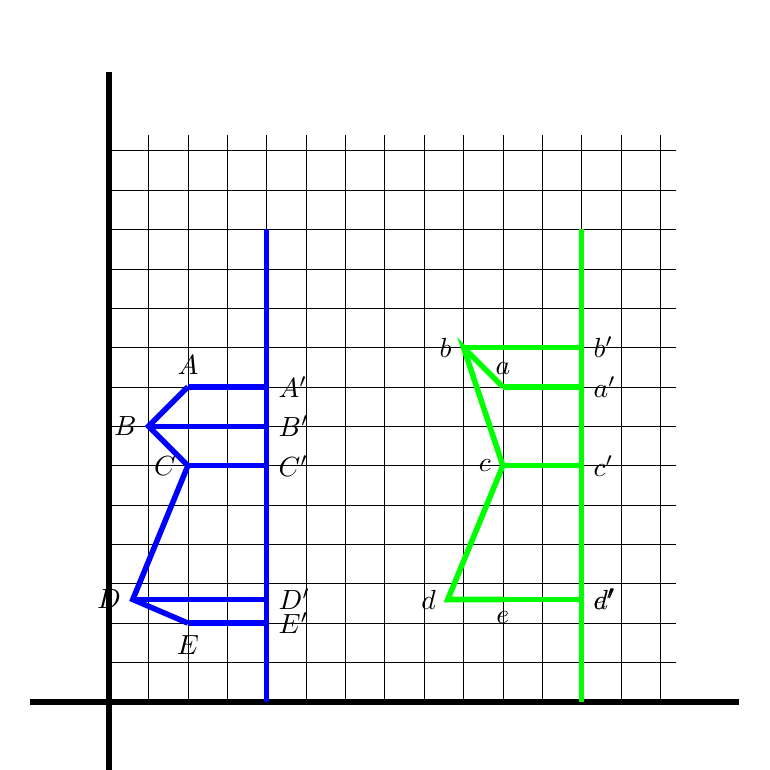
\begin{tikzpicture}[line width=2pt]
\draw (-1,0) -- (8,0);
\draw (0,-1) -- (0,8);
\draw[step=.5cm, very thin] (0,0) grid (7.2,7.2);

\coordinate [label=above:$A$] (A) at (1, 4);
\coordinate [label=left:$B$] (B) at (0.5, 3.5);
\coordinate [label=left:$C$] (C) at (1, 3);
\coordinate [label=left:$D$] (D) at (0.3, 1.3);
\coordinate [label=below:$E$] (E) at (1, 1);

\draw[blue] (A) -- (B) -- (C)  -- (D) -- (E);
\draw[blue] (2, 0) -- (2, 6);

\coordinate [label=right:$A'$] (A') at (2, 4);
\coordinate [label=right:$B'$] (B') at (2, 3.5);
\coordinate [label=right:$C'$] (C') at (2, 3);
\coordinate [label=right:$D'$] (D') at (2, 1.3);
\coordinate [label=right:$E'$] (E') at (2, 1);

\draw[blue] (A) -- (A');
\draw[blue] (B) -- (B');
\draw[blue] (C) -- (C');
\draw[blue] (D) -- (D');
\draw[blue] (E) -- (E');

\coordinate [label=above:$a$] (a) at (5, 4);
\coordinate [label=left:$b$] (b) at (4.5, 4.5);
\coordinate [label=left:$c$] (c) at (5, 3);
\coordinate [label=left:$d$] (d) at (4.3, 1.3);
\coordinate [label=below:$e$] (e) at (5, 1.3);

\draw[green] (a) -- (b) -- (c)  -- (d) -- (e);
\draw[green] (6, 0) -- (6, 6);

\coordinate [label=right:$a'$] (a') at (6, 4);
\coordinate [label=right:$b'$] (b') at (6, 4.5);
\coordinate [label=right:$c'$] (c') at (6, 3);
\coordinate [label=right:$d'$] (d') at (6, 1.3);
\coordinate [label=right:$e'$] (e') at (6, 1.3);

\draw[green] (a) -- (a');
\draw[green] (b) -- (b');
\draw[green] (c) -- (c');
\draw[green] (d) -- (d');
\draw[green] (e) -- (e');
\end{tikzpicture}
\caption{Monotonic polygonal chains}
\label{fig:monotonic_chain}
\end{figure}

\section{表格测试}
\begin{table}[htbp]
  \centering
  \begin{tabular}[htbp]{r|l}
    \toprule
    日期 & 任务 \\
    \midrule
    2011.5 & 完善此份文档 \\
    2011.6 & 完善安装脚本 \\
    \bottomrule
  \end{tabular}
  \caption{表格}
  \label{tab:table1}
\end{table}

\section{源代码高亮测试}

以下是\href{http://acm.zju.edu.cn/onlinejudge/showProblem.do?problemCode=1372}{ZOJ 1372}的解题c++代码:

\begin{lstlisting}[language=c++]
#include <iostream>
#include <string>
using namespace std;
 
const long max_points = 100;
const long infinity = 1000001;
 
int p, r, length, g[max_points][max_points];
bool flag;
 
class vertex
{
public:
    int distance;
    bool visited;
};
 
vertex v[max_points];
 
void initial()
{
    for(int i = 1; i <= p; i++)
        for(int j = 1; j <= p; j++)
            g[i][j] = infinity;
}
 
void prim(int origin)
{
    int temp_min;
    int temp_v = 0;
    int sum = 0;
 
    for(int i = 1; i <= p; i++)
    {
        v[i].distance = g[i][origin];
        v[i].visited = false;
    }
 
    v[origin].distance = 0;
    v[origin].visited = true;
 
    sum++;
 
    while (sum < p)
    {
        temp_min = infinity;
        for(int i = 1; i <= p; i++)
            if(v[i].visited == false && v[i].distance < temp_min)
            {
                temp_min = v[i].distance;
                temp_v = i;
            }
         
        if(temp_min < infinity)
        {
            length += v[temp_v].distance;
            v[temp_v].visited = true;
            sum++;
        }
        else
        {
            flag = true;
            break;
        }
 
        for(int i = 1; i <= p; i++)
        {
            if(v[i].visited == false && v[i].distance > g[i][temp_v])
            {
                v[i].distance = g[i][temp_v];
            }
        }
    }
}
 
int main(int argc, char *argv[])
{
    int a, b, c;
 
    while(cin >> p)
    {
        if(p == 0)
            break;
        cin >> r;
 
        initial();
 
        for(int i = 0; i < r; i++)
        {
            cin >> a >> b >> c;
            if(c < g[a][b])
                g[a][b] = g[b][a] = c;
        }
        length = 0;
        prim(1);
 
        cout << length << endl;
    }
 
    return 0;
} 
\end{lstlisting}

\section{数学公式测试}

著名的爱因斯坦质能方程(\ref{eq:emc2}):

\begin{equation}
  \label{eq:emc2}
  E=mc^2
\end{equation}

计算$f(x)=x^2$的不定积分(\ref{eq:2}):

\begin{equation}
  \label{eq:2}
  \int x^2 dx = \frac{1}{3} x^3
\end{equation}
\section{参考文件测试}
参考文件最好使用bibtex,关于bibtex的使用方法,你可以自行查阅相关文献。

这里是参考文献\cite{c_minigui}

%%%%%%%%%------------------------------------------------------------------------
%%%% 附录

% \appendix    
% \appendixpage
%% 将附录条目添加到contents
% \addappheadtotoc

%%%% 附录结束
%%%%%%%%------------------------------------------------------------------------

%
%%% 加入参考文献支持
%\bibliography{data/main}
%%% 解决目录中没有相应的参考文献的条目问题
%\addcontentsline{toc}{section}{\refname} 
%\end{document}
%%%% 正文部分结束
%%%%%%%%------------------------------------------------------------------------

%\restoregeometry
%\newpage

\tableofcontents
\setcounter{page}{-0}
\thispagestyle{empty}

\zihao{4}

\jxhj{%教学后记
	 }
\skrq{%授课日期
	2017年9月~ 日  }
\ktmq{%课题名称
	数控编程概术 }
\jxmb{%教学目标,每行前面要加 \item
	\item 巩固上期的基本指令;

	\item 总结上期的编程思路;

	\item 总结机床的操作技巧;

	\item 了解本期的学习内容及学生情况;}
\jxzd{%教学重点,每行前面要加 \item
	\item 巩固上期的基本指令;
	\item 总结上期的编程思路;}
\jxnd{%教学难点,每行前面要加 \item
	\item 总结上期的编程思路;}
\jjff{%教学方法
	通过讲述、举例、演示法来说明;}

\makeshouye %制作教案首页

%%%%教学内容
\subsection{组织教学}
\begin{enumerate}[\hspace{2em}1、]
	\setlength{\itemsep}{0pt}
	\item 集中学生注意力;
	\item 清查学生人数;
	\item 维持课堂纪律;
\end{enumerate}
\subsection{复习导入及主要内容}
\begin{enumerate}[\hspace{2em}1、]
\item 自我介绍
\item 企业需要什么样的数控人才:\\
A:人品好:有道德、有理想、乐于助人。\\
B:精神面貌好:胆大心细,勇于思考、
能吃苦,不怕累、不怕脏。\\
C:能干事,有水平、速度快。\\
D:积极上进,乐于创新
\item 学习目标及要求:\\
A:会操作数控机床。快,准、细心。\\
B:能进行简单零件的工艺处理。会、经验积累。 \\
C:能进行简单零件的编程。思路清晰、编程细心、改错准快。\\
\end{enumerate}
跟着老师、多练习(作业)、准备充分、多想多问多看。
\subsection{教学内容及过程}
\subsubsection{基本概念} \marginpar{说明介绍}
\paragraph{数控技术}
\paragraph{数控机床}
\paragraph{实习教学计划}

\subsubsection{手工编程复习} \marginpar{互动提问}
%如下面的思维导图 \ref{手工编程思维导图}
%\begin{figure}[!hbtp]	
%	\includegraphics{images/tu1} 
%	\caption{手工编程思维导图}\label{手工编程思维导图}
%\end{figure}

%\subsubsection{数控机床的操作}
%如下面的思维导图 \ref{数控机床的操作思维导}
%\begin{figure}[!hbtp]	
%	\includegraphics{images/tu2} 
%	\caption{数控机床的操作思维导图} \label{数控机床的操作思维导}
%\end{figure}

\subsubsection{数控机床指令}
\paragraph{G指令}\begin{itemize}
	\item G0 G1 G2 G3

	\item G17 G18 G19

	\item G9 G61 G62 G63 G64

	\item G4 \marginpar{说明介绍说明介绍说明介绍说明介绍说明介绍说明介绍}

	\item G20 G21

	\item G40 G41 G42 

	\item G43 G44 G49 \marginpar{说明介绍说明介绍说明介绍说明介绍说明介绍说明介绍}

	\item G90 G91

	\item G98 G99

	\item G81 G82 G83 G84 G85 G86 G87 G88 G89 G80 G73 G74 G76

\end{itemize}

\paragraph{M指令}

\begin{itemize}
	\item M0 M1 M2 M30

	\item M3 M4 M5 M19 

	\item M6 M7 M8 M9

	\item M98 M99

\end{itemize}

\paragraph{其它指令}
\subsubsection{常见加工结构}
\begin{itemize}
	\item 平面

	\item 外轮廓

	\item (岛屿)

	\item 孔
	\item 凸轮槽

	\item 复杂零件

	\item 配合零件

	\item CAD/CAM

	\item 宏程序

	\item 其它
\end{itemize}
\subsubsection{上学期期末试卷分析}
\subsection{课堂小结}
主要复习了数控方面的基本知识。
\vfill
\subsection{布置作业}
\begin{enumerate}[1、]
	\item 自选一零件图, 写出其工艺与程序;

	\item 写出如图所示零件的程序及与工艺;
\end{enumerate}
\vfill

\jxhj{%教学后记
	}
\skrq{%授课日期
	}
\ktmq{%课题名称
	学习新内容 }
\jxmb{%教学目标,每行前面要加 \item
	\item 巩固上期的基本指令;

	\item 总结上期的编程思路;

	\item 总结机床的操作技巧;

	\item 了解本期的学习内容及学生情况;}
\jxzd{%教学重点,每行前面要加 \item
	\item 巩固上期的基本指令;

	\item 总结上期的编程思路;}
\jxnd{%教学难点,每行前面要加 \item
	\item 总结上期的编程思路;}
\jjff{%教学方法
	通过讲述、举例、演示法来说明;}

\makeshouye %制作教案首页

%%%%教学内容
\subsection{组织教学}
\begin{enumerate}[\hspace{2em}1、]
	\item 集中学生注意力;
	\item 清查学生人数;
	\item 维持课堂纪律;
\end{enumerate}
\subsection{复习导入及主要内容}
\begin{enumerate}[\hspace{2em}1、]
	\item 上学期末考试讲评;

	\item 了解学生情况;
\end{enumerate}
\subsection{教学内容及过程}
\subsubsection{本期教学安排} \marginpar{说明介绍}
\paragraph{理论教学计划:}
\begin{itemize}
	\item 复习上期内容

	\item 两面加工实例

	\item 变量与基本运算

	\item 椭圆加工if  goto

	\item 循环及其指令 if goto while

	\item 循环应用

	\item Siemens参数编程概述

	\item Siemens应用

	\item 镜象指令的使用

	\item 薄壁及配合件加工工艺

	\item 双曲线、抛物线加工

	\item 孔系加工(循环嵌套)

	\item 圆孔的宏程序

	\item 方槽椭圆槽的宏程序
	\item 斜面与圆柱面的宏程序

	\item 球面的宏程序(凸/凹)

	\item 椭球面的宏程序

	\item 任意轮廓倒圆角(系统变量)

	\item 任意轮廓倒圆角(G10)

	\item Siemens上倒角与倒圆

	\item 宏程序调用基本知识

	\item 宏程序调用的应用

	\item 多轴加工概述

	\item 四轴加工:圆柱凸轮的加工

	\item 五轴加工简介

	\item 综合练习(一)

	\item 综合练习(二)

	\item 综合练习(三)

	\item 综合练习(四)

\end{itemize}

\subparagraph{实习教学计划}
\begin{itemize}
	\item 两面加工类零件加工

	\item 薄壁配合件加工

	\item 宏程序加工

	\item 综合加工(钢材)
\end{itemize}

\subsubsection{手工编程复习} \marginpar{互动提问}
如下面的思维导图 \ref{手工编程思维导图}
\begin{figure}	
	\includegraphics{images/图片1} 
	\caption{手工编程思维导图}\label{手工编程思维导图}
\end{figure}

\subsubsection{数控机床的操作}
如下面的思维导图 \ref{数控机床的操作思维导}
\begin{figure}	
	\includegraphics{images/图片2} 
	\caption{数控机床的操作思维导图} \label{数控机床的操作思维导}
\end{figure}

\subsubsection{数控机床指令}
\paragraph{G指令}\begin{itemize}
	\item G0 G1 G2 G3

	\item G17 G18 G19

	\item G9 G61 G62 G63 G64

	\item G4 

	\item G20 G21

	\item G40 G41 G42 

	\item G43 G44 G49

	\item G90 G91

	\item G98 G99

	\item G81 G82 G83 G84 G85 G86 G87 G88 G89 G80 G73 G74 G76

\end{itemize}

\paragraph{M指令}

\begin{itemize}
	\item M0 M1 M2 M30

	\item M3 M4 M5 M19

	\item M6 M7 M8 M9

	\item M98 M99

\end{itemize}

\paragraph{其它指令}
\subsubsection{常见加工结构}
\begin{itemize}
	\item 平面

	\item 外轮廓

	\item (岛屿)

	\item 孔
	\item 凸轮槽

	\item 复杂零件

	\item 配合零件

	\item CAD/CAM

	\item 宏程序

	\item 其它
\end{itemize}
\subsubsection{上学期期末试卷分析}
\subsection{课堂小结}
主要复习了数控方面的基本知识。
\vfill
\subsection{布置作业}
\begin{enumerate}[1、]
	\item 自选一零件图, 写出其工艺与程序.

	\item 写出如图所示零件的程序及与工艺.
\end{enumerate}
\jxhj{%教学后记
	}
\skrq{%授课日期
	2017年3月6日 4-5节}
\ktmq{%课题名称
	变量Z向分层}
\jxmb{%教学目标,每行前面要加 \item
	\item 掌握用循环来实现Z向分层;
	\item 掌握条件表达式的确定(加不加“=”);
	\item 掌握if then的使用;}
\jxzd{%教学重点,每行前面要加 \item
	\item 循环来实现Z向分层;
	\item 条件表达式的确定(加不加“=”)}
\jxnd{%教学难点,每行前面要加 \item
	\item 条件表达式的确定(加不加“=”)}
\jjff{%教学方法
	通过讲述、举例、演示法来说明;}

\makeshouye %制作教案首页

%%%%教学内容
\subsection{组织教学}
\begin{enumerate}[\hspace{2em}1、]
	\item 集中学生注意力;
	\item 清查学生人数;
	\item 维持课堂纪律;
\end{enumerate}
\subsection{复习导入及主要内容}
\begin{enumerate}[\hspace{2em}1、]
\item 变量与常量;
\item Fanuc上的变量;
\item 变量的分类;
\item 运算;
\item 运算顺序与括号
\end{enumerate}
\subsection{教学内容及过程}
\subsubsection{Z向分层} \marginpar{举例说明}
\paragraph{基本思路} 
以前 G91+子程序。

G90 深度用 变量,每个深度进行计算。

G91 次数用 变量,次数递增记数。

\paragraph{形成循环:}
\begin{verbatim}
#1=0
N10 
#1=#1+4
G90 G1 z-#1
……
If [#1lt12] goto10

#1=0
N10
#1=#1+1
G91 g1 z-4.0
……
If [#1lt3] goto10
\end{verbatim}
尽量用G90。

\paragraph{思考一}
如果初始值为4,侧程序怎么改

\begin{verbatim}
#1=4
N10 
G90 G1 z-#1
……
#1=#1+4
If [#1    12] goto10
\end{verbatim}

讨论分析:

用  LE 
 
结论:

\#1=\#1+4 放在执行之前,判断的量是当前位置值,当前值为终点是,应结束循环,条件判断用 GT 或 LT

\#4=\#4+4 放在执行之后,判断的量是下一个位置的值,下一点为终止值时,应走到终点后结束循环,条件判断应用GE或LE。


\paragraph{思考二}

当加工深度为13mm时怎么改程序。

方法一:等分每层加工 13/4=3.25mm

方法二:第一层加工1mm 其余12/4=3mm

\#1=2    \#1=\#1-3

注意初始值的更换。

方法三:每层4mm 最后一层1mm

怎么实现?

\#1=0  \#1=\#1-4  到了16?

\subsubsection{IF  Then 指令}

格式:  if [条件] THEN [指令]

功能: 条件成立时 执行 THEN 后的指令

条件不成立时,跳过后面的指令。

如 if [\#1GT13] THEN \#1=13

不适合判断的是下一个值,会干涉判断。


\subsubsection{Z向分层的应用}
\begin{verbatim}
#1=0
N10 
#1=#1+4
If [#1 GT 13] then #1=13
G90 G1 z-#1
……
If [#1lt13] goto10
写成while就是:
#1=0
While [#1 lt 13] DO1
#1=#1+4
If [#1 GT 13] then #1=13
G90 G1 z-#1
……
END1
\end{verbatim}

实例:深度13

\subsection{课堂小结}

\begin{enumerate}[1、]
	\item Z向分层
	\item IF Then
	\item 应用
\end{enumerate}

\vfill
\subsection{布置作业}
\begin{enumerate}[1、]
	\item 自选1个图进行Z向分层应用。 
\end{enumerate}
\vfill
\jxhj{%教学后记
	}
\skrq{%授课日期
	2017年3月13日 4-5节}
\ktmq{%课题名称
	椭圆编程 }
\jxmb{%教学目标,每行前面要加 \item
	\item 掌握用循环来实现Z向分层;
	\item 掌握椭圆的宏程序思路;
	\item 掌握椭圆的宏程序。 }
\jxzd{%教学重点,每行前面要加 \item
	\item 循环来实现Z向分层;
	\item 椭圆的宏程序思路。 }
\jxnd{%教学难点,每行前面要加 \item
	\item 椭圆的宏程序思路。 }
\jjff{%教学方法
	通过讲述、举例、演示法来说明;}

\makeshouye %制作教案首页

%%%%教学内容
\subsection{组织教学}
\begin{enumerate}[\hspace{2em}1、]
	\item 集中学生注意力;
	\item 清查学生人数;
	\item 维持课堂纪律;
\end{enumerate}
\subsection{复习导入及主要内容}
\begin{enumerate}[\hspace{2em}1、]
\item Z向分层;
\item IF THEN 指令;
\item Z向分层的应用;
\end{enumerate}
\subsection{教学内容及过程}
\subsubsection{非圆曲线的拟合加工} %\marginpar{举例说明}
 数控机床一般中能作直线插补和圆弧插补. 遇到工件轮廓是非圆曲线的零件时. 常用直线段或圆弧去逼近非圆曲线. 即拟合加工. 只要拟合误差在允许的范围内就行了.
 
 \paragraph{分段}
 等插补段法(求最小曲率半径Rmin, 求在允许插补误差时的弦长,求坐标)
 
 等插补误差法(以起点建立误差圆, 求该圆与曲线的公切线的斜率, 以起点作公切线的平行线, 计算坐标.)
 
 其它方法: (等角度)
 
\paragraph{用直线拟合}
 弦线, 割线, 切线
 \paragraph{圆弧逼近法}
 通过三点作圆(这三点是上面分段中的三个点)
 
 计算圆心
 
 计算坐标
 
\subsubsection{椭圆的数学模型}
\paragraph {参数方程}
 $$X=A*cos(a)$$
 $$Y=B*sin(a)$$
  使用角度控制
\paragraph{ 普通方程}
 $$ \frac{X^2}{A^2} + \frac{Y^2}{B^2} =1 $$
  可使用$X$控制, 常用于车床
\subsubsection{流程控制}
\subsubsection{椭圆的宏程序}
\begin{verbatim}
N100 #3=#3-1
G1 X[#1*COS[#3]] Y[#1*SIN[#3]]
IF [#1 GT -180] GOTO100
\end{verbatim}
\subsubsection{GOTO指令}
无条件转移。
 
\subsection{课堂小结}

\begin{enumerate}[1、]
	\item 非圆曲线的拟合加工;
	\item 椭圆的数学模型;
	\item 流程控制
	\item 椭圆的宏程序
\end{enumerate}

\vfill
\subsection{布置作业}
\begin{enumerate}[1、]
	\item 编写一个比较通用的外圆加工轮廓。。 
\end{enumerate}
\vfill
\jxhj{%教学后记
	}
\skrq{%授课日期
	2017年9月21日 4-5节}
\ktmq{%课题名称
	基本指令(二) }
\jxmb{%教学目标,每行前面要加 \item
	\item 掌握G2/G3半径-R的使用;
    \item 掌握G2/G3圆心编程的使用;
    \item 能用G2/G3进行程序的编写;
    \item 掌握编写数控程序的基本思路。}
\jxzd{%教学重点,每行前面要加 \item
	\item G2/G3半径-R的使用;
	\item G2/G3圆心编程的使用;}
\jxnd{%教学难点,每行前面要加 \item
	\item G2/G3圆心编程的使用;}
\jjff{%教学方法
	通过讲述、举例、演示法来说明;}

\makeshouye %制作教案首页

%%%%教学内容
\subsection{组织教学}
\begin{enumerate}[1、]
	\item 集中学生注意力;
	\item 清查学生人数;
	\item 维持课堂纪律;
\end{enumerate}
\subsection{复习导入及主要内容}
\begin{enumerate}[1、]
\item 案例分析;
\item 指令讲解G2/G3;
\item 编写程序;
\item 编写程序的基本思路。
\end{enumerate}

\textbf{案例分析}

在数控铣床或加工中心上加工如图\ref{fig:4-1}所示的零件,试完成程序的编写,已知毛坯为 $\Phi$ 110*30。

\begin{figure}[h]
    \centering
    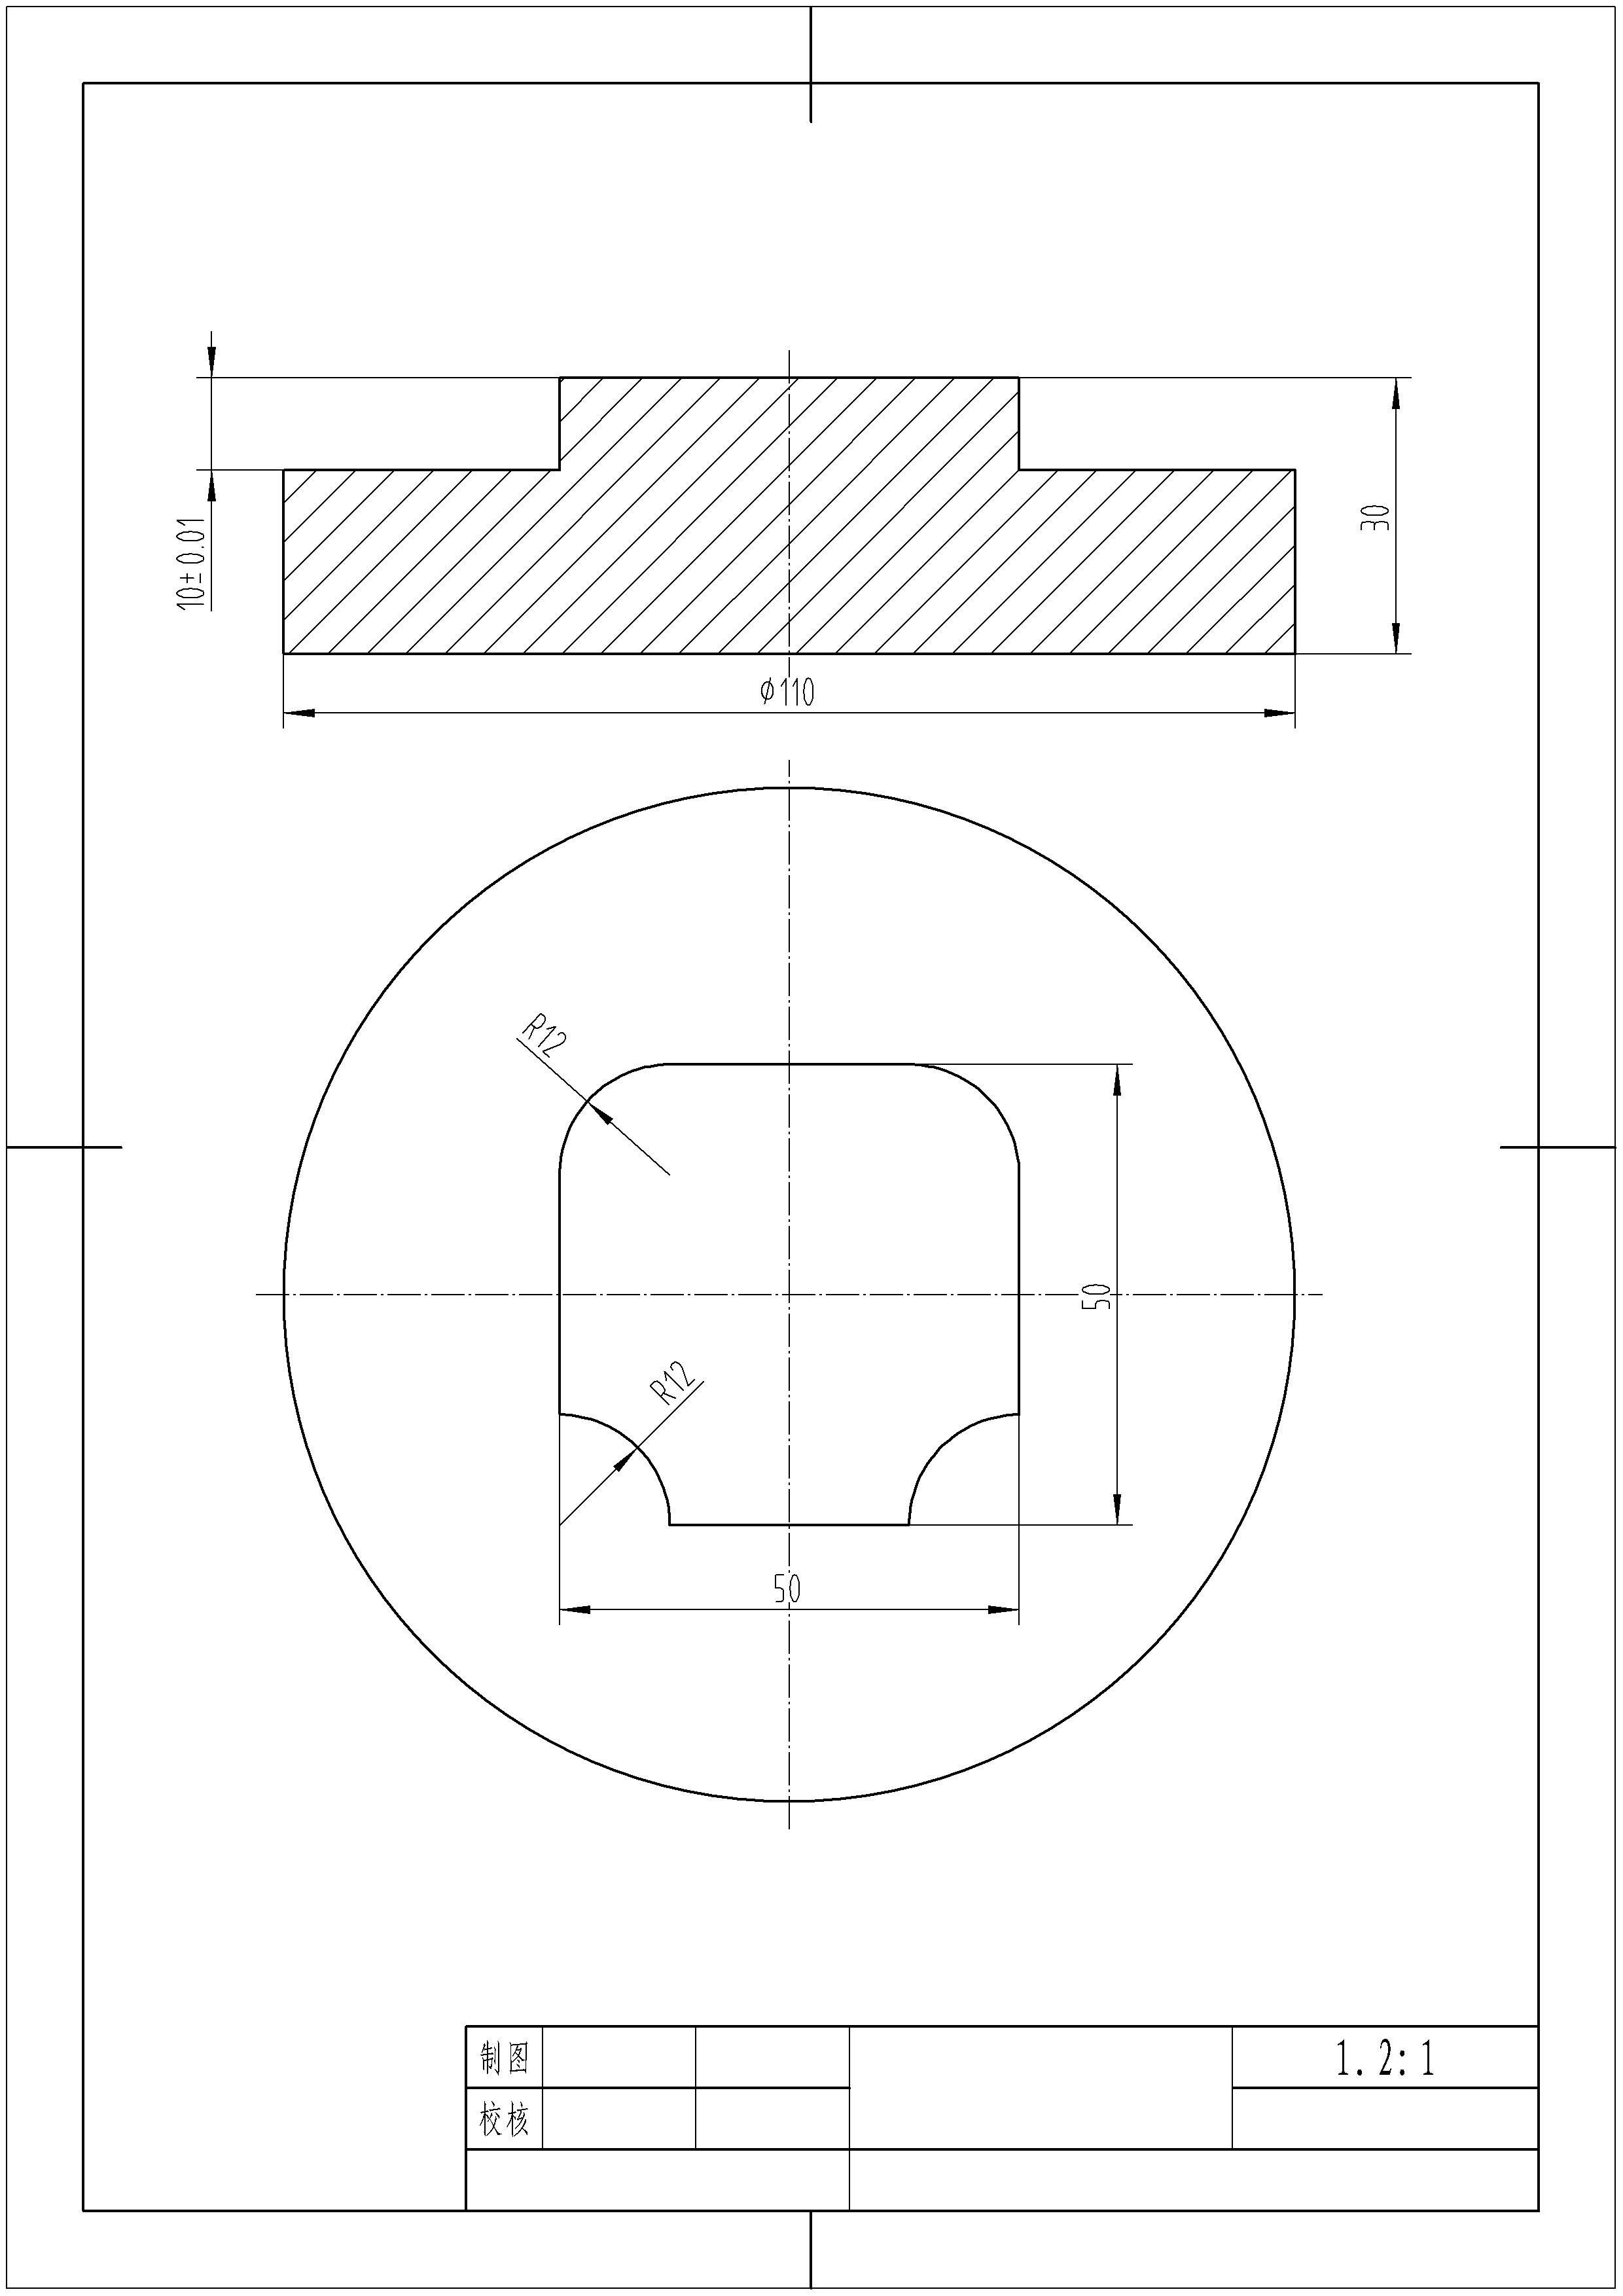
\includegraphics[width=0.8\linewidth,trim=50 150 50 100,clip]{data/image/5-1.jpg}
    \caption{}
    \label{fig:4-1}
\end{figure}

\begin{enumerate}[1、]
    \item 图样分析;
    \item 确定加工内容;
    \item 确定装夹及工件坐标系;
    \item 确定刀具及切削用量;
    \item 确定工序及走刀路线;
    \item 计算点坐标;
    \item 编写程序单。
\end{enumerate}

\subsection{教学内容及过程}

\subsubsection{案例分析}

在数控铣床或加工中心上加工如图\ref{fig:4-1}所示的零件,试完成程序的编写,已知毛坯为 $\Phi$ 110*30。

\begin{figure}[h]
    \centering
    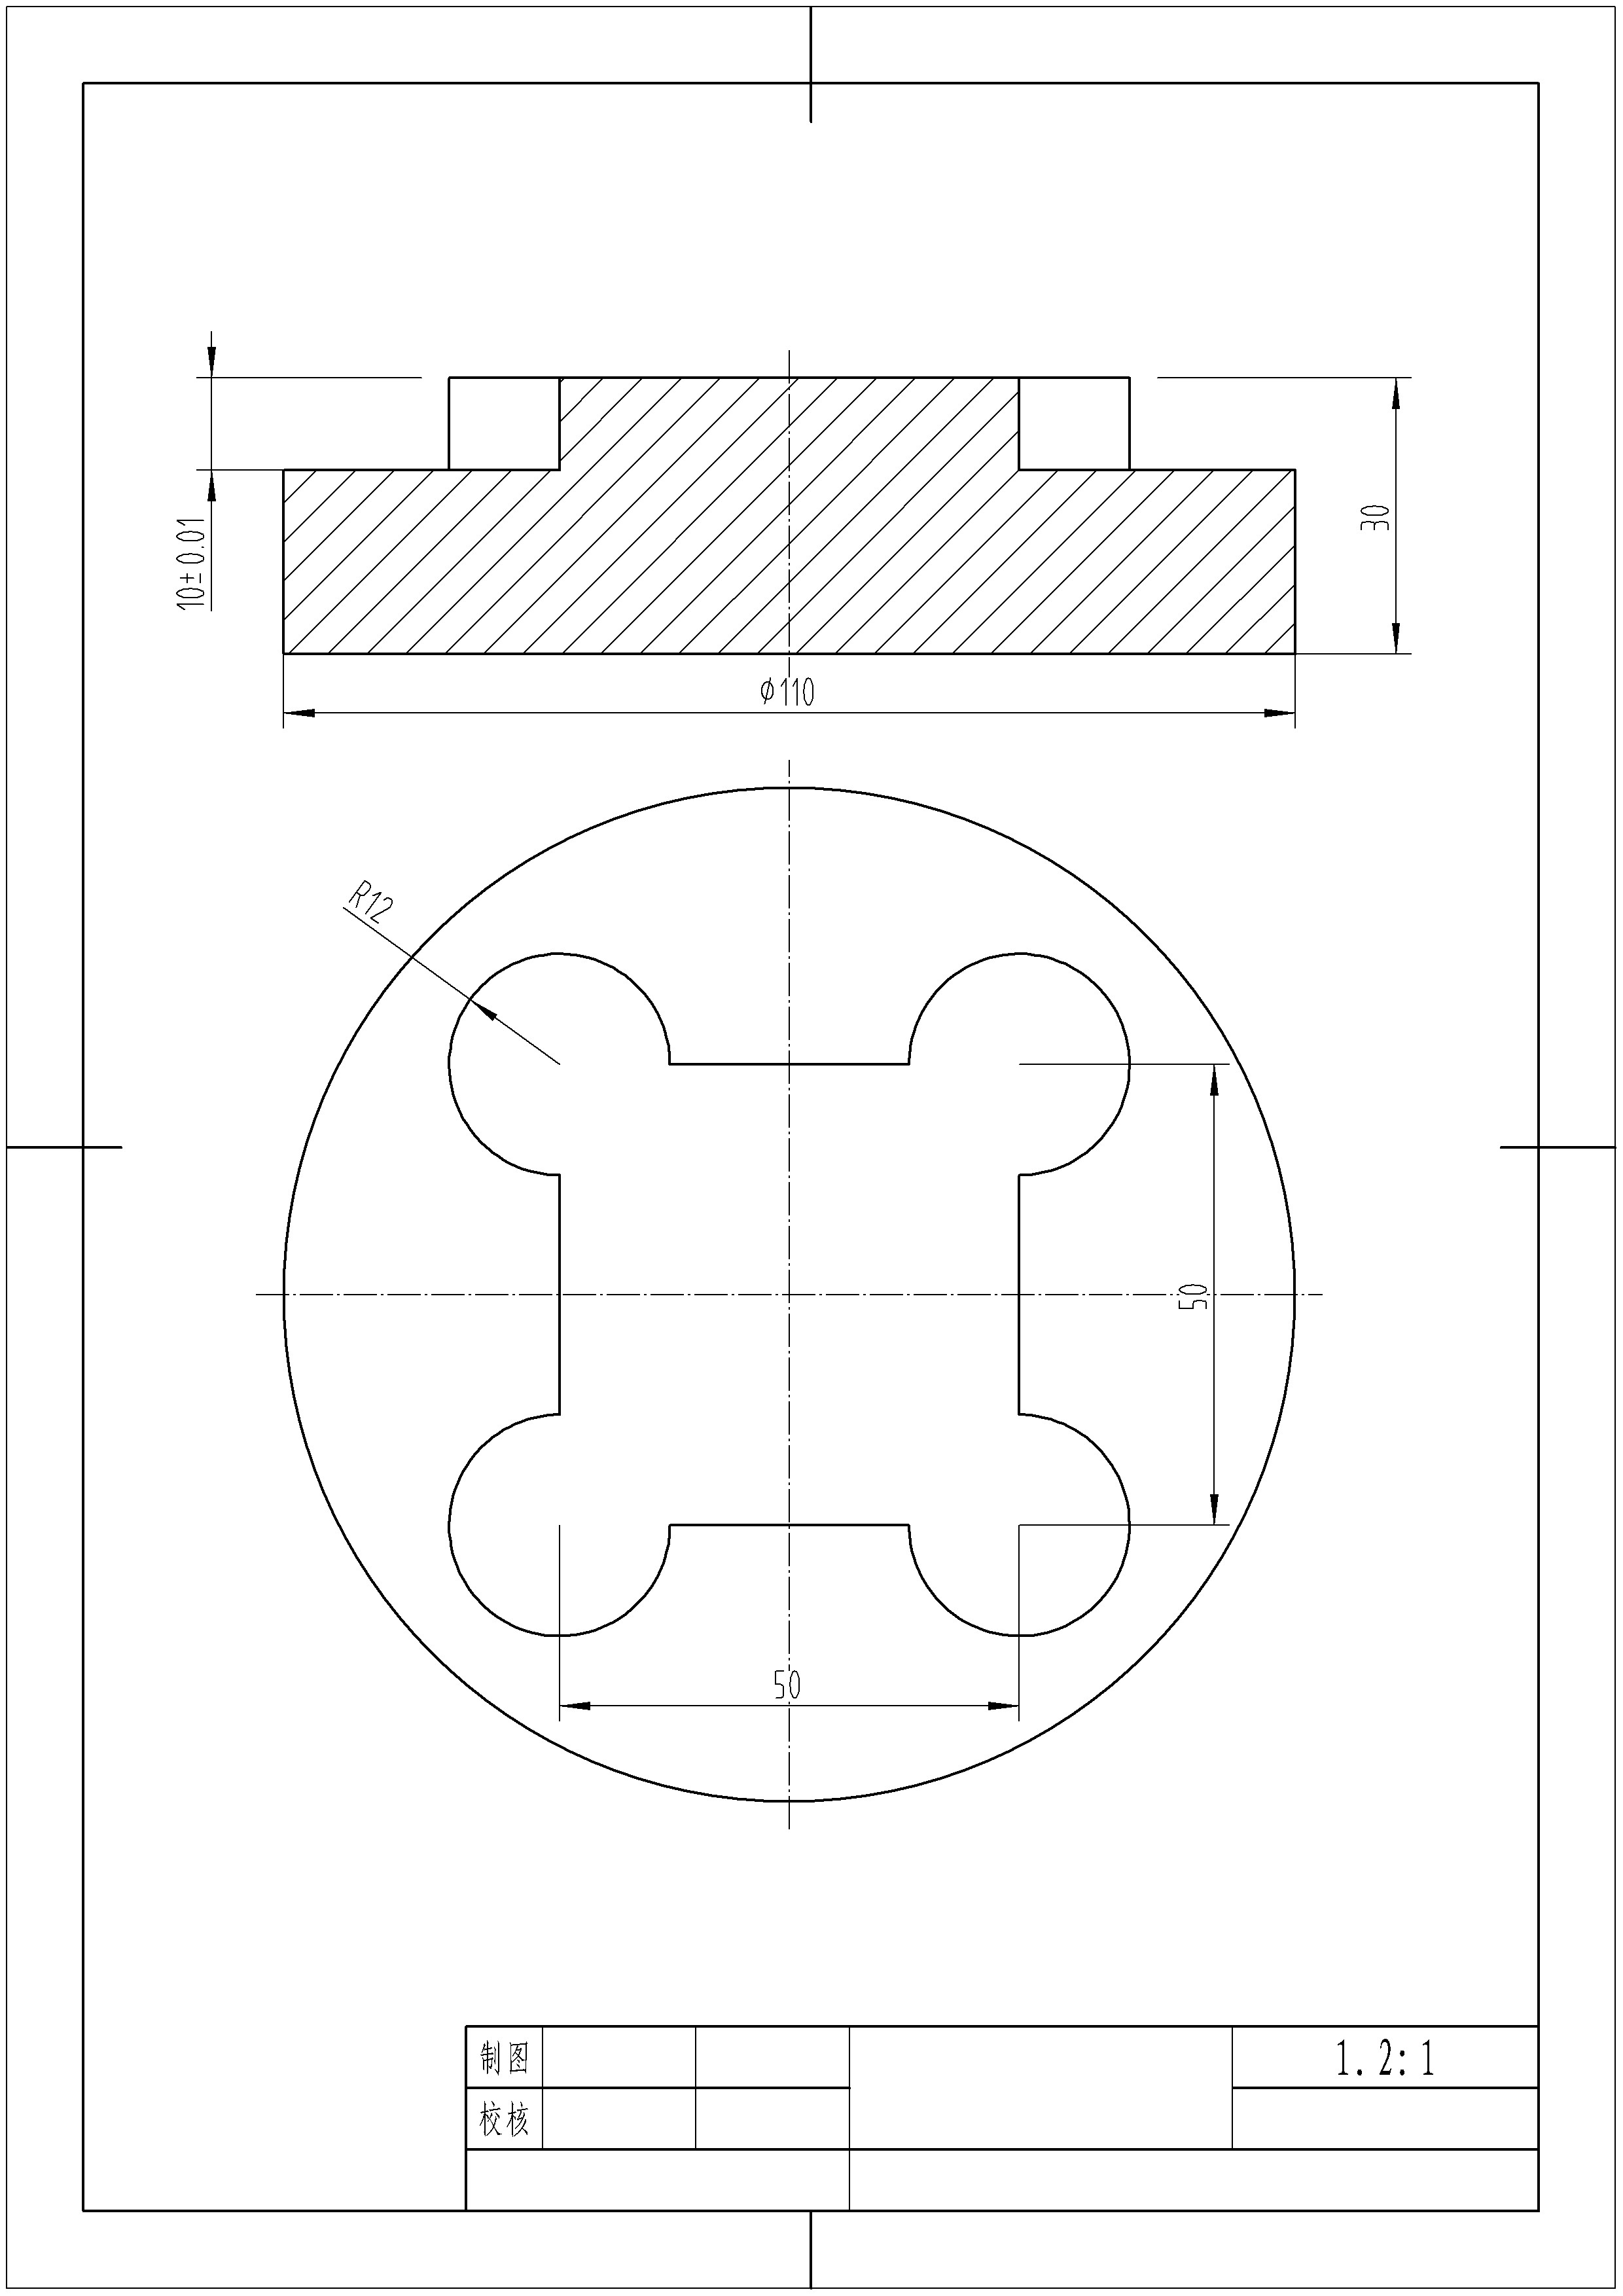
\includegraphics[width=0.8\linewidth,trim=50 150 50 100,clip]{data/image/5-2.jpg}
    \caption{}
    \label{fig:4-1}
\end{figure}

\begin{enumerate}[1、]
    \item 图样分析;
    \item 确定加工内容;
    \item 确定装夹及工件坐标系;
    \item 确定刀具及切削用量;
    \item 确定工序及走刀路线;
    \item 计算点坐标;
    \item 编写程序单。
\end{enumerate}


路径特点:

圆弧的圆心角大于180度,显然不能直接用前面的程序。

解决方法:解决方法:



1、把圆弧分成多个圆心角小于180度的圆弧。

2、掌握圆心角大于180度圆弧指令的使用。

当圆心角大于180度时,用负的半径值来表示。

当圆心角小于180度时,用正的半径值来表示。

Siemens上用CR= 正负规则一样。



\subsubsection{整圆编程}
在数控铣床或加工中心上用整圆的路径进行面铣,面铣深度为1mm,试完成加工成型的编写。
\begin{figure}[h]
    \centering
    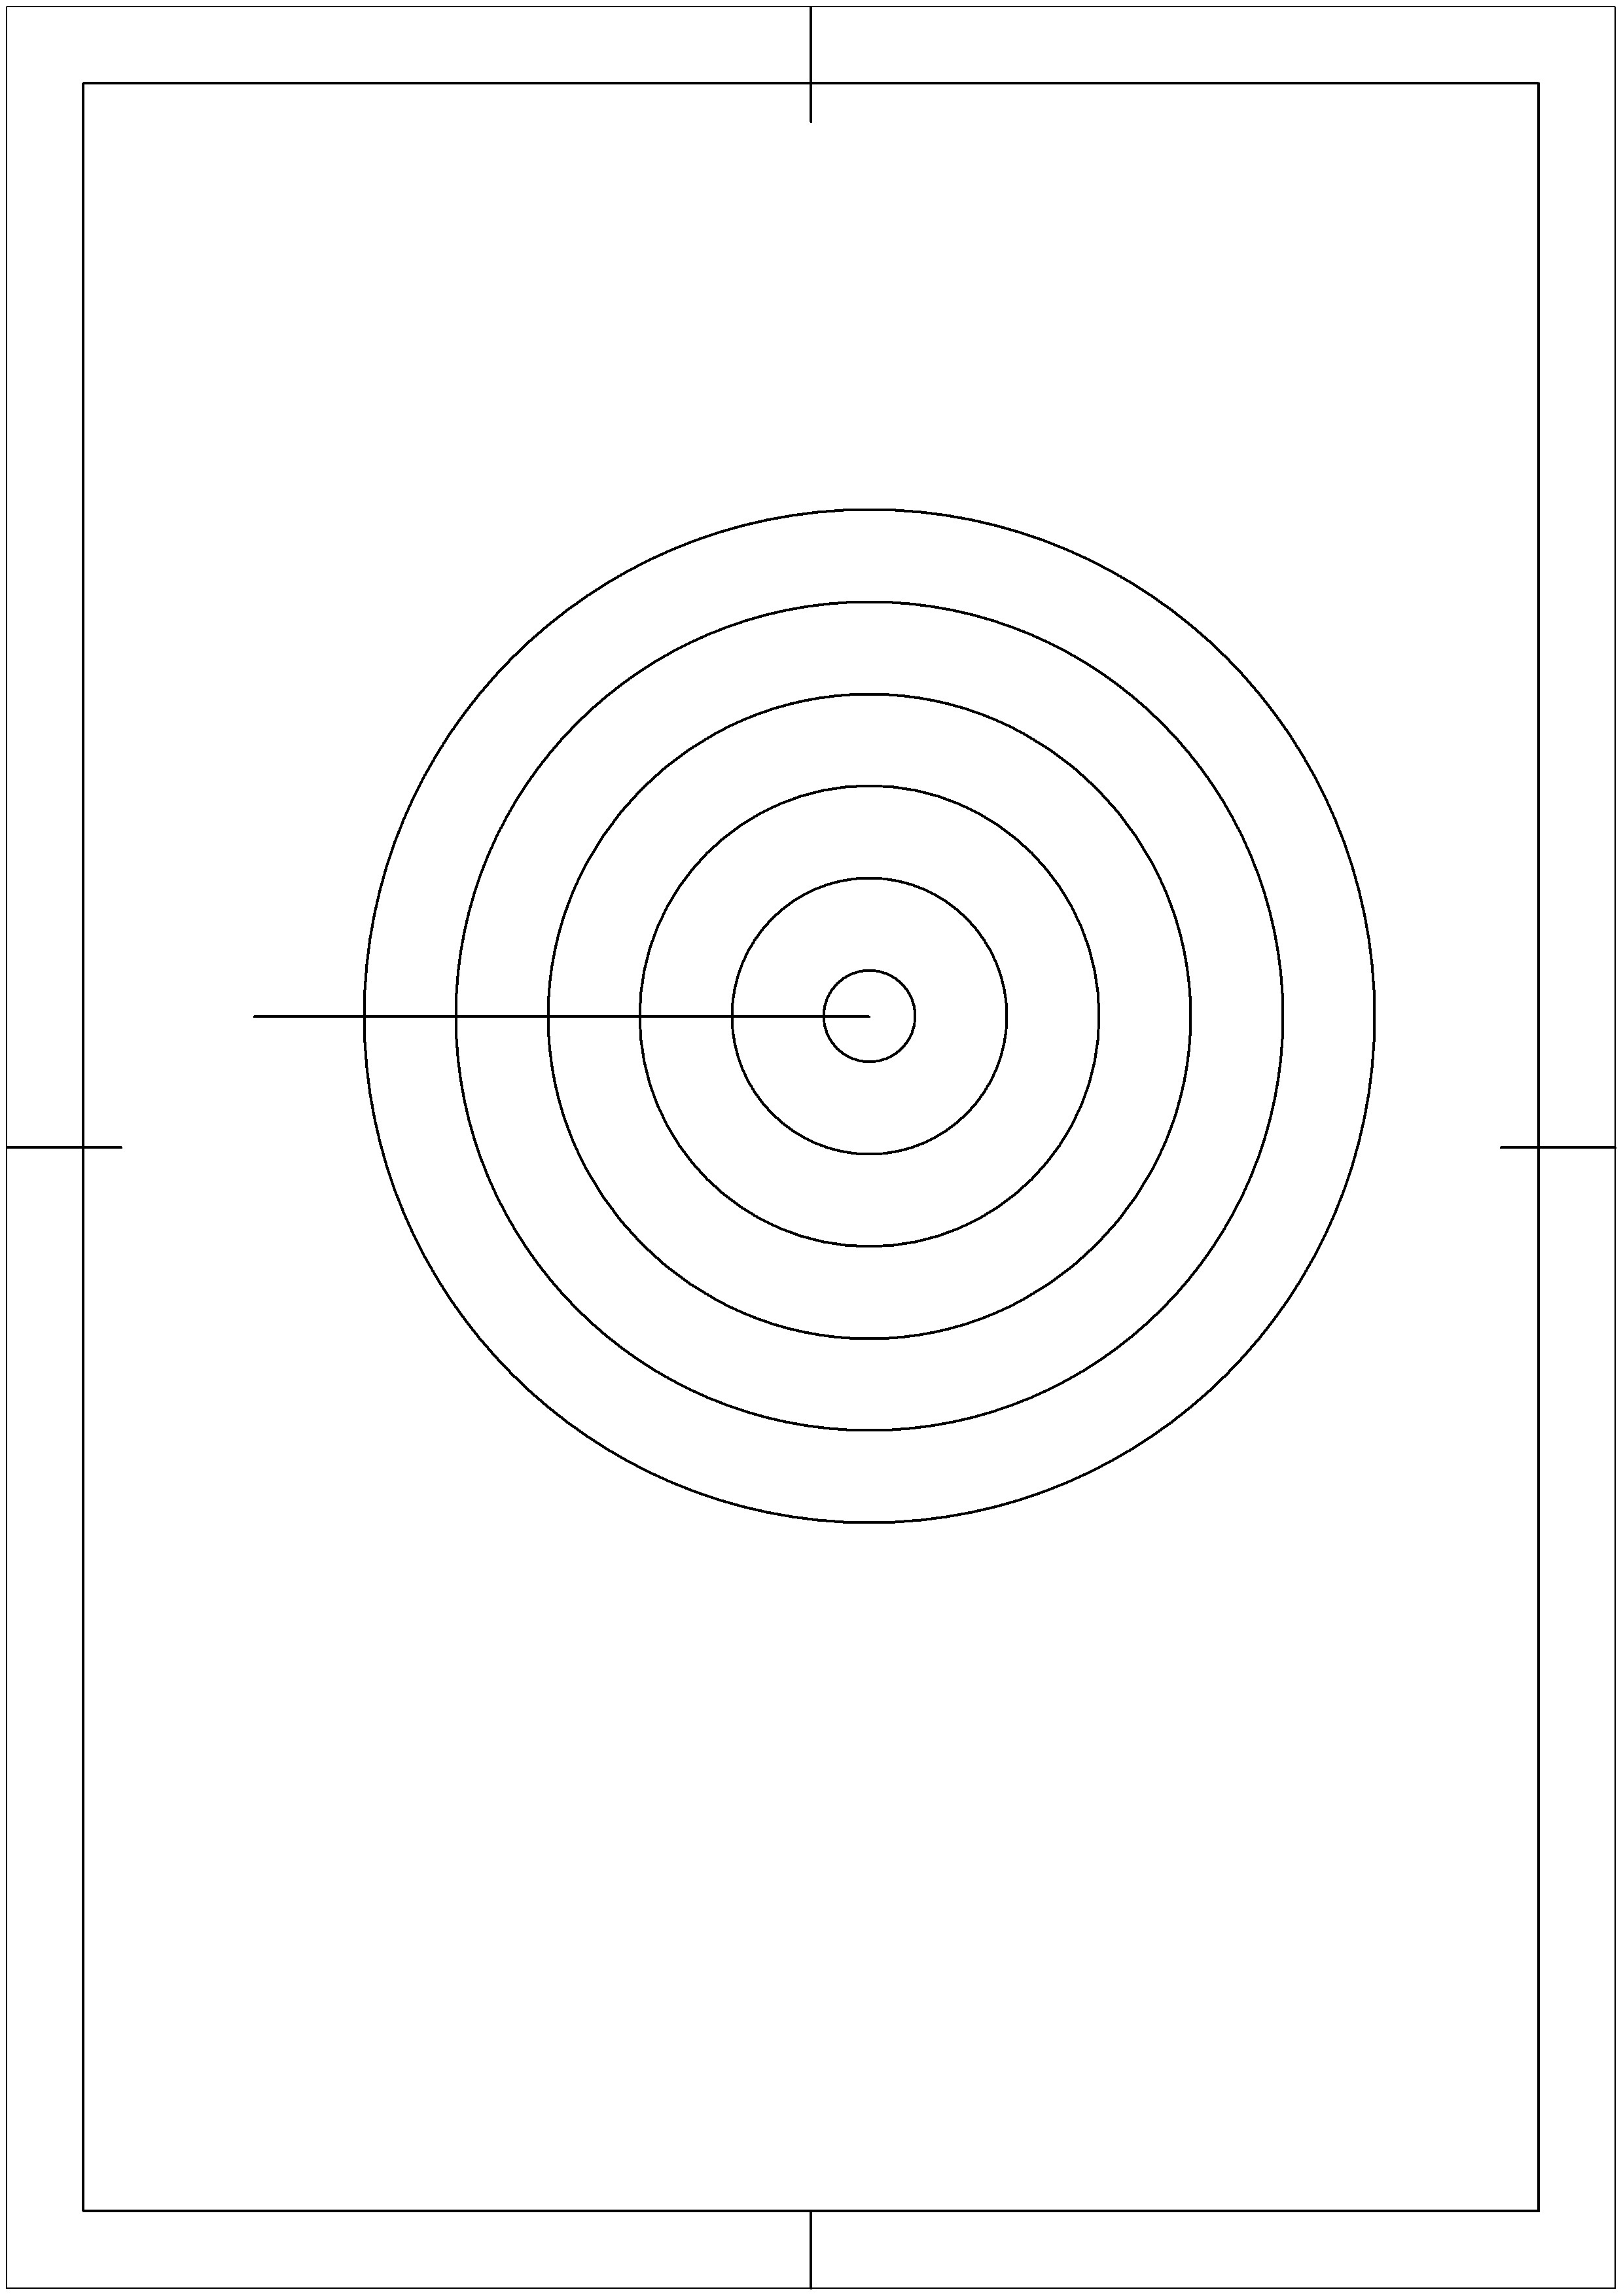
\includegraphics[width=0.8\linewidth,trim=50 150 50 100,clip]{data/image/5-3.jpg}
    \caption{}
    \label{fig:5-3}
\end{figure}

整圆路径也可以分成多个圆弧。

一个整圆路径可以用IJK圆心来编程。

不能用半径来编写一个整圆。


I、J、K表示圆心相对于起点的坐标。即:

I=X圆心-X起点

J=Y圆心-Y起点

K=Z圆心-Z起点

I、J、K与G90/G91无关,只与整圆的起点有关。

如: G17 G90 G2 X-50.0 Y-50.0 I50.0 J0;

参考程序:

\begin{lstlisting}
O0001;
G54G17G90;
M3S500;
G1Z30.0F2000;
X-65.Y0;
Z5.0;
Z-1.0F200;
X-55.0;
G2X-55.0Y0I55.0;
G1X-45.0;
G2I45.0;
G1X-35.0;
G2I-35.0;
G1X-25.0;
G2I-25.0;
G1X-15.0;
G2I-15.0;
G1X-5.0;
G2I5.0;
G1Z5.0;
Z30.0F2000;
M5;
M30;
\end{lstlisting}

\subsubsection{I、J、K的应用}
在数控铣床或加工中心上加工如图所示的零件,试用I、J、K完成程序的编写。
\begin{figure}[h]
    \centering
    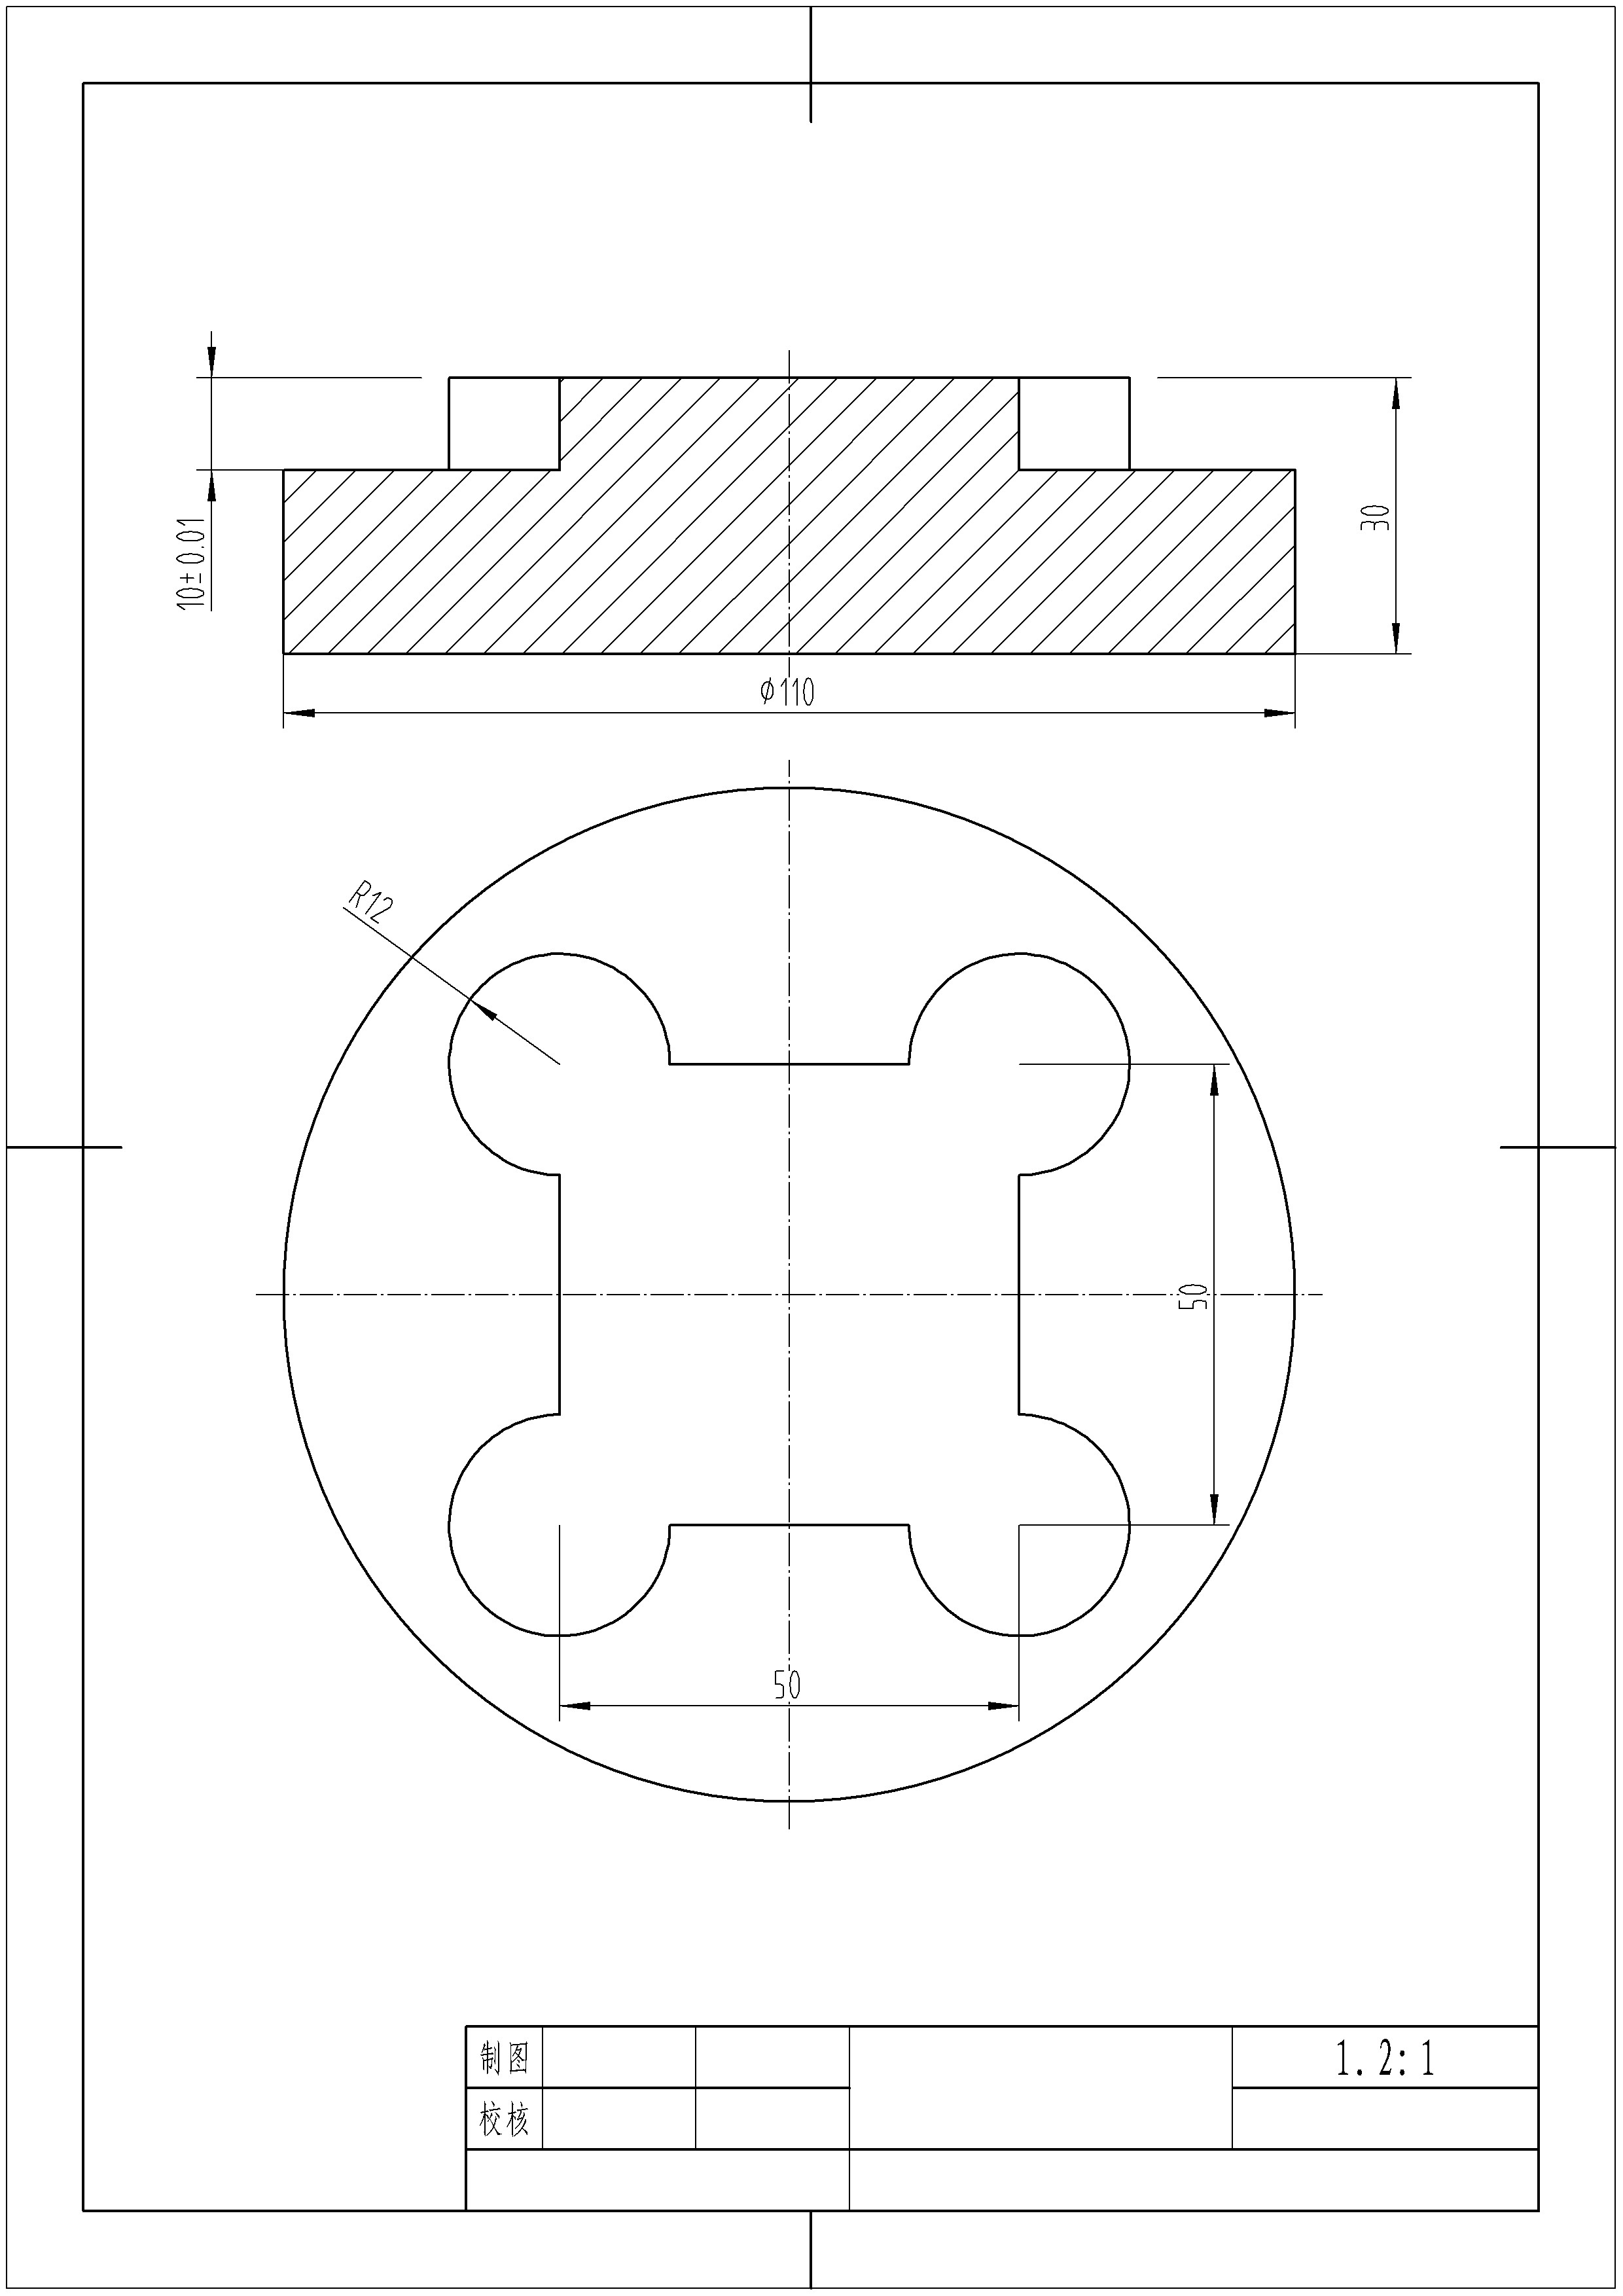
\includegraphics[width=0.8\linewidth,trim=50 150 50 100,clip]{data/image/5-4.jpg}
    \caption{}
    \label{fig:5-4}
\end{figure}
参考程序:

\begin{lstlisting}
O0001;
G54G17G90;
M3S500;
G1Z30.0F2000;
X-65.0Y0;
Z5.0;
Z-10.0F2000;
X-25.0;
Y13.0;
G2X-13.0Y25.0J13.0;
G1X13.0;
G2X25.0Y13.OJ-13.0;
….
\end{lstlisting}






手工编程中,能用半径编程就用半径编程,一般零件图标的是半径,也不容易出错。

自动编程,可以输出I、J、K以增加程序在不同机床通用性。


\subsubsection{编写程序的基本思路}
程序初始化(安全保护)--------辅助准备(换刀,主轴启动,切削液开)--------定位到起刀点--------快速下刀--------工进下刀--------走加工轮廓--------提刀---------快速提刀到安全平面-------程序结束(换刀,主轴停止,切削液关,程序返回等)
\subsection{课堂小结}
\begin{enumerate}[1、]
\item 案例分析;
\item 指令讲解;
\item 编写程序;
\item 编写程序的基本思路。
\end{enumerate}
\vfill
\subsection{布置作业}
\begin{enumerate}[1、]
	\item 自定尺寸,编写加工一个矩形外形的程序?
\end{enumerate}
\vfill
\jxhj{%教学后记
}
\skrq{%授课日期
	2017年9月26日 4-5节}
\ktmq{%课题名称
	基本指令(三) }
\jxmb{%教学目标,每行前面要加 \item
	\item 掌握G2/G3半径-R的使用;
	\item 掌握G2/G3圆心编程的使用;
	\item 能用G2/G3进行程序的编写;
	\item 掌握编写数控程序的基本思路。}
\jxzd{%教学重点,每行前面要加 \item
	\item G2/G3半径-R的使用;
	\item G2/G3圆心编程的使用;}
\jxnd{%教学难点,每行前面要加 \item
	\item G2/G3圆心编程的使用;}
\jjff{%教学方法
	通过讲述、举例、演示法来说明;}

\makeshouye %制作教案首页

%%%%教学内容
\subsection{组织教学}
\begin{enumerate}[1、]
	\item 集中学生注意力;
	\item 清查学生人数;
	\item 维持课堂纪律;
\end{enumerate}
\subsection{复习导入及主要内容}
\begin{enumerate}[1、]
	\item 案例分析;
	\item 指令讲解G2/G3;
	\item 编写程序;
	\item 编写程序的基本思路。
\end{enumerate}

\textbf{案例分析}

在数控铣床或加工中心上加工如图\ref{fig:6-1}所示的零件,试完成程序的编写,已知毛坯为 $\Phi$ 110*30。

\begin{figure}[h]
	\centering
	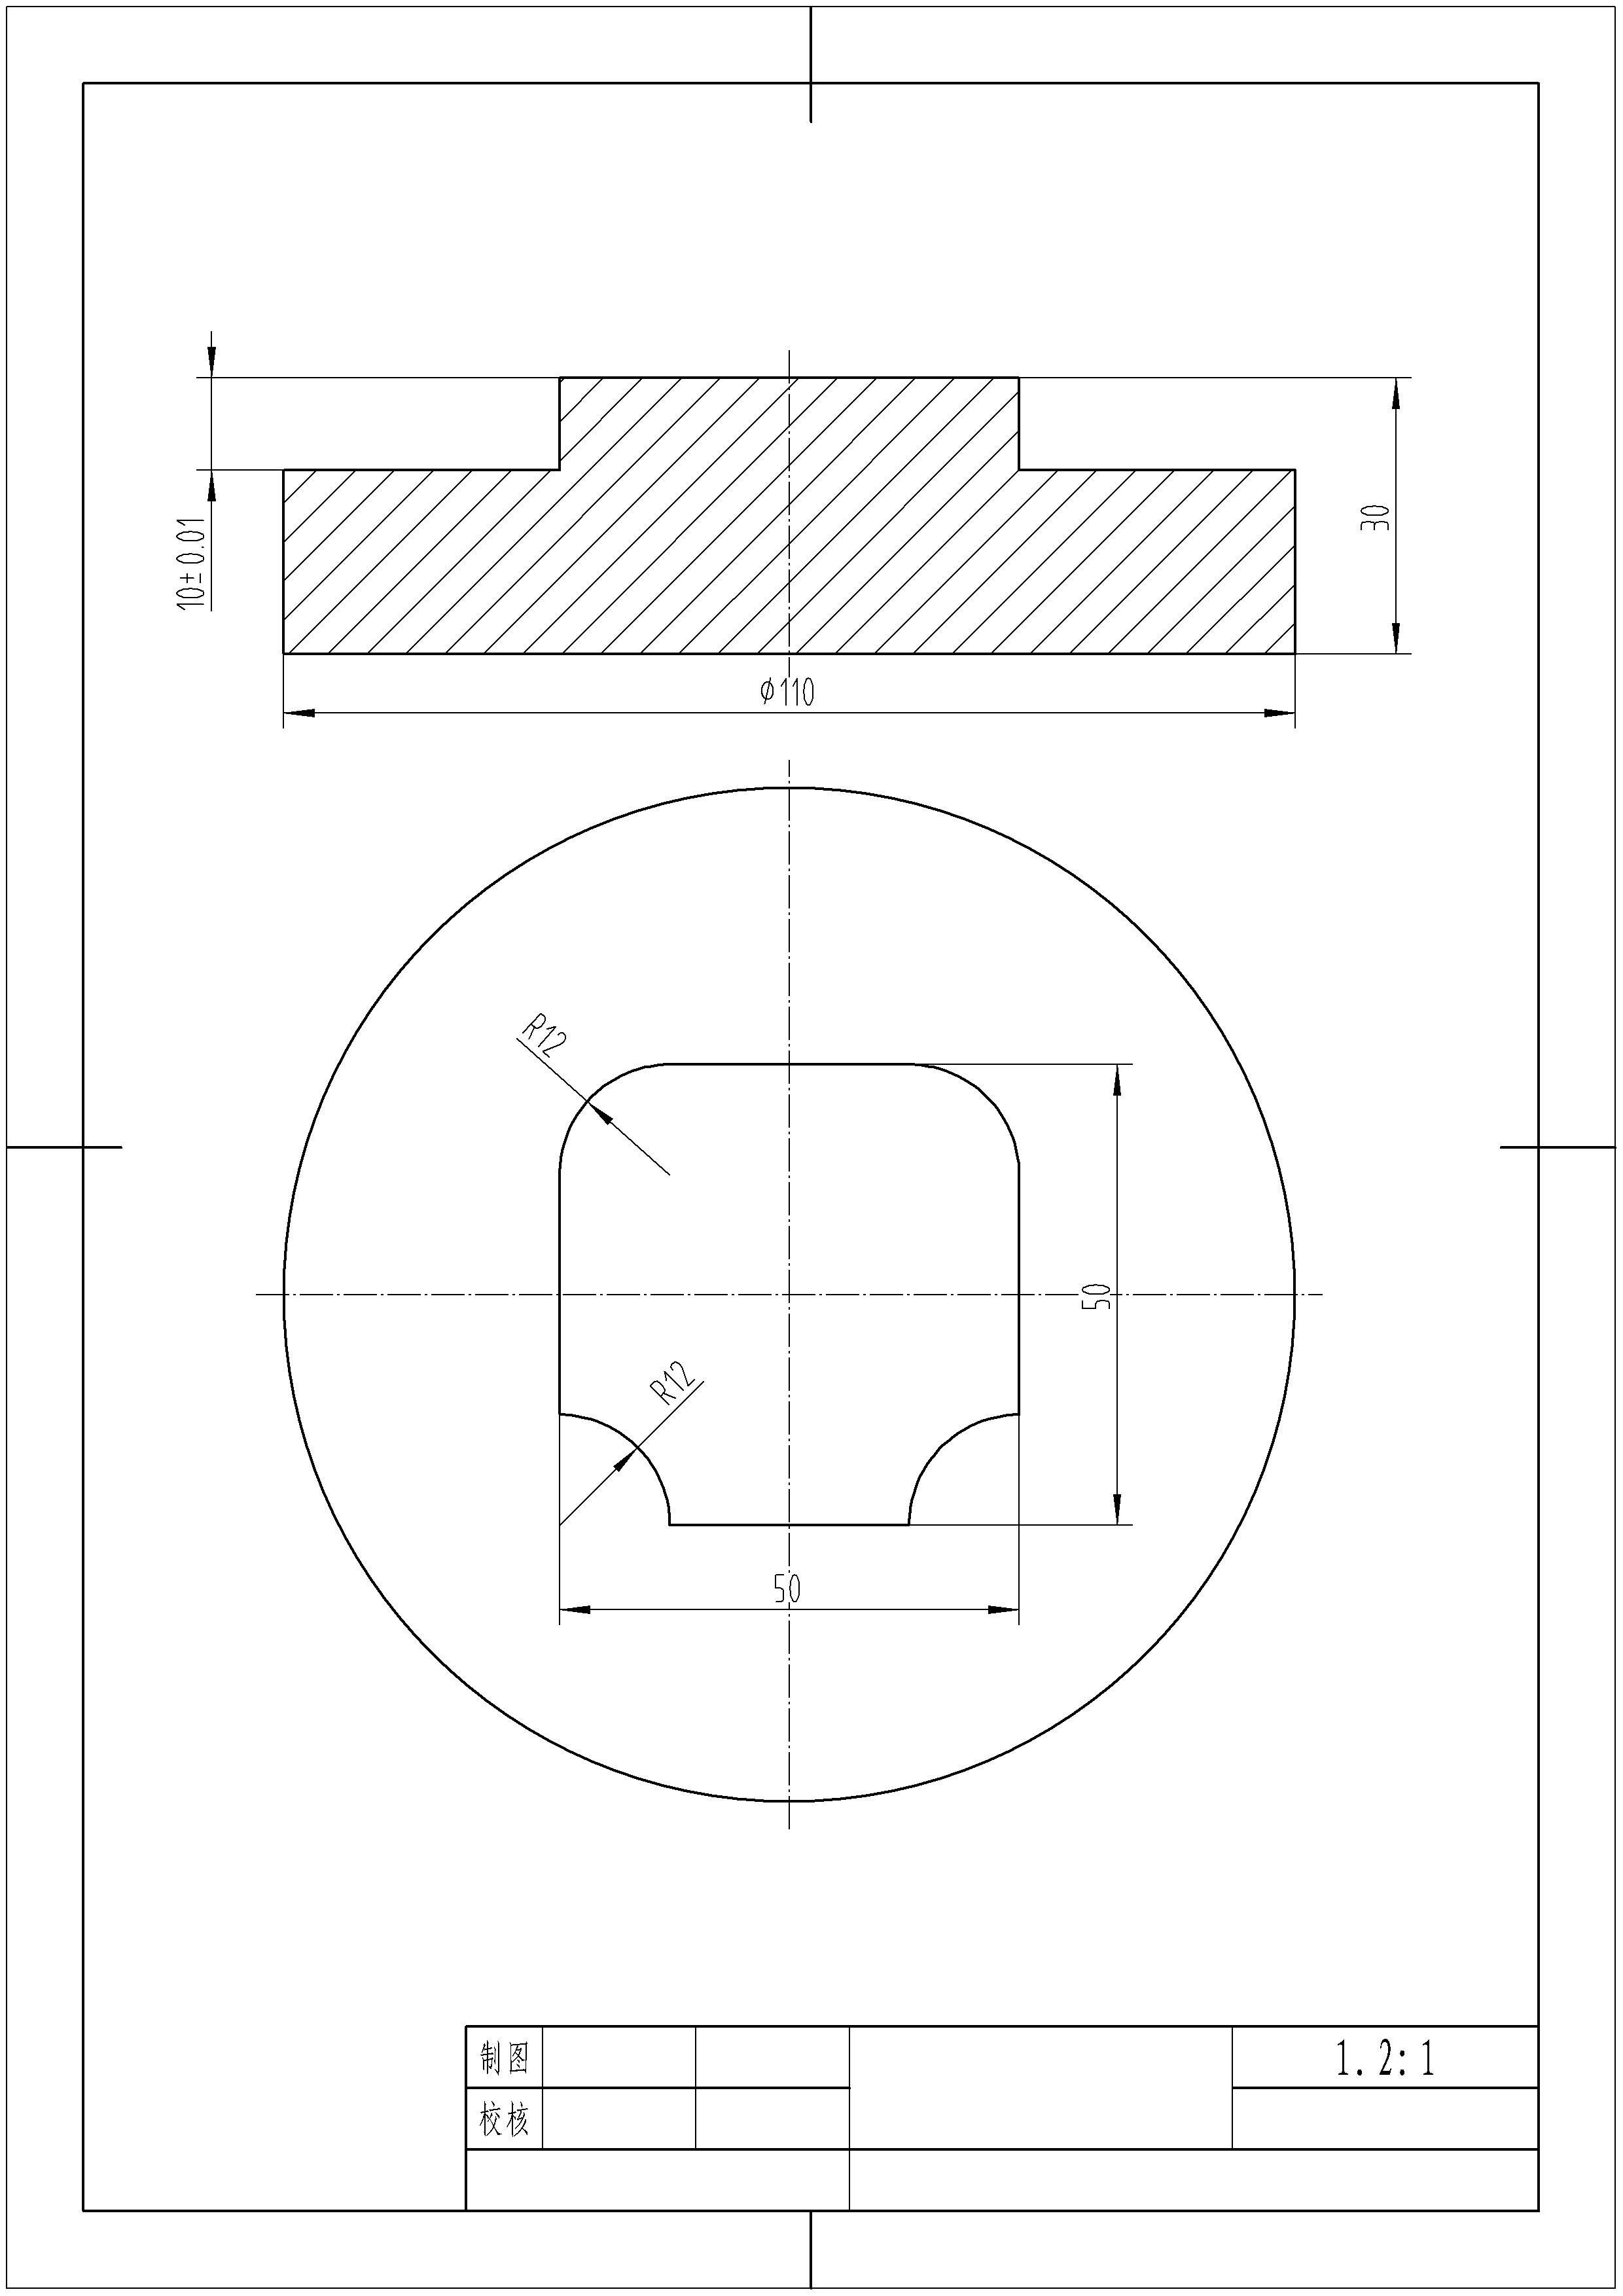
\includegraphics[width=0.8\linewidth,trim=50 150 50 100,clip]{data/image/5-1.jpg}
	\caption{}
	\label{fig:6-1}
\end{figure}

\begin{enumerate}[1、]
	\item 图样分析;
	\item 确定加工内容;
	\item 确定装夹及工件坐标系;
	\item 确定刀具及切削用量;
	\item 确定工序及走刀路线;
	\item 计算点坐标;
	\item 编写程序单。
\end{enumerate}

\subsection{教学内容及过程}

\subsubsection{案例分析}

在数控铣床或加工中心上加工如图\ref{fig:6-2}所示的零件,试完成程序的编写,已知毛坯为 $\Phi$ 110*30。

\begin{figure}[h]
	\centering
	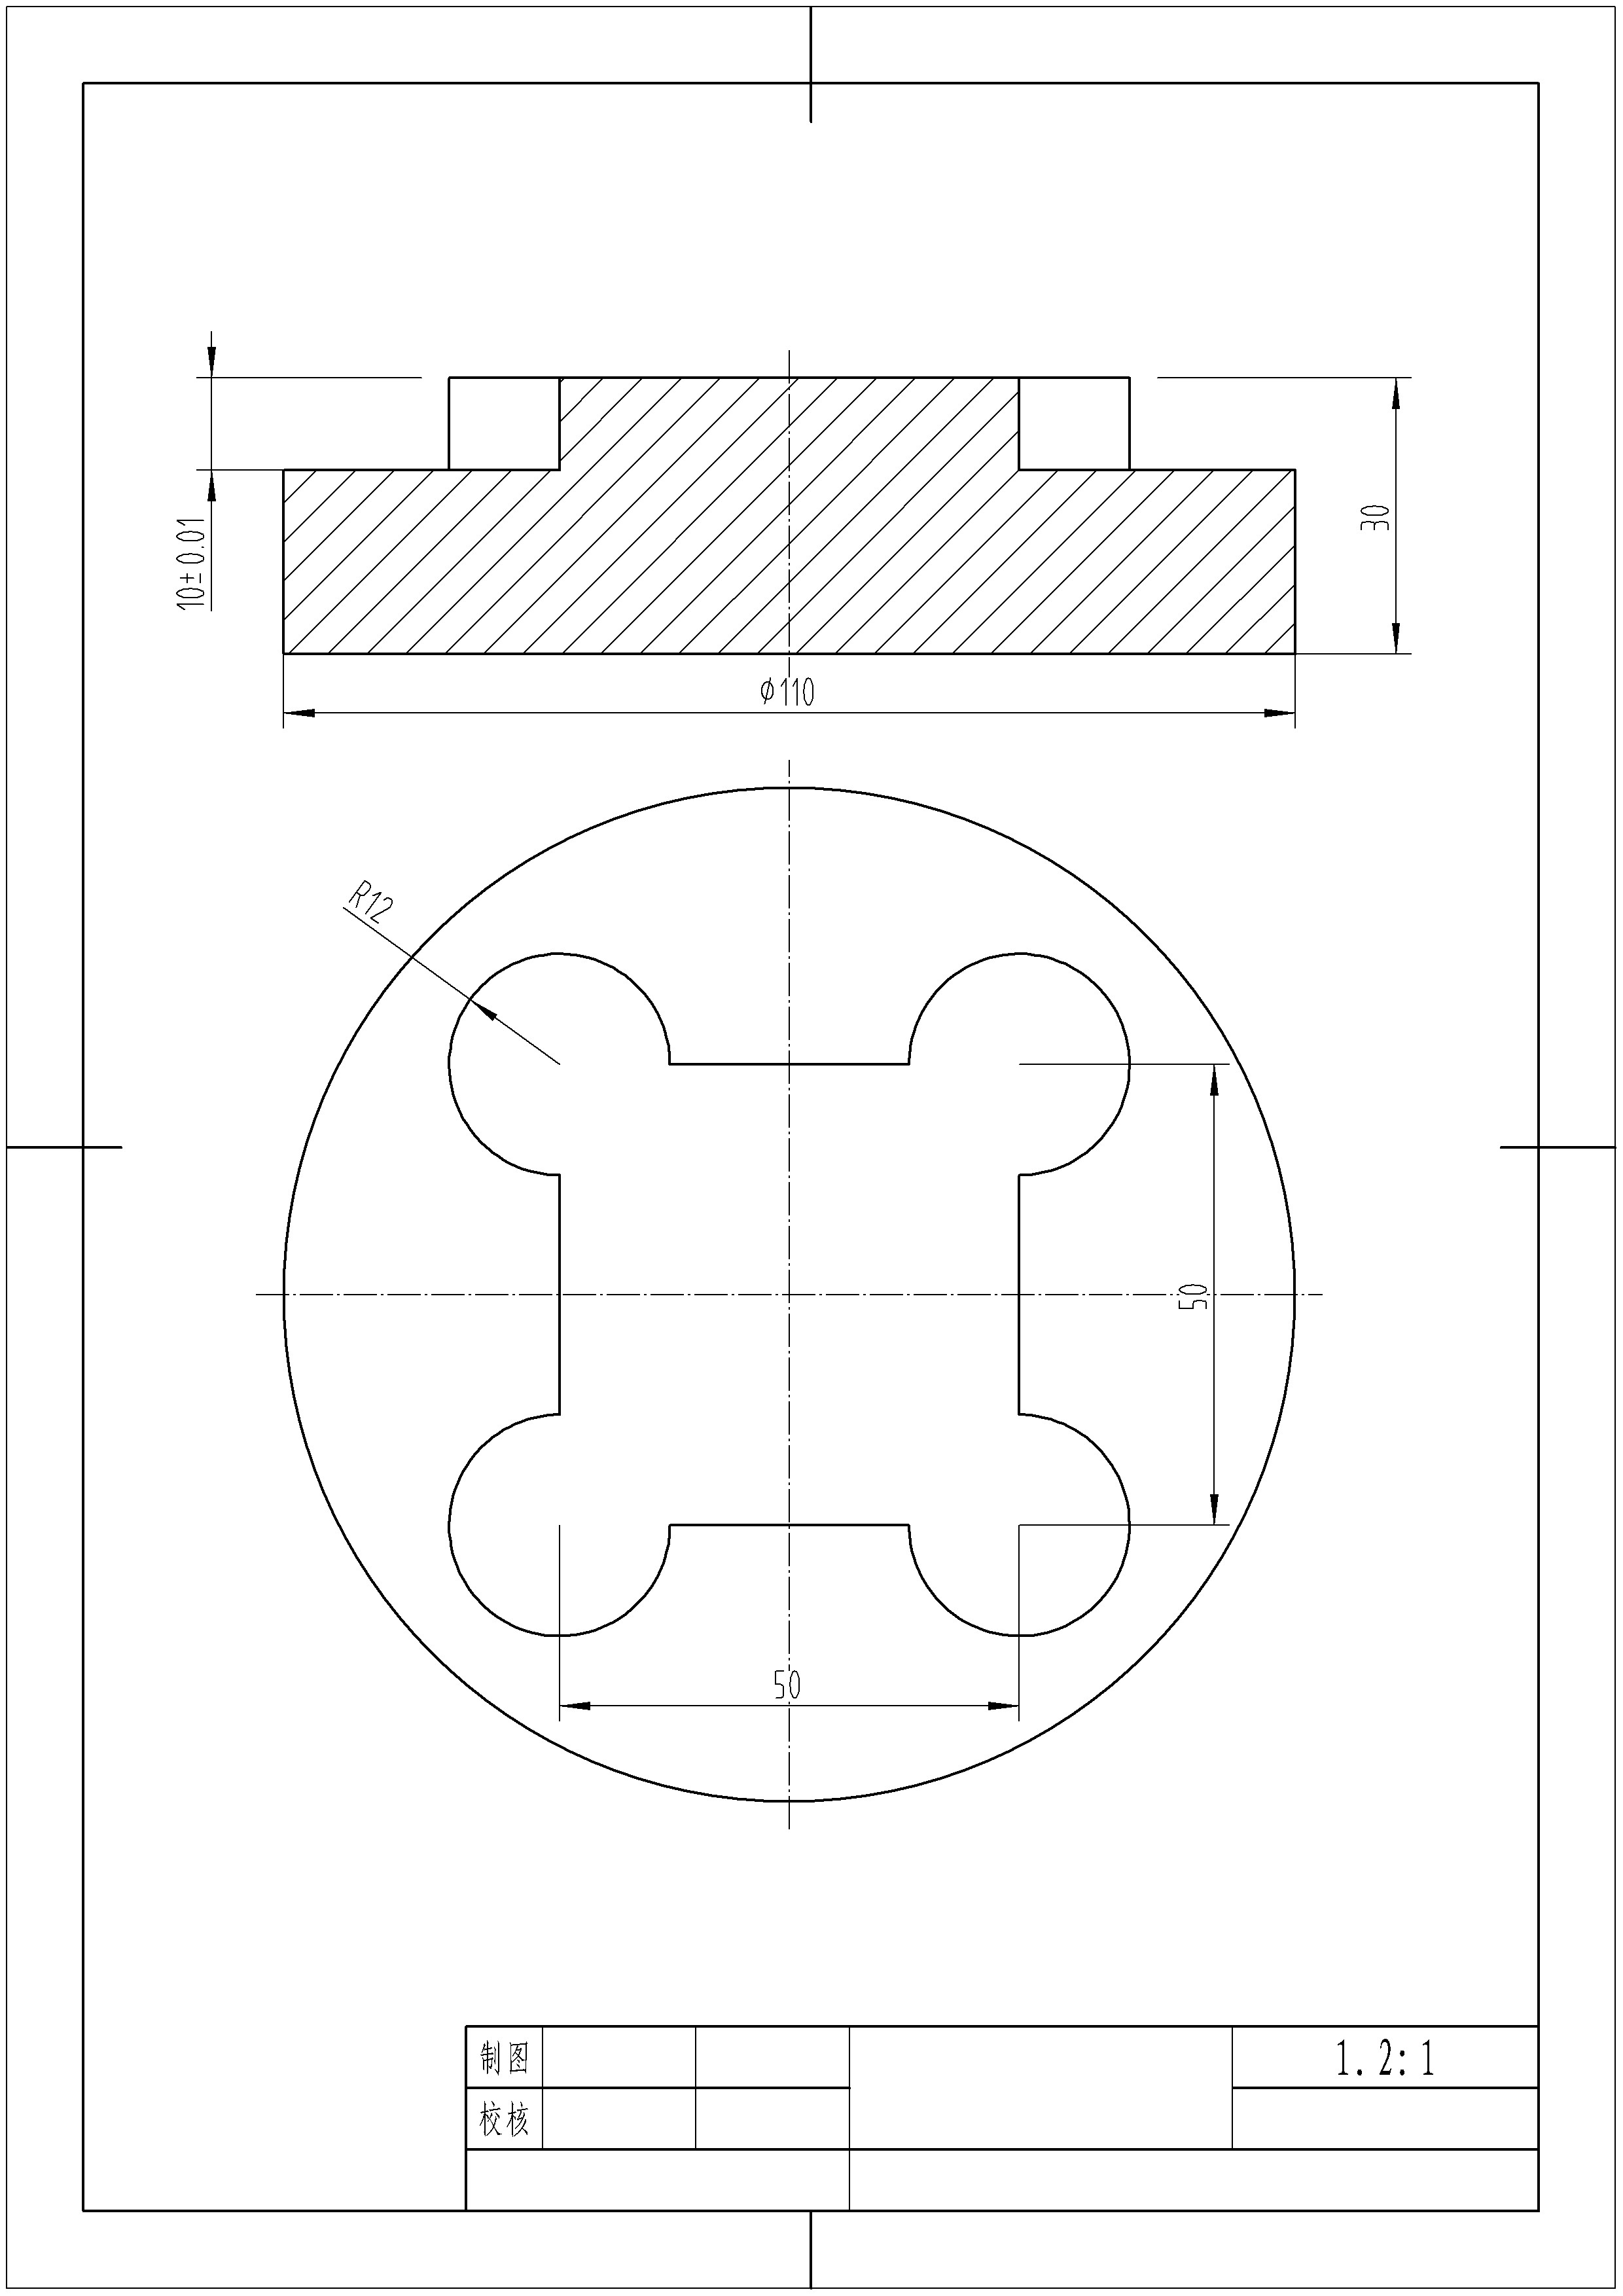
\includegraphics[width=0.8\linewidth,trim=50 150 50 100,clip]{data/image/5-2.jpg}
	\caption{}
	\label{fig:6-2}
\end{figure}

\begin{enumerate}[1、]
	\item 图样分析;
	\item 确定加工内容;
	\item 确定装夹及工件坐标系;
	\item 确定刀具及切削用量;
	\item 确定工序及走刀路线;
	\item 计算点坐标;
	\item 编写程序单。
\end{enumerate}


路径特点:

圆弧的圆心角大于180度,显然不能直接用前面的程序。

解决方法:解决方法:



1、把圆弧分成多个圆心角小于180度的圆弧。

2、掌握圆心角大于180度圆弧指令的使用。

当圆心角大于180度时,用负的半径值来表示。

当圆心角小于180度时,用正的半径值来表示。

Siemens上用CR= 正负规则一样。



\subsubsection{整圆编程}
在数控铣床或加工中心上用整圆的路径进行面铣,面铣深度为1mm,试完成加工成型的编写。
\begin{figure}[h]
	\centering
	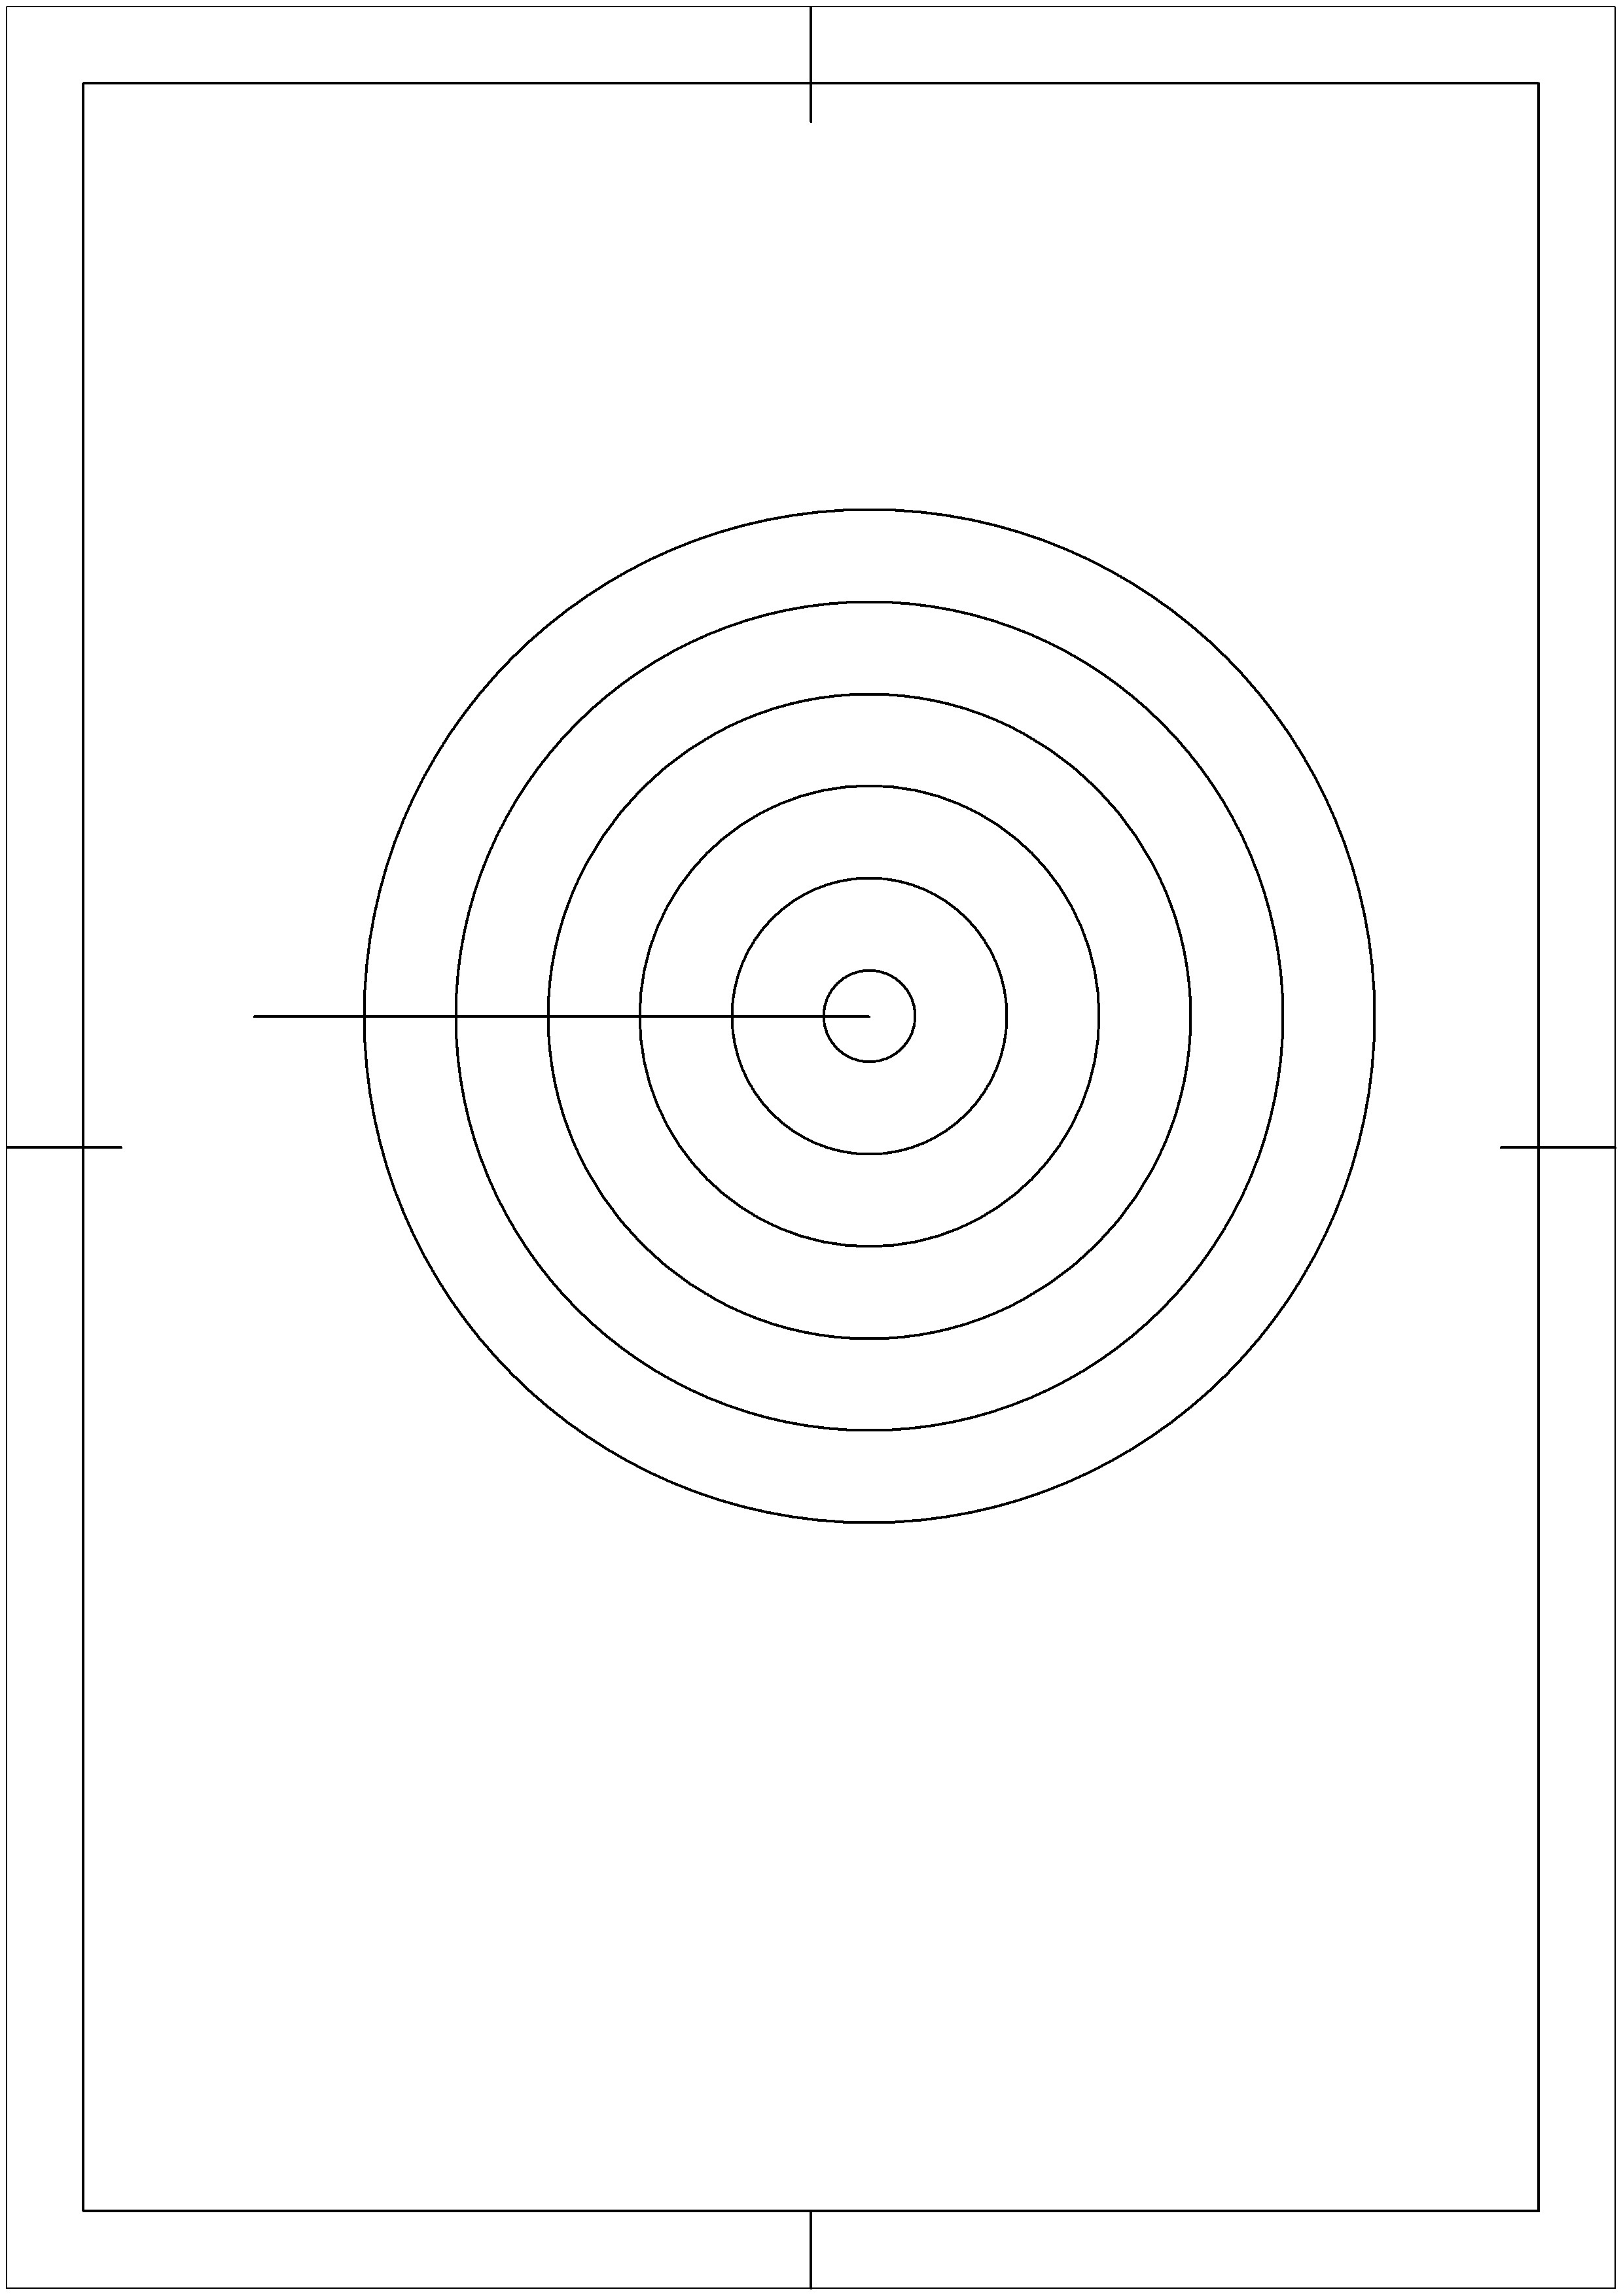
\includegraphics[width=0.8\linewidth,trim=50 150 50 100,clip]{data/image/5-3.jpg}
	\caption{}
	\label{fig:6-3}
\end{figure}

整圆路径也可以分成多个圆弧。

一个整圆路径可以用IJK圆心来编程。

不能用半径来编写一个整圆。


I、J、K表示圆心相对于起点的坐标。即:

I=X圆心-X起点

J=Y圆心-Y起点

K=Z圆心-Z起点

I、J、K与G90/G91无关,只与整圆的起点有关。

如: G17 G90 G2 X-50.0 Y-50.0 I50.0 J0;

参考程序:

\begin{lstlisting}
O0001;
G54G17G90;
M3S500;
G1Z30.0F2000;
X-65.Y0;
Z5.0;
Z-1.0F200;
X-55.0;
G2X-55.0Y0I55.0;
G1X-45.0;
G2I45.0;
G1X-35.0;
G2I-35.0;
G1X-25.0;
G2I-25.0;
G1X-15.0;
G2I-15.0;
G1X-5.0;
G2I5.0;
G1Z5.0;
Z30.0F2000;
M5;
M30;
\end{lstlisting}

\subsubsection{I、J、K的应用}
在数控铣床或加工中心上加工如图所示的零件,试用I、J、K完成程序的编写。
\begin{figure}[h]
	\centering
	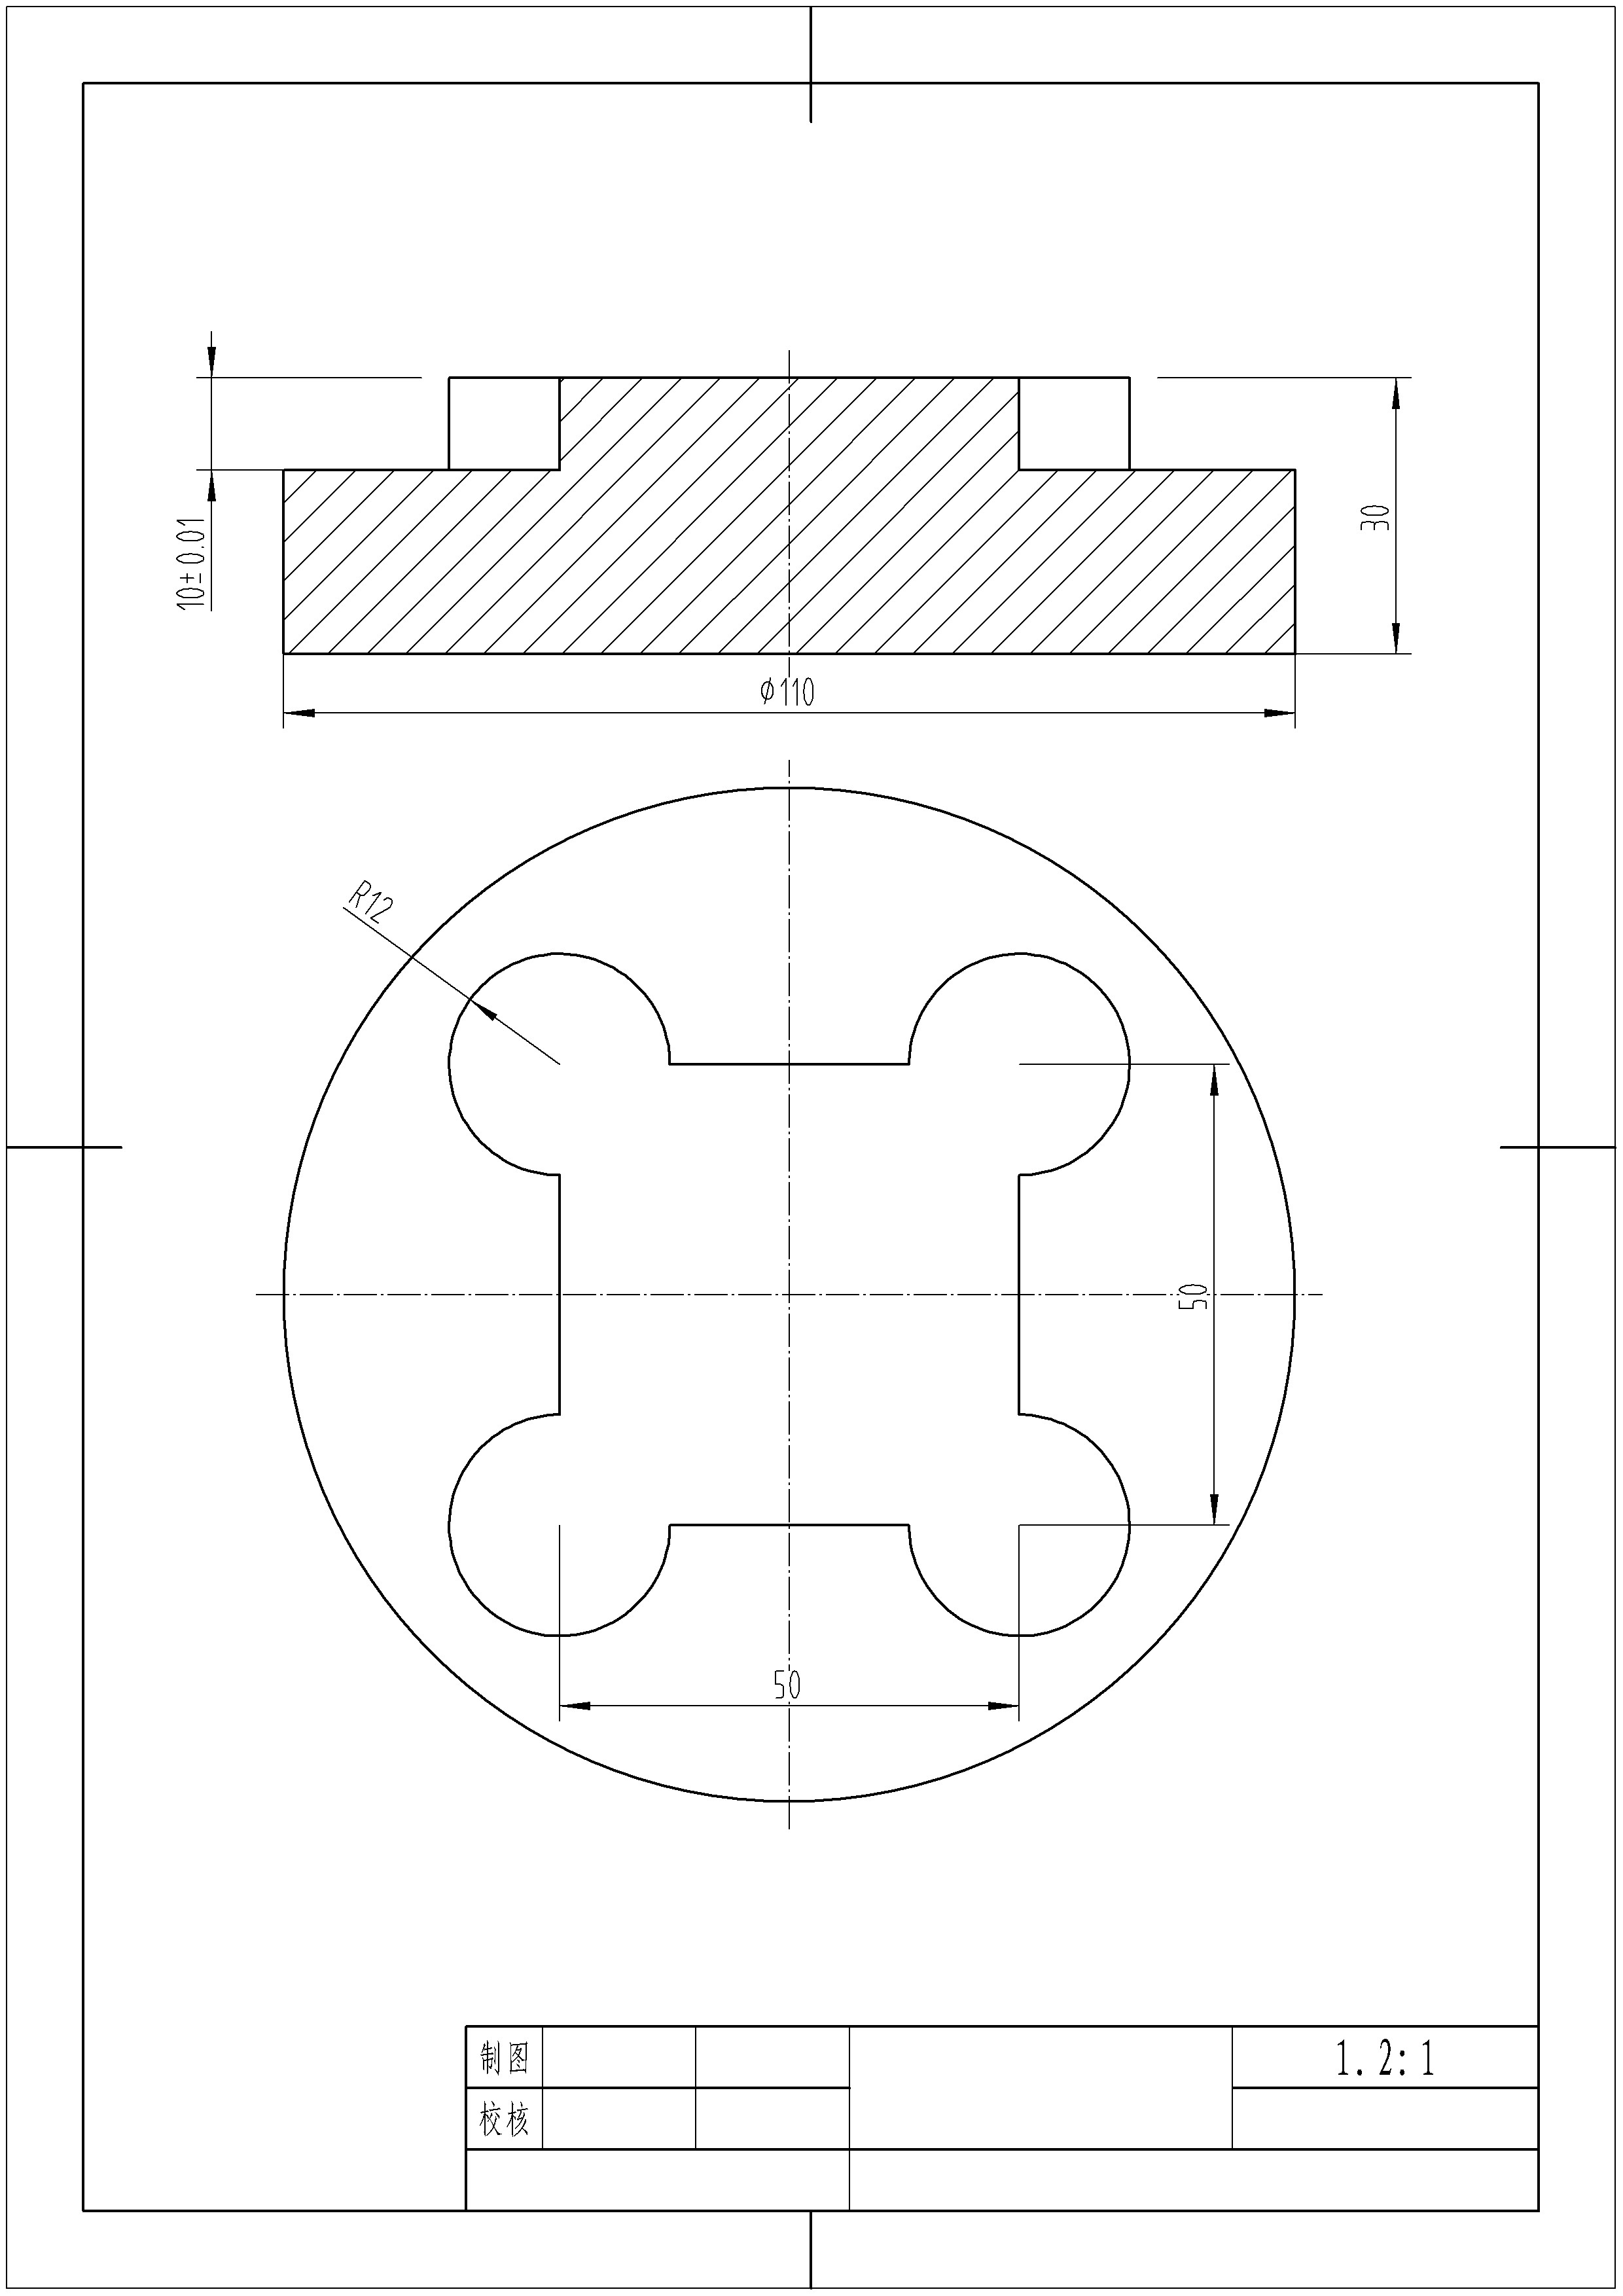
\includegraphics[width=0.8\linewidth,trim=50 150 50 100,clip]{data/image/5-4.jpg}
	\caption{}
	\label{fig:6-4}
\end{figure}
参考程序:

\begin{lstlisting}
O0001;
G54G17G90;
M3S500;
G1Z30.0F2000;
X-65.0Y0;
Z5.0;
Z-10.0F2000;
X-25.0;
Y13.0;
G2X-13.0Y25.0J13.0;
G1X13.0;
G2X25.0Y13.OJ-13.0;
….
\end{lstlisting}






手工编程中,能用半径编程就用半径编程,一般零件图标的是半径,也不容易出错。

自动编程,可以输出I、J、K以增加程序在不同机床通用性。


\subsubsection{编写程序的基本思路}
程序初始化(安全保护)--------辅助准备(换刀,主轴启动,切削液开)--------定位到起刀点--------快速下刀--------工进下刀--------走加工轮廓--------提刀---------快速提刀到安全平面-------程序结束(换刀,主轴停止,切削液关,程序返回等)
\subsection{课堂小结}
\begin{enumerate}[1、]
	\item 案例分析;
	\item 指令讲解;
	\item 编写程序;
	\item 编写程序的基本思路。
\end{enumerate}
\vfill
\subsection{布置作业}
\begin{enumerate}[1、]
	\item 自定尺寸,编写加工一个矩形外形的程序?
\end{enumerate}
\vfill
\jxhj{%教学后记
	}
\skrq{%授课日期
	2017年9月28日 4-5节}
\ktmq{%课题名称
	刀具半径补偿 }
\jxmb{%教学目标,每行前面要加 \item
	\item 了解补偿的意义;
	\item 掌握G41/G42刀具半径补偿指令的使用;
	\item 会用G41/G42刀具半径指令编写程序;
	\item 了解常用切入切出的方法。
}
\jxzd{%教学重点,每行前面要加 \item
	\item 掌握G41/G42刀具半径补偿指令的使用;
	\item 会用G41/G42刀具半径指令编写程序;}
\jxnd{%教学难点,每行前面要加 \item
	\item 会用G41/G42刀具半径指令编写程序;}
\jjff{%教学方法
	通过讲述、举例、演示法来说明;}

\makeshouye %制作教案首页

%%%%教学内容
\subsection{组织教学}
\begin{enumerate}[1、]
	\item 集中学生注意力;
	\item 清查学生人数;
	\item 维持课堂纪律;
\end{enumerate}
\subsection{复习导入及主要内容}
\begin{enumerate}[1、]
\item 在数控铣床或加工中心上加工如图所示的零件,试完成程序的编写。(试用I、J、K编写,凸台高5mm)

\begin{figure}[h]
	\centering
	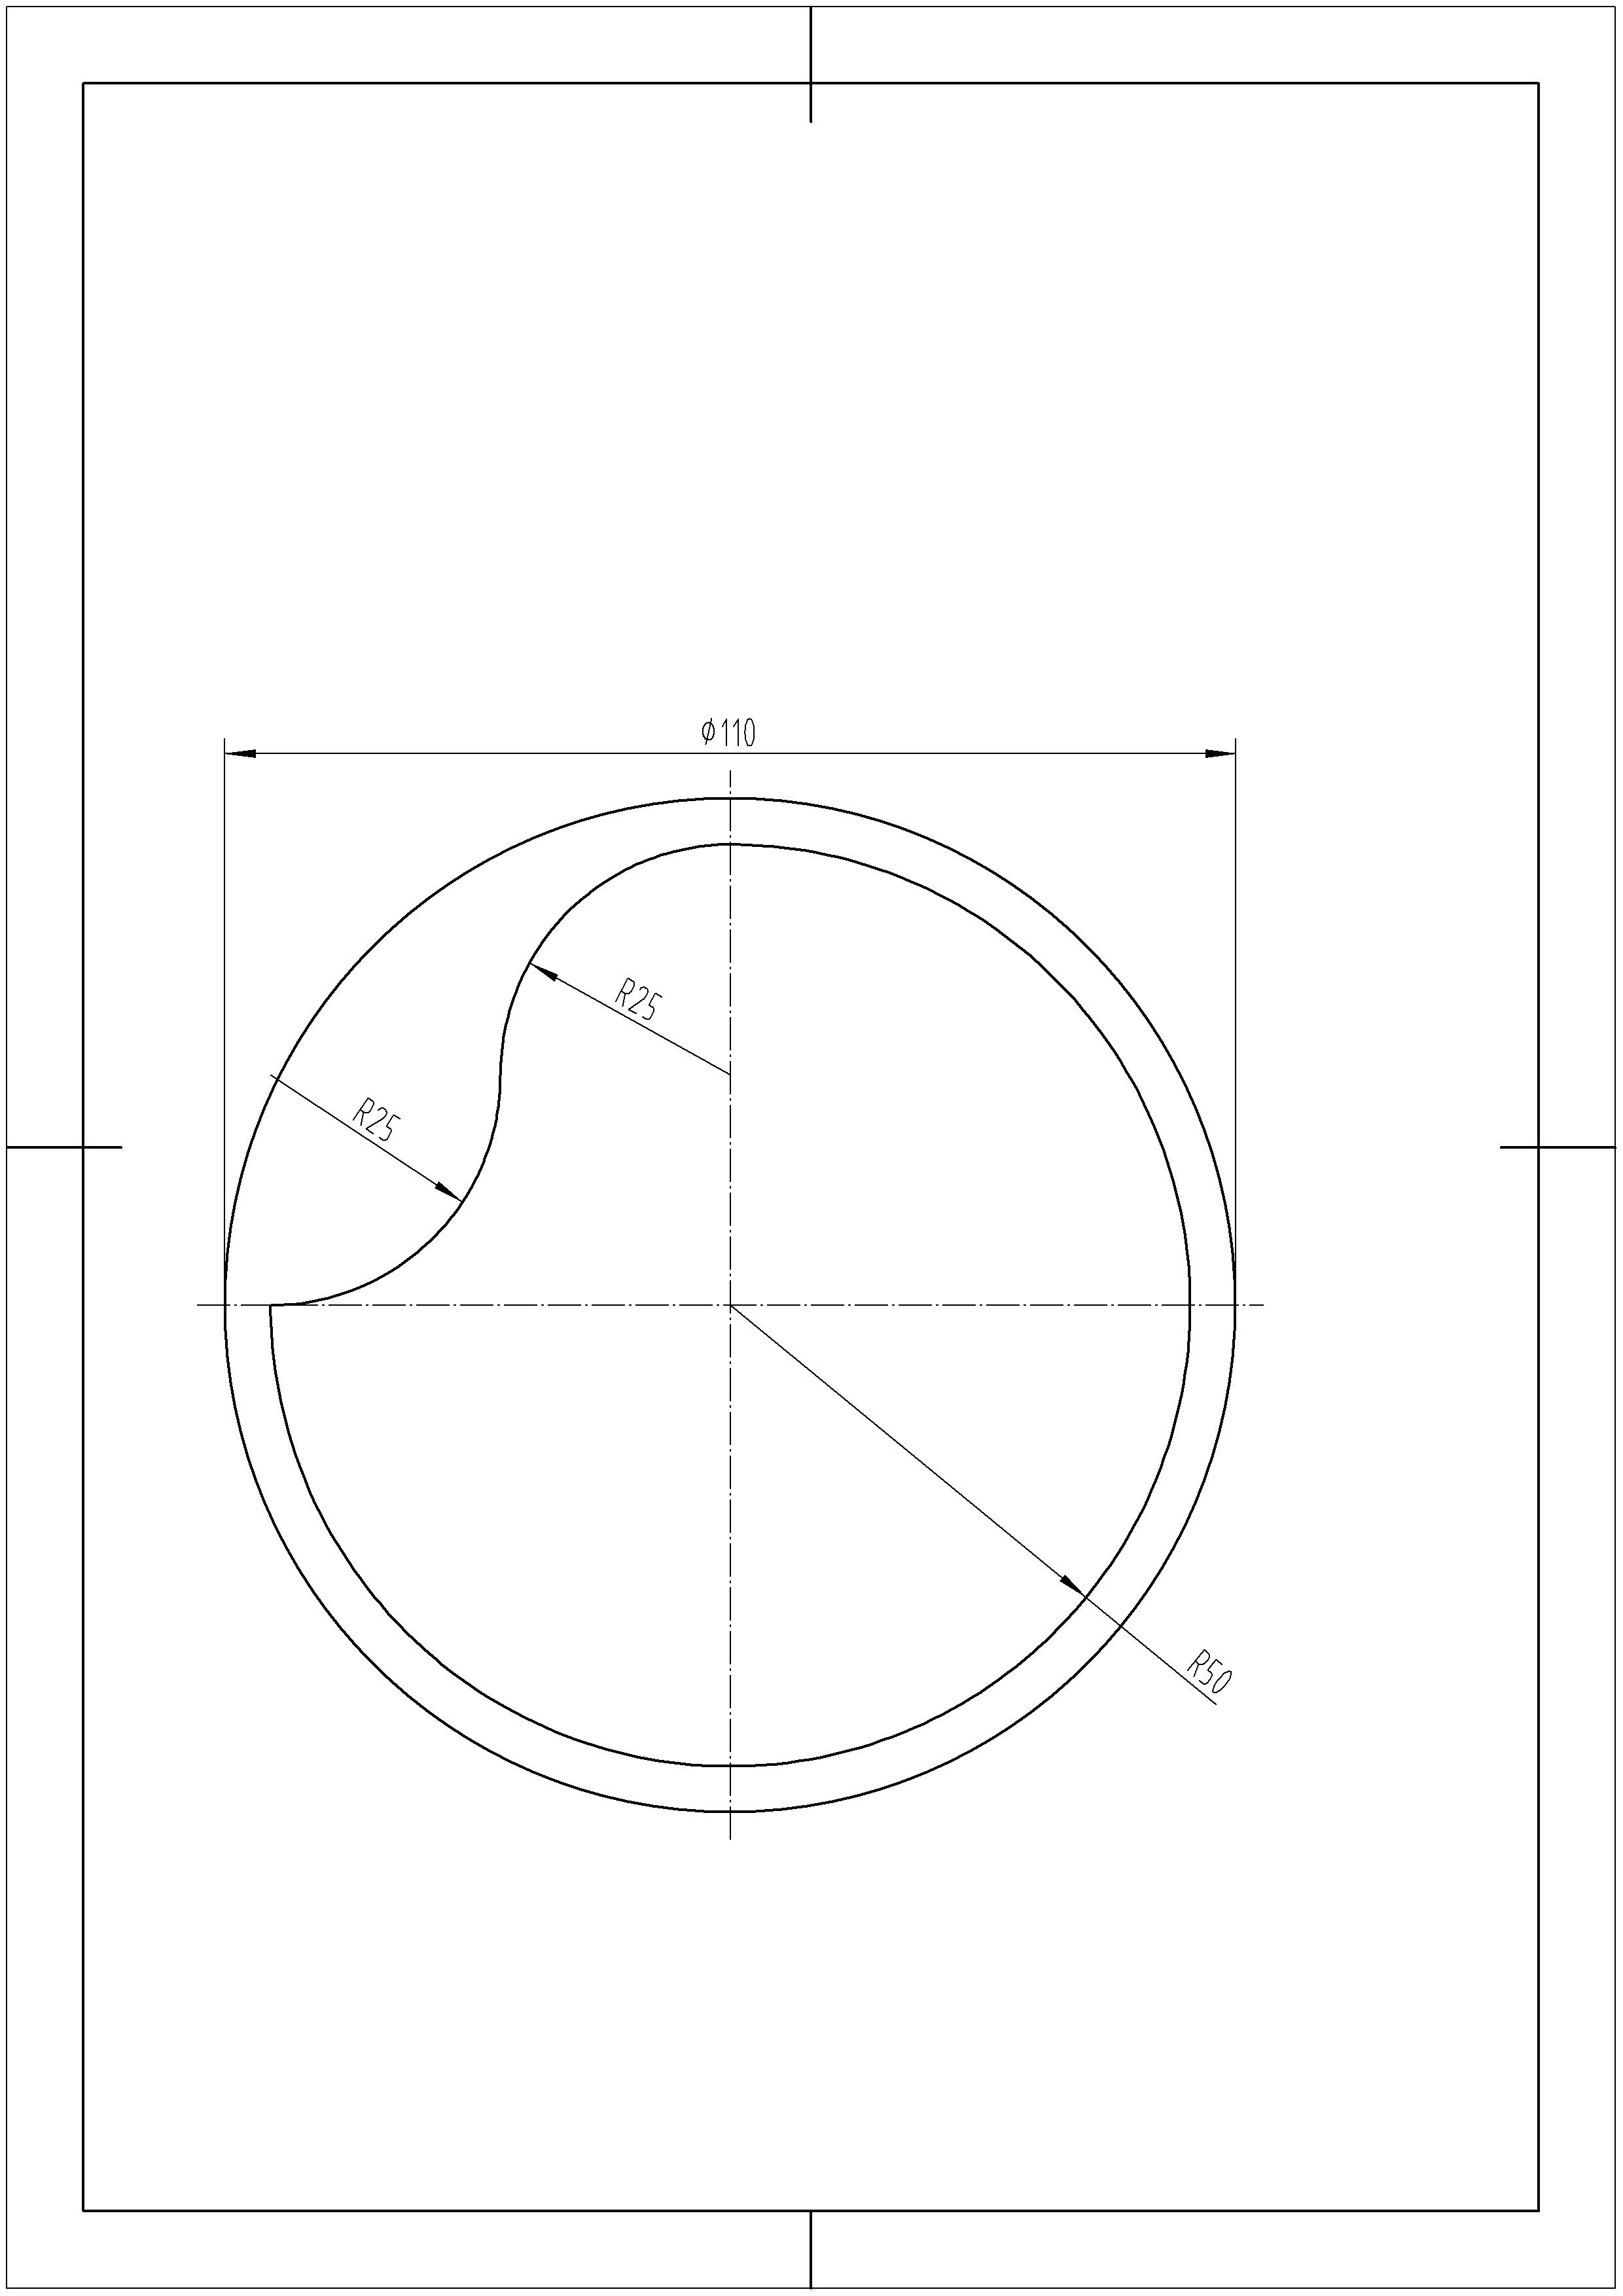
\includegraphics[width=0.8\linewidth,trim=40 150 70 220,clip]{data/image/7-1.jpg}
	\caption{复习题}
	\label{fig:7-1}
\end{figure}

\item G2/G3指令半径编程;
\item G2/G3指令圆心编程;
\item 编写程序的基本思路。
\end{enumerate}

\subsection{教学内容及过程}

\subsubsection{加工尺寸的分析}

由于加工刀具存在一个尺寸,故加工出来的尺寸值会每边少一个刀具半径。

解决方法:

1、更改加工刀路,使其偏移一个刀具半径(粗加工及去残料)。

2、使用刀具半径补偿指令进行编程。

例子:

\begin{lstlisting}
O0001;
G54G71G40G90;
M3S500;
G1Z30.F200O;
X70.YO;
Z5.;
Z-5.F200;
X66.Y10.;
G3X56.Y0R10.;
G2X-56.I-56.;
G2X-50.Y6.0.I6.0;(中间的过度)
G3X-31.Y25.J19.;
G2X0Y56.I31.;
X56.YOJ-56.;
G3X66.Y-10.I10.;
G1Z5.0;
Z30.F2000;
M5;
M30;
\end{lstlisting}
(麻烦,但有时必须这么做)


\subsubsection{刀具半径补偿}

由CNC系统内部使刀具在加工时,自动偏移一个刀具半径。
简化编程的难度。

指令G40、G41/G42

1、补偿方向的确定:

ISO 标准规定,当刀具中心轨迹在编程轨迹前进方向的左边时,称为左刀补,用G41表示;刀具中心轨迹在编程轨迹前进方向的右边时,称为右刀补,用G42表示;注销刀具半径补偿时用G40表示。

\begin{figure}[h]
	\centering
    
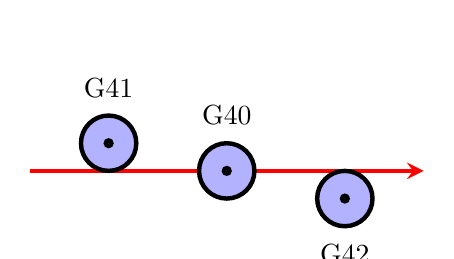
\begin{tikzpicture}[ultra thick]
\draw[->,red,>=stealth]  (0,0) -- (5,0);
\draw[fill=blue!30] (1,10pt) circle (10pt) circle (1pt);
\draw[fill=blue!30] (2.5,0) circle (10pt) circle (1pt);
\draw[fill=blue!30] (4,-10pt) circle (10pt) circle (1pt);
\node at (1,30pt) {G41};
\node at (2.5,20pt) {G40};
\node at (4,-30pt) {G42};
\end{tikzpicture}

\caption{刀补位置}
\label{fig:7-5}
\end{figure}

2、补偿值的设定:

通过参数进行设定:

[OfFset]---[补偿]----[位置号]----[D形状+D磨shen损]

3、指令的格式:

在开始刀补的位置,结合G1指令设定补偿方向及补偿值位置号,在结束的位置,用G40结合G1指令即可:

G41/G42 G1 X\_ Y\_  D\_;

……

G40 G1 X\_ Y\_;

4、补偿平面

可以在G18及G19平面上进行刀具半径补偿,(常用于球头刀)

5、补偿过程分析:

1)刀具半径补偿建立:当输入BS缓冲器的程序段包含有G41/G42命令时,系统认为此时已进入刀补建立状态。当以下条件成立时,加工中心以移动坐标轴的形式开始补偿动作。 

a. 有G41或G42被指定; 

b. 在补偿平面内有轴的移动; 

c. 指定了一个补偿号或已经指定一个补偿号但不能是D00;
 
d. 偏置(补偿)平面被指定或已经被指定; 

e. G00或G01模式有效。 

2) 补偿模式:在刀具补偿进行期间,刀具中心轨迹始终偏离编程轨迹一个刀具半径值的距离。此时半径补偿在G00、G01、G02、G03情况下均有效。 

3) 取消补偿:使用G40指令消去程序段偏置值,使刀具撤离工件,回到起始位置,从而使刀具中心与偏程轨迹重合。当以下两种情况之一发生时加工中心补偿模式被取消。

①给出G40同时要有补偿平面内坐标轴移动。

②刀具补偿号为D00。

4)不同平面内的半径补偿 

刀具半径补偿用G17、G18、G19命令在被选择的工作平面内进行补偿。即当G18命令执行后,刀具半径补偿仅影响X、Z移动,而对Y轴没有作用。


\subsubsection{注意事项}
1、G41/G42必须与G1/G0结合使用,不可在G2/G3圆弧指令下使用。

2、刀具必须在加工平面内有移动。

3、使用与取消必须成对使用。

4、加工前必须设定其补偿值。

5、切入前指定、切出后取消。


\subsubsection{编程实例}
1、在数控铣床或加工中心上加工如图\ref{fig:7-2}所示的零件,试完成程序的编写。
\begin{figure}[h]
	\centering
	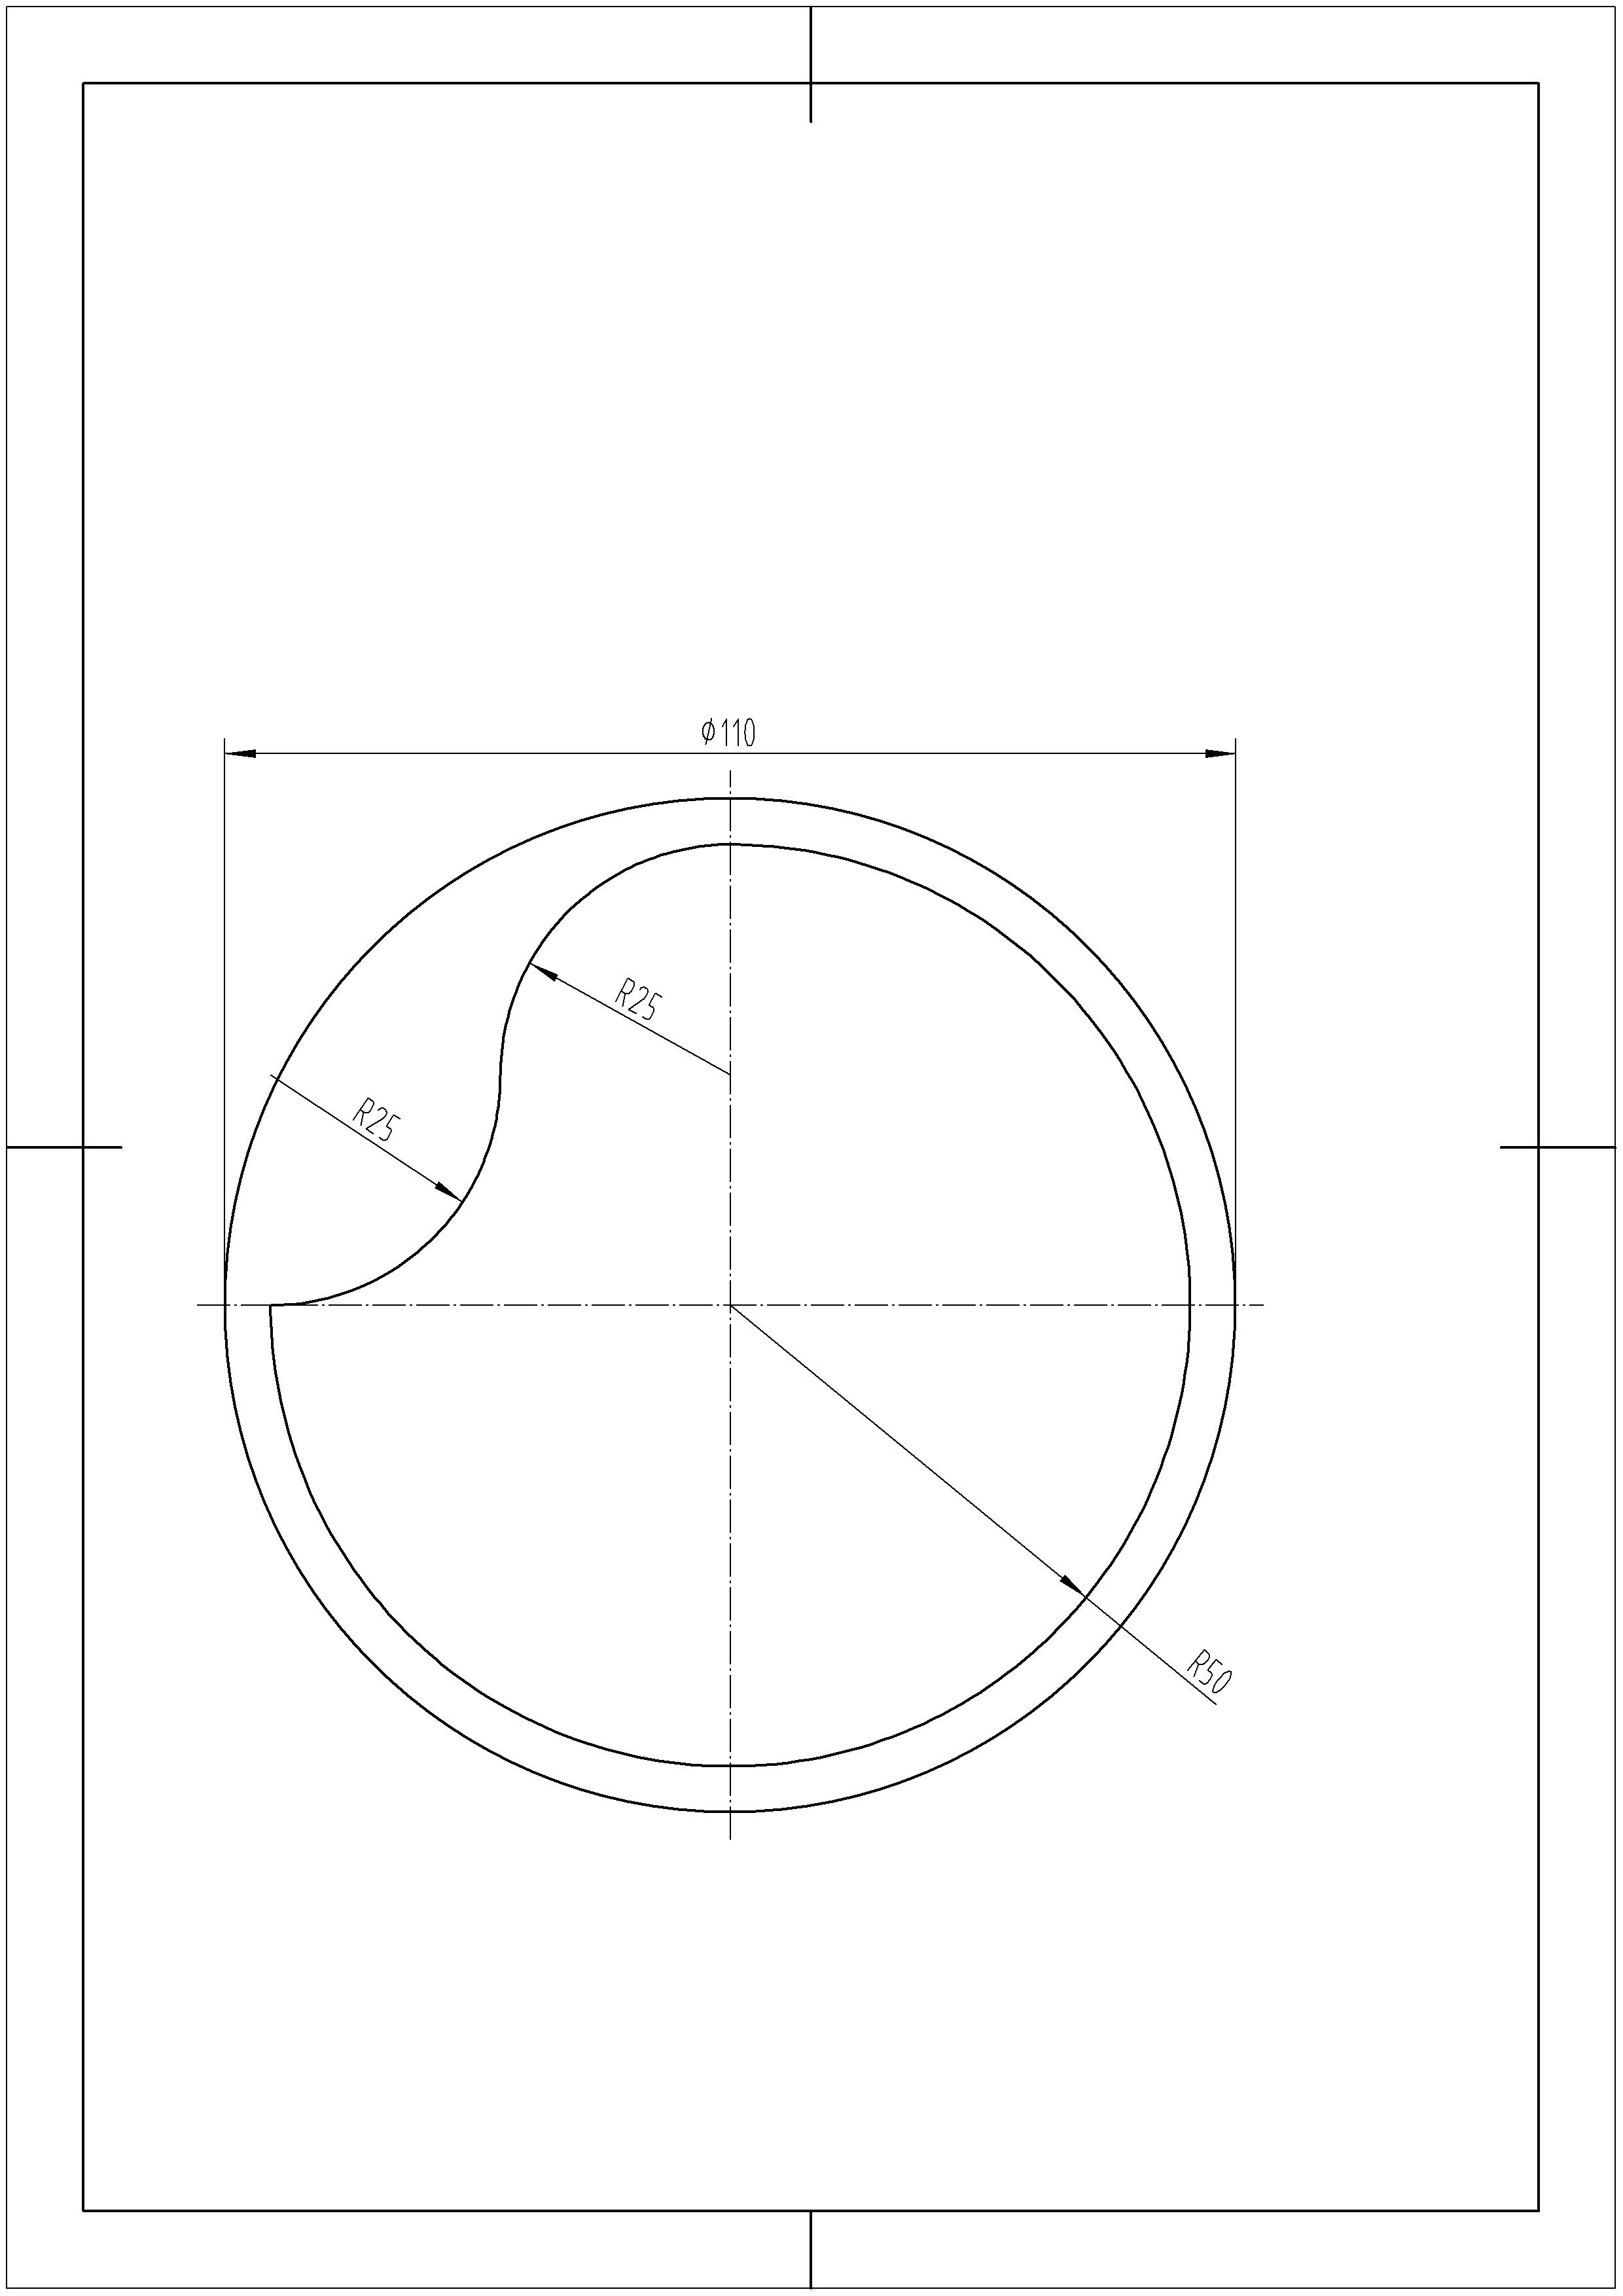
\includegraphics[width=0.8\linewidth,trim=40 150 70 220,clip]{data/image/7-1.jpg}
	\caption{刀补实例1}
	\label{fig:7-2}
\end{figure}

2、在数控铣床或加工中心上加工如图\ref{fig:7-3}所示的零件,试完成程序的编写。

\begin{figure}[h]
	\centering
	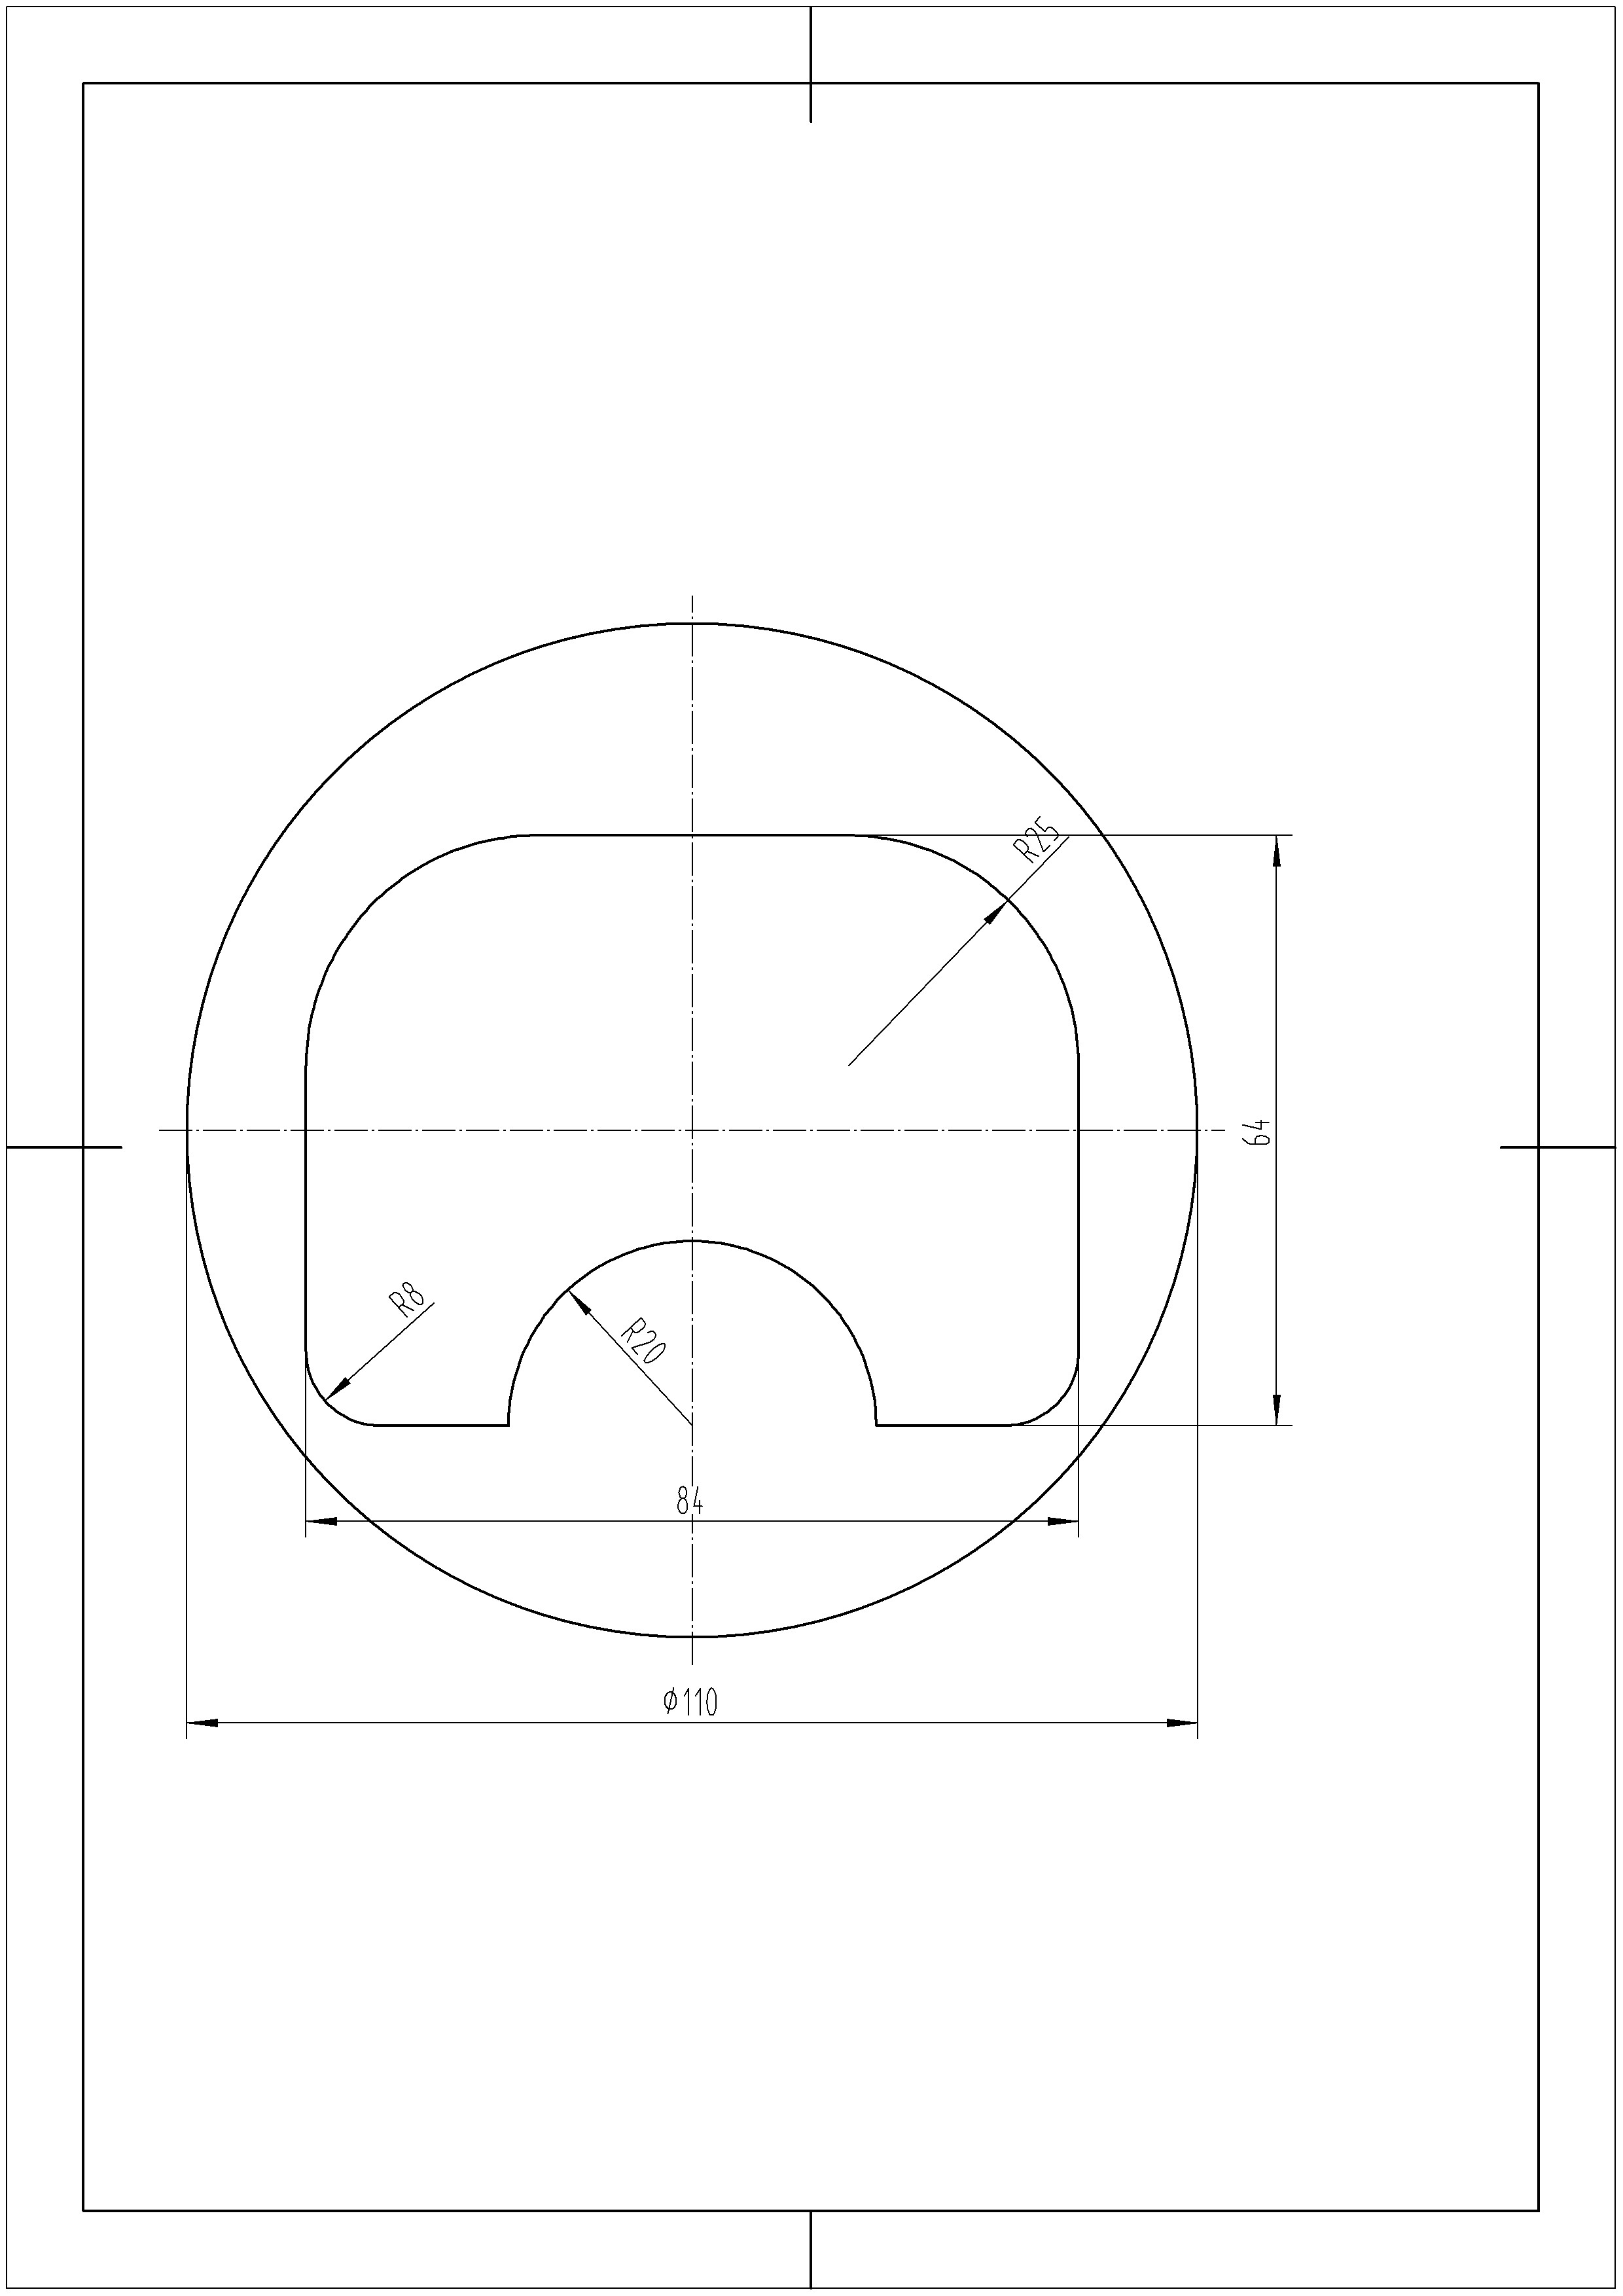
\includegraphics[width=0.8\linewidth,trim=40 150 70 220,clip]{data/image/7-2.jpg}
	\caption{刀补实例2}
	\label{fig:7-3}
\end{figure}


\subsection{课堂小结}
\begin{enumerate}[1、]
\item 刀补的概念
\item G40、G41/G42指令的使用;
\item 注意事项;
\item 刀补的编程;
\end{enumerate}

\vfill
\subsection{布置作业}
\begin{enumerate}[1、]
	\item 写出上面的程序。
	\item 习题集。
\end{enumerate}
\vfill
\jxhj{%教学后记
	}
\skrq{%授课日期
	2017年10月10日 4-5节}
\ktmq{%课题名称
	 刀具半径补偿的应用(一)}
\jxmb{%教学目标,每行前面要加 \item
	\item 掌握用刀补进行精加工;
	\item 掌握刀补值的计算;
	\item 会用G41/G42刀具半径指令编写程序;
	\item 了解常用切入切出的方法。
 }
\jxzd{%教学重点,每行前面要加 \item
	\item 用刀补进行精加工;
	\item 刀补值的计算。 }
\jxnd{%教学难点,每行前面要加 \item
	\item 刀补值的计算。 }
\jjff{%教学方法
	通过讲述、举例、演示、分析法来说明;}

\makeshouye %制作教案首页

%%%%教学内容
\subsection{组织教学}
\begin{enumerate}[\hspace{2em}1、]
	\item 集中学生注意力;
	\item 清查学生人数;
	\item 维持课堂纪律;
\end{enumerate}
\subsection{复习导入及主要内容}
\begin{enumerate}[1、]
\item 刀补的概念
\item G40、G41/G42指令的使用;
\item 注意事项;
\item 刀补的编程;
\item 在数控铣床或加工中心上加工如图\ref{fig:8-1}所示的零件,试完成程序的编写。(试用I、J、K编写,凸台高5mm)

\begin{figure}[h]
	\centering
	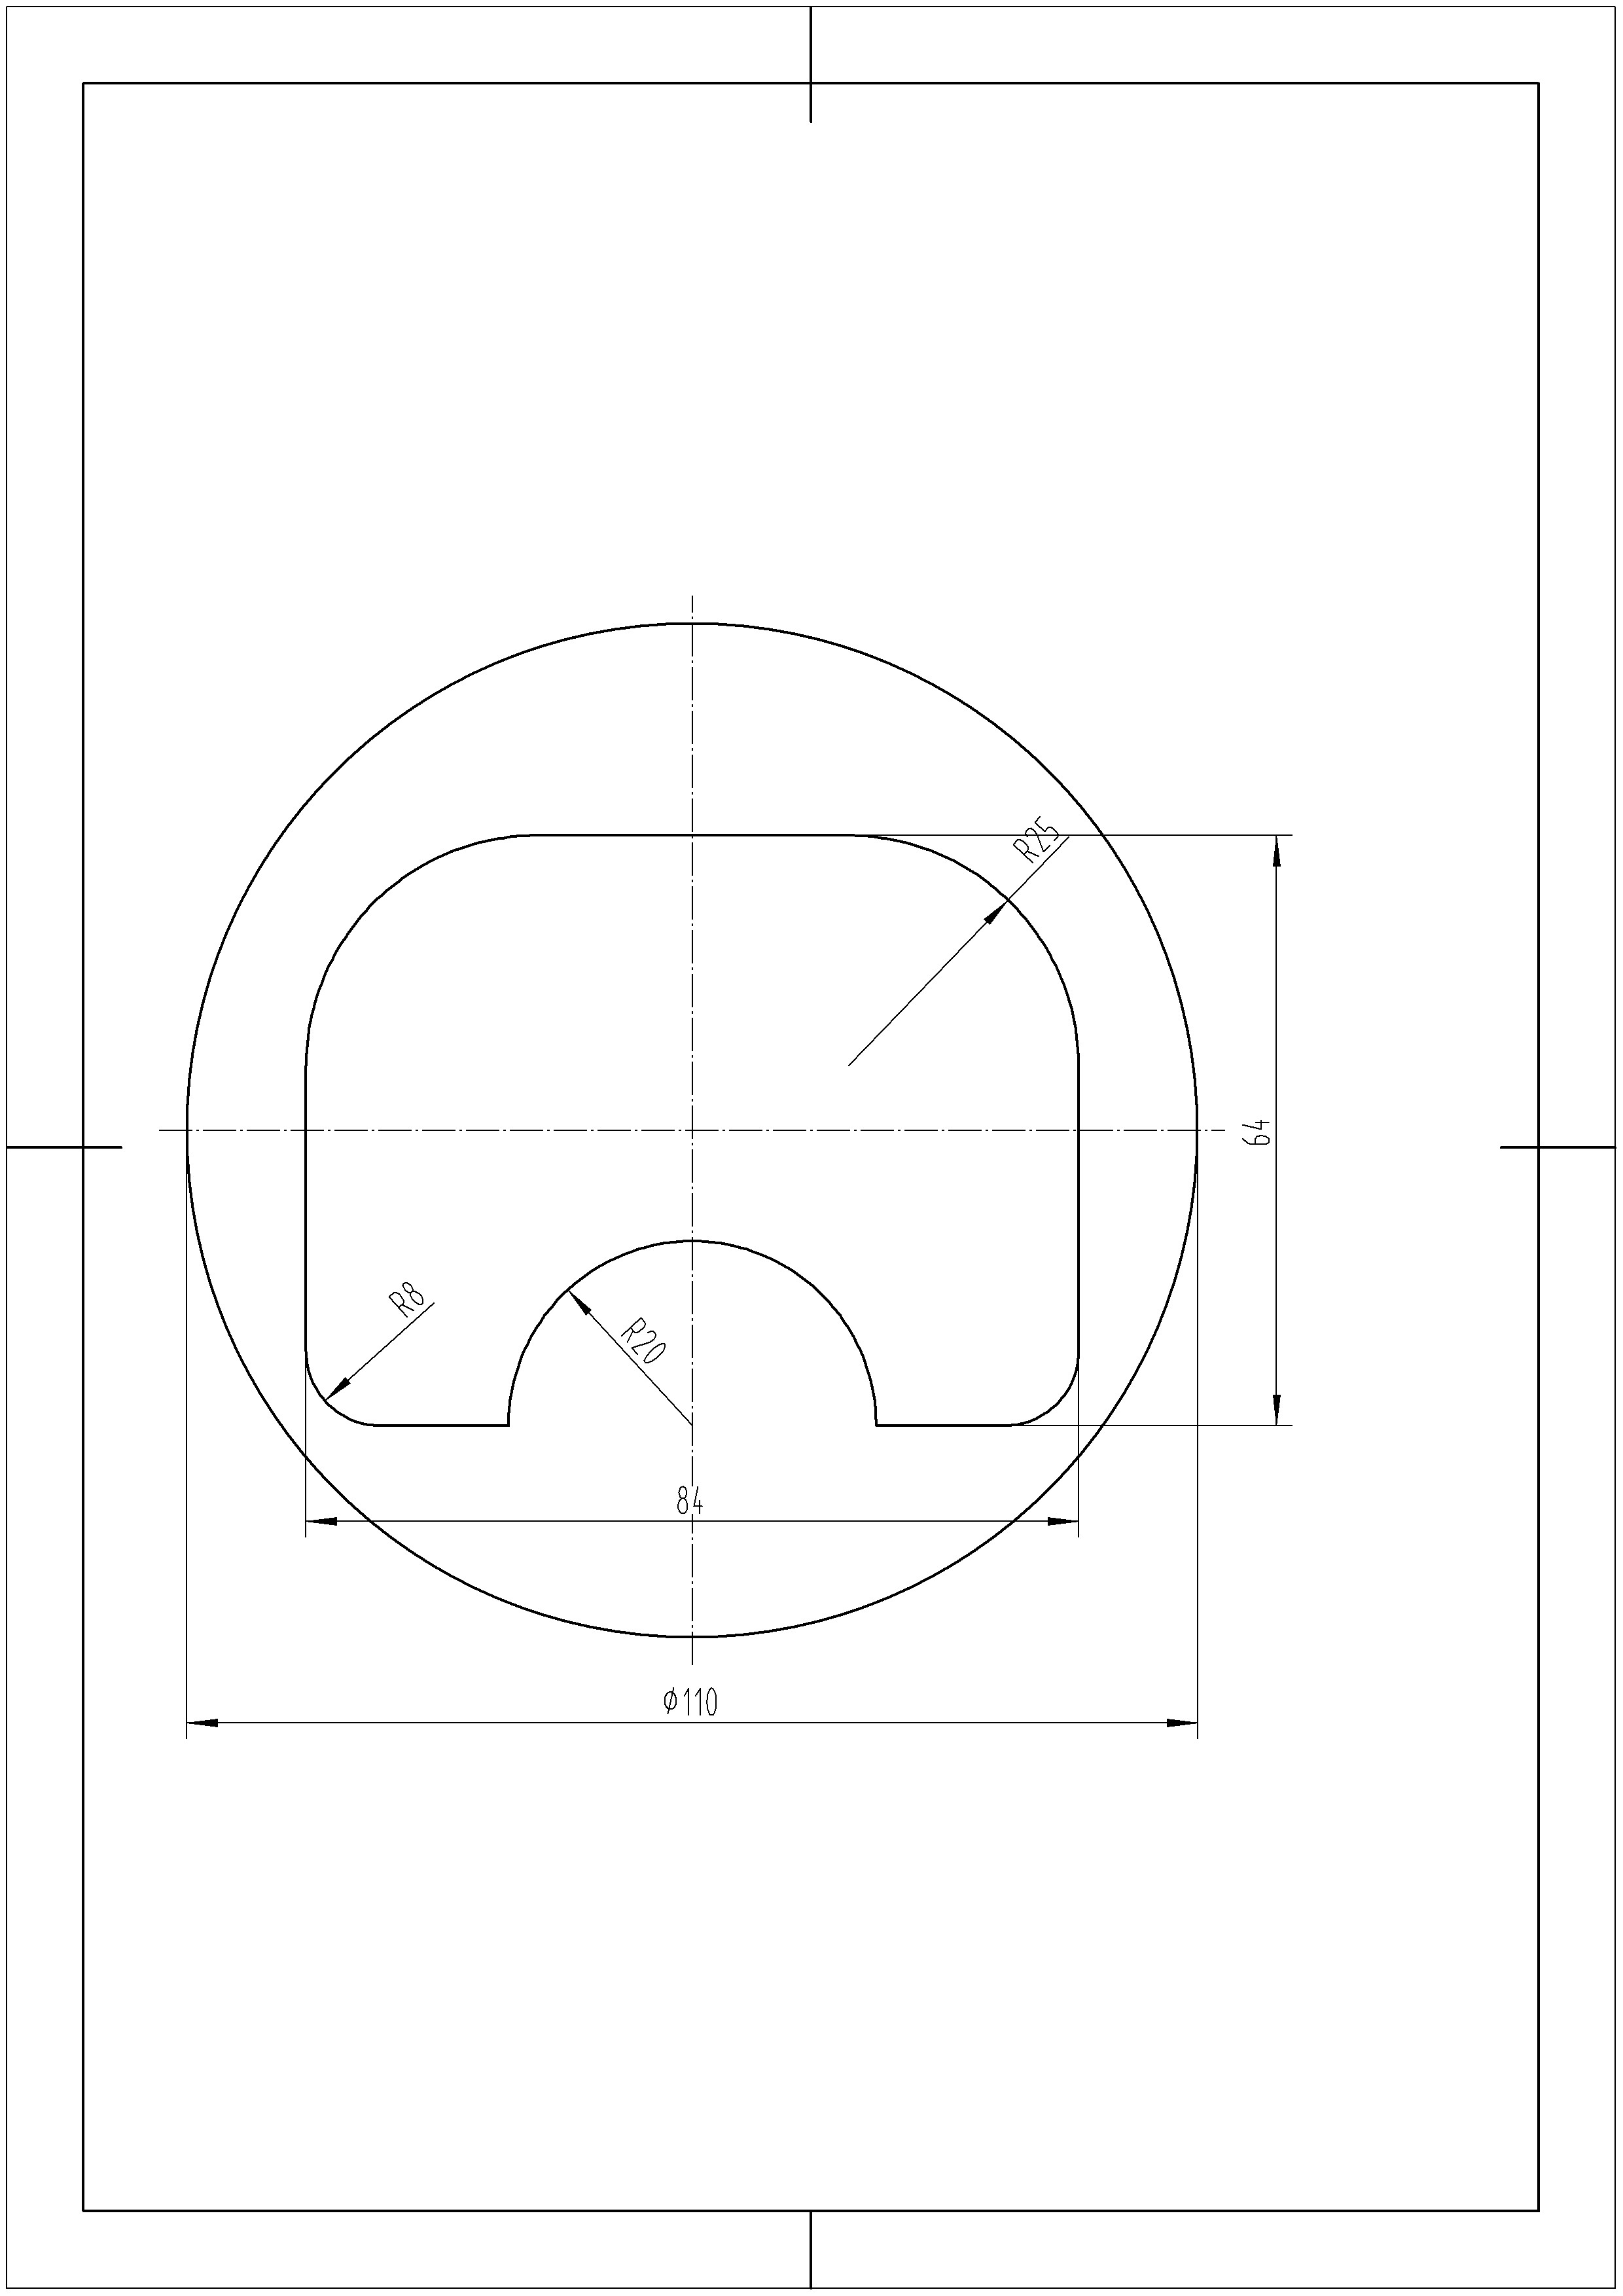
\includegraphics[width=0.8\linewidth,trim=40 150 70 220,clip]{data/image/7-2.jpg}
	\caption{复习实例2}
	\label{fig:8-1}
\end{figure}
\end{enumerate}


\subsection{教学内容及过程}

\subsubsection{刀具半径补偿}

由CNC系统内部使刀具在加工时,自动偏移一个刀具半径。
简化编程的难度。

指令G40、G41/G42

1、补偿方向的确定:

ISO 标准规定,当刀具中心轨迹在编程轨迹前进方向的左边时,称为左刀补,用G41表示;刀具中心轨迹在编程轨迹前进方向的右边时,称为右刀补,用G42表示;注销刀具半径补偿时用G40表示。

\begin{figure}[h]
	\centering
	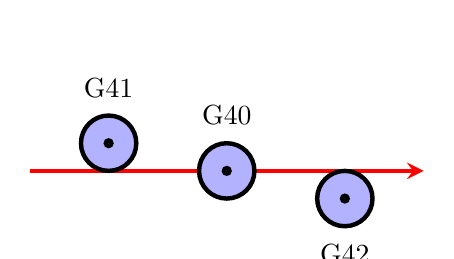
\begin{tikzpicture}[ultra thick]
	\draw[->,red,>=stealth]  (0,0) -- (5,0);
	\draw[fill=blue!30] (1,10pt) circle (10pt) circle (1pt);
	\draw[fill=blue!30] (2.5,0) circle (10pt) circle (1pt);
	\draw[fill=blue!30] (4,-10pt) circle (10pt) circle (1pt);
	\node at (1,30pt) {G41};
	\node at (2.5,20pt) {G40};
	\node at (4,-30pt) {G42};
	\end{tikzpicture}
	\caption{刀补位置}
	\label{fig:7-1}
\end{figure}

2、补偿值的设定:

通过参数进行设定:

[OfFset]---[补偿]----[位置号]----[D形状+D磨shen损]

3、指令的格式:

在开始刀补的位置,结合G1指令设定补偿方向及补偿值位置号,在结束的位置,用G40结合G1指令即可:

G41/G42 G1 X\_ Y\_  D\_;

……

G40 G1 X\_ Y\_;

4、补偿平面

可以在G18及G19平面上进行刀具半径补偿,(常用于球头刀)

5、补偿过程分析:

1)刀具半径补偿建立:当输入BS缓冲器的程序段包含有G41/G42命令时,系统认为此时已进入刀补建立状态。当以下条件成立时,加工中心以移动坐标轴的形式开始补偿动作。 

a. 有G41或G42被指定; 

b. 在补偿平面内有轴的移动; 

c. 指定了一个补偿号或已经指定一个补偿号但不能是D00;

d. 偏置(补偿)平面被指定或已经被指定; 

e. G00或G01模式有效。 

2) 补偿模式:在刀具补偿进行期间,刀具中心轨迹始终偏离编程轨迹一个刀具半径值的距离。此时半径补偿在G00、G01、G02、G03情况下均有效。 

3) 取消补偿:使用G40指令消去程序段偏置值,使刀具撤离工件,回到起始位置,从而使刀具中心与偏程轨迹重合。当以下两种情况之一发生时加工中心补偿模式被取消。

①给出G40同时要有补偿平面内坐标轴移动。

②刀具补偿号为D00。

4)不同平面内的半径补偿 

刀具半径补偿用G17、G18、G19命令在被选择的工作平面内进行补偿。即当G18命令执行后,刀具半径补偿仅影响X、Z移动,而对Y轴没有作用。


\subsubsection{注意事项}
1、G41/G42必须与G1/G0结合使用,不可在G2/G3圆弧指令下使用。

2、刀具必须在加工平面内有移动。

3、使用与取消必须成对使用。

4、加工前必须设定其补偿值。

5、切入前指定、切出后取消。

\subsubsection{加工实例}
毛坯:φ110*35

刀具:φ12立铣刀

加工路径:如图\ref{fig:8-2}所示:

\begin{figure}[h]
	\centering
	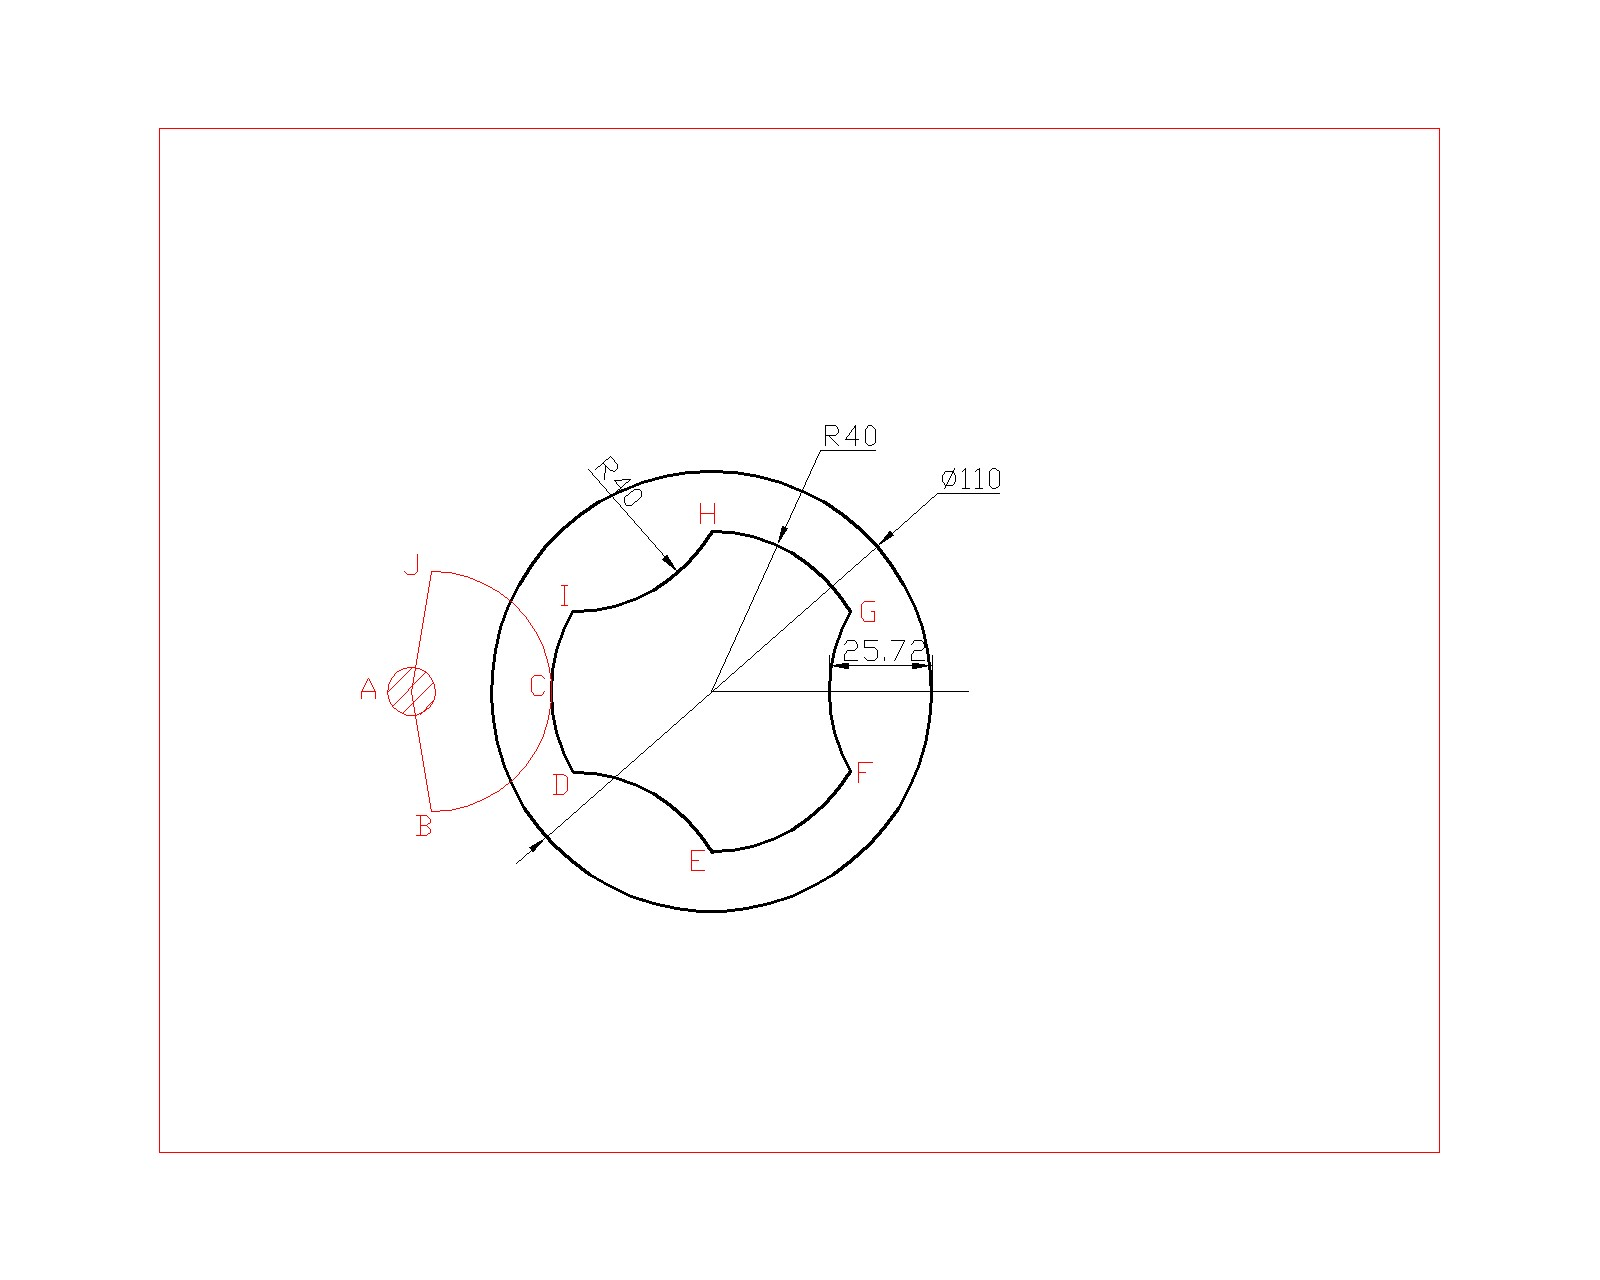
\includegraphics[width=0.8\linewidth,trim=280 250 430 280,clip]{data/image/8-2.jpg}
	\caption{刀补实例}
	\label{fig:8-2}
\end{figure}

参考程序:
\begin{lstlisting}
G54G17G40G49G90
M03 S300
G0 X-70.0 Y0
Z5.0
G01 Z-5.0 F500
G41 G01 X-60 Y-20 D01
G03 X-40.0 Y0 R20.0
G02 X-34.641 Y20.0 R40.0
G03 X0 Y40.0 R40.0
G02 X34.641 Y20 R40.0
G03 Y-20.0 R40.0
G02 X0 Y-40.0 R40.0
G03 X-34.641 Y-20 R40.0
G02 X-40 Y0 R40.0
G03 X-60 Y0 R20.0
G40 G01 X-70 Y0
G0 Z30
M05
M30
\end{lstlisting}

\subsubsection{刀具半径补偿值的确定}

1、粗加工:

为半精/精加留余量:0.2-0.6 (单边)

Offset=D/2+余量

2、半精加工:

为精加留余量:0.1-0.2 (单边)

Offset=D/2+余量

3、精加工:

Offset= Offset (上次)+修正

修正=(理论值-测量值)双边/2 

4、处多余材料:

Offset值不能太大



\subsection{课堂小结}
\begin{enumerate}[1、]
\item 刀补的概念
\item G40、G41/G42指令的使用;
\item 注意事项;
\item 刀补的编程;
\item 刀补值的计算。
\end{enumerate}

\vfill
\subsection{布置作业}
\begin{enumerate}[1、]
	\item 写出上面的程序。
\item 习题集。
\end{enumerate}
\vfill
\jxhj{%教学后记
	}
\skrq{%授课日期
	2017年10月12日 4-5节}
\ktmq{%课题名称
	 刀具半径补偿的应用(二)}
\jxmb{%教学目标,每行前面要加 \item
	\item 掌握Fanuc上极坐标指令的使用;
	\item 掌握Siemens上极坐标指令的使用;
	\item 灵活使用极坐标指令进行编程;
	\item 掌握加工工艺的分析。 }
\jxzd{%教学重点,每行前面要加 \item
	\item 极坐标知识和其指令的使用;
	\item 对加工轮廓进行处理后再编程。 }
\jxnd{%教学难点,每行前面要加 \item
	\item 加工轮廓进行处理后再编程。 }
\jjff{%教学方法
	通过讲述、举例、演示法来说明;}

\makeshouye %制作教案首页

%%%%教学内容
\subsection{组织教学}
\begin{enumerate}[\hspace{2em}1、]
	\item 集中学生注意力;
	\item 清查学生人数;
	\item 维持课堂纪律;
\end{enumerate}
\subsection{复习导入及主要内容}
\begin{enumerate}[1、]
	\item 旋转可应用场合;
	\item 要素及原理;
	\item Fanuc旋转指令格式;
	\item Sienes旋转指令格式;
	\item 编程实例。
\end{enumerate}



\subsection{教学内容及过程}

\subsubsection{加工轮廓的处理}
\begin{figure}[!hbtp]
	\centering	\includegraphics[width=0.8\textwidth]{images/9-1}
	\caption{极坐标实例} \label{极坐标实例}
\end{figure}
\textbf{加工轮廓的处理(改路径,延长)}
\paragraph{把加工轮廓进行拆分}
\noindent A、两个直槽:\\
标点的坐标,直角坐标(开放的)\\
B、小圆弧槽:\\
标点的坐标,使用极坐标\\
C、腰形槽:\\
标点的坐标,极坐标\\
D、扇形台阶\\
标点的坐标,极坐标\\
起点与终点不重合\\
编程时的处理\\
E、带翅膀的圆弧槽。
\paragraph{极坐标与 直角坐标的互换}
$$X=P*cosA$$
$$Y=P*sinA$$
$$P=X2+Y2$$
$$A=aictanY/X$$
\subsubsection{极坐标}
\paragraph{Fanuc上的极坐标}
指令格式: G\_\_ G~~ G16;启动极坐标指令(极坐标方式)\\
G~~ IP\_\_; 极坐标指令\\
:\\
G15;取消极坐标\\
说明:G\_\_极坐标指令的平面选择(G17、G18、G19)\\
G~~ G90指定工件坐标系的零点作为极坐标系原点,\\
G91指定当前位置作为极坐标系的原点。\\
IP\_\_指定极坐标系选择平面的轴地址及其值。\\
第1轴:极坐标半径\\
第2轴:极坐标角度 \\
用G90指定半径,极点设在工件坐标系原点。\\
如再用G90指定角度,角度是与X轴的夹角\\
如再用G91指定角度,角度是与当前位置的夹角\\
用G91指定半径,极点设在刀具当前位置。\\
如再用G90指定角度,角度是与X轴的夹角\\
如再用G91指定角度,角度是与当前位置的夹角。\\
限制:A、在极坐标方式中,对圆弧插补或螺旋线插补(G02,G03)用R 指定半径。\\
在极坐标方式中,不能用以下指令:\\
G4、G10、G52、G92、G53、G68、G51\\
在极坐标方式中不能倒角和倒圆\\
\paragraph{Siemens上的极坐标}
\textbf{极坐标,极点定义}:G110,G111,G112 \\
A、在直角坐标系中定义极点:\\
G110/G111/G112 X\_\_ Y\_\_ Z\_\_\\
B、在极坐标系中定义极点:\\
G110/G111/G112 AP=\_\_RP=\_\_\\
说明: \\
G110:相对于刀具最近到达的点(刀具当前位置)定义极点\\
G111:相对于当前工件坐标系定义极点\\
G112:相对于上一个有效极点定义极点\\
\textbf{在极坐标系中使用极坐标}\\
A、G0 AP=\_\_ RP=\_\_\\
B、G1 AP=\_\_ RP=\_\_\\
C、G2 AP=\_\_RP=\_\_\\
D、G3 AP=\_\_ RP=\_\_
说明:\\
AP=\_\_:极角,极点和目标点之间连线与角度参考方向之间的夹角(第一次角度参考方向线中一条),取值范围±(0-360),当用绝对坐标编程时,角度为相对于加工平面的水平轴方向,当用相对坐标编程时,上一个被编程角度作为参考位置。极角一直保持到新的极角被定义或工件坐标系被改变。\\
RP=\_\_:极半径,极点和目标点之间的距离,极半径一保持到新的极半径被定义。\\
所有与极坐标有关的输入必须在单个程序段内编程。用极坐标所定义的位置都可以用G0 G1 G2 G3去移动,极坐系在由G17/G18/G19所定义的加工平面内都有效。如果没有极坐标在使用,有效的工件坐标系的原点有用,\\
\subsubsection{加工工序} \marginpar{ 比较分析讲解}
A、铣上表面\\
B、铣ф30通孔(也可钻、扩、镗)\\
C、铣直槽和圆弧\\
……
由学生自己分析。\\


















\subsection{课堂小结}
\begin{enumerate}[1、]
	\item 加工轮廓的处理;
	\item 极坐标;
	\item 加工工序。
\end{enumerate}

\vfill
\subsection{布置作业}
\begin{enumerate}[1、]
	\item 自选一零件图, 写出其工艺与程序。 
\end{enumerate}
\vfill
\jxhj{%教学后记
	}
\skrq{%授课日期
	2017年10月17日 4-5节}
\ktmq{%课题名称
	 子程序概述及Z向分层}
\jxmb{%教学目标,每行前面要加 \item
	\item 掌握子程序的概念;
	\item 掌握子程序命令的使用;
	\item 掌握使用子程序进行Z向分层的思路;
	\item 掌握掌握子程序的编程。 }
\jxzd{%教学重点,每行前面要加 \item
	\item Z向分层的思路;
	\item 子程序命令的使用。 }
\jxnd{%教学难点,每行前面要加 \item
	\item Z向分层的思路。 }
\jjff{%教学方法
	通过讲述、举例、演示法来说明;}

\makeshouye %制作教案首页

%%%%教学内容
\subsection{组织教学}
\begin{enumerate}[\hspace{2em}1、]
	\item 集中学生注意力;
	\item 清查学生人数;
	\item 维持课堂纪律;
\end{enumerate}
\subsection{复习导入及主要内容}
\begin{enumerate}[1、]
	\item 用刀补去残料的思路。
\item 去材料刀补的计算;
\item 多个刀补的编程;
\item 巩固粗/精加工刀补值的确定。
\end{enumerate}

\subsection{教学内容及过程}

\subsubsection{Fanuc上子程序的格式及调用}
[ 格式 ]
■子程序构成

O55; 子程序名

G1 ...

.

.

.

M99;子程序结束


■	子程序呼叫

M98P55L1

[ 说明 ]

当主程序呼叫子程序时,它是一重子程序呼叫。因此,子程序可以做四重呼叫,。                                                 

一个单个呼叫指令可以重复呼叫子程序最多到9999次。

对于兼容的编程装置,在第一个单节里,Nxxxx可以代替子程序O(或:)跟着的数字。在N后面的顺序号被认为是子程序号。

[ 注意 ]
1.	M98和M99信号不输出到机床。
2.	不到位址指定的子程序号,输出报警(No. 078)。

[ 举例 ]

☆M98 P51002;

这条指令指定“呼叫子程序(程序号1002)5次”。

子程序呼叫指令(M98P\_\_\_)可以在移动指令单节中指定。

☆X1000.0 M98 P1200;

这个例子在X轴移动之后呼叫子程序(子程序号 1200)。

☆从主程序呼叫子程序的执行顺序

主程序                   子程序

N0010 O;               N0010 O;   
      
N0020 O;               N0020 O;    
     
N0030 M98 P21010;      N0030 M98 P21010; 
                
N0040 O;               N0040 O;
             
N0050 O;               N0050 O;

子程序可以象主程序呼叫子程序一样呼叫另一个子程序。

[ 特殊用途 ]
 
■主程序中使用M99

如果在主程序中执行M99,控制返回主程序开头。

举例说,/M99放在程序中并执行M99;

在主程序的适当位置设定选择性单节跳跃功能,在执行主程序时关掉。

当执行M99时,控制返回到主程序的开头,然后主程序从头开始重复执行。

当选择性单节跳跃功能设定关时,重复执行程序。当选择性单节跳跃功能设定开时,/M99单节被跳过;控制进入下一个单节继续执行。

二、使用子程序的场合:

1、同一零件上有重复加工的部位

2、批量加工,一次加工多个相同的工件

3、同一个零件上有多个不同形状的加工轮廓

可使程序看起来方便,简单

不使用的场合:

自动编程不用子程序:


1、多程序传输不方便

2、自动编程子程序完成后,修改的内容多,

三、编程实例

方形:

\begin{lstlisting}
O0001
G54G17G40G49G90
M3S500
G1Z30.F2000
X-50.Y0
Z5.0
Z0F200
D1M98P40002
G1Z30.F2000
M4
M30
O0002
G91G1Z-5.0
G90G41X-40.Y0
G3X-30.Y0R10.
G1Y30.
….
M99
\end{lstlisting}

\subsection{课堂小结}
\begin{enumerate}[1、]
	\item 加工轮廓的处理;
	\item 极坐标;
	\item 加工工序。
\end{enumerate}

\vfill
\subsection{布置作业}
\begin{enumerate}[1、]
	\item 自选一零件图, 写出其工艺与程序。 
\end{enumerate}
\vfill
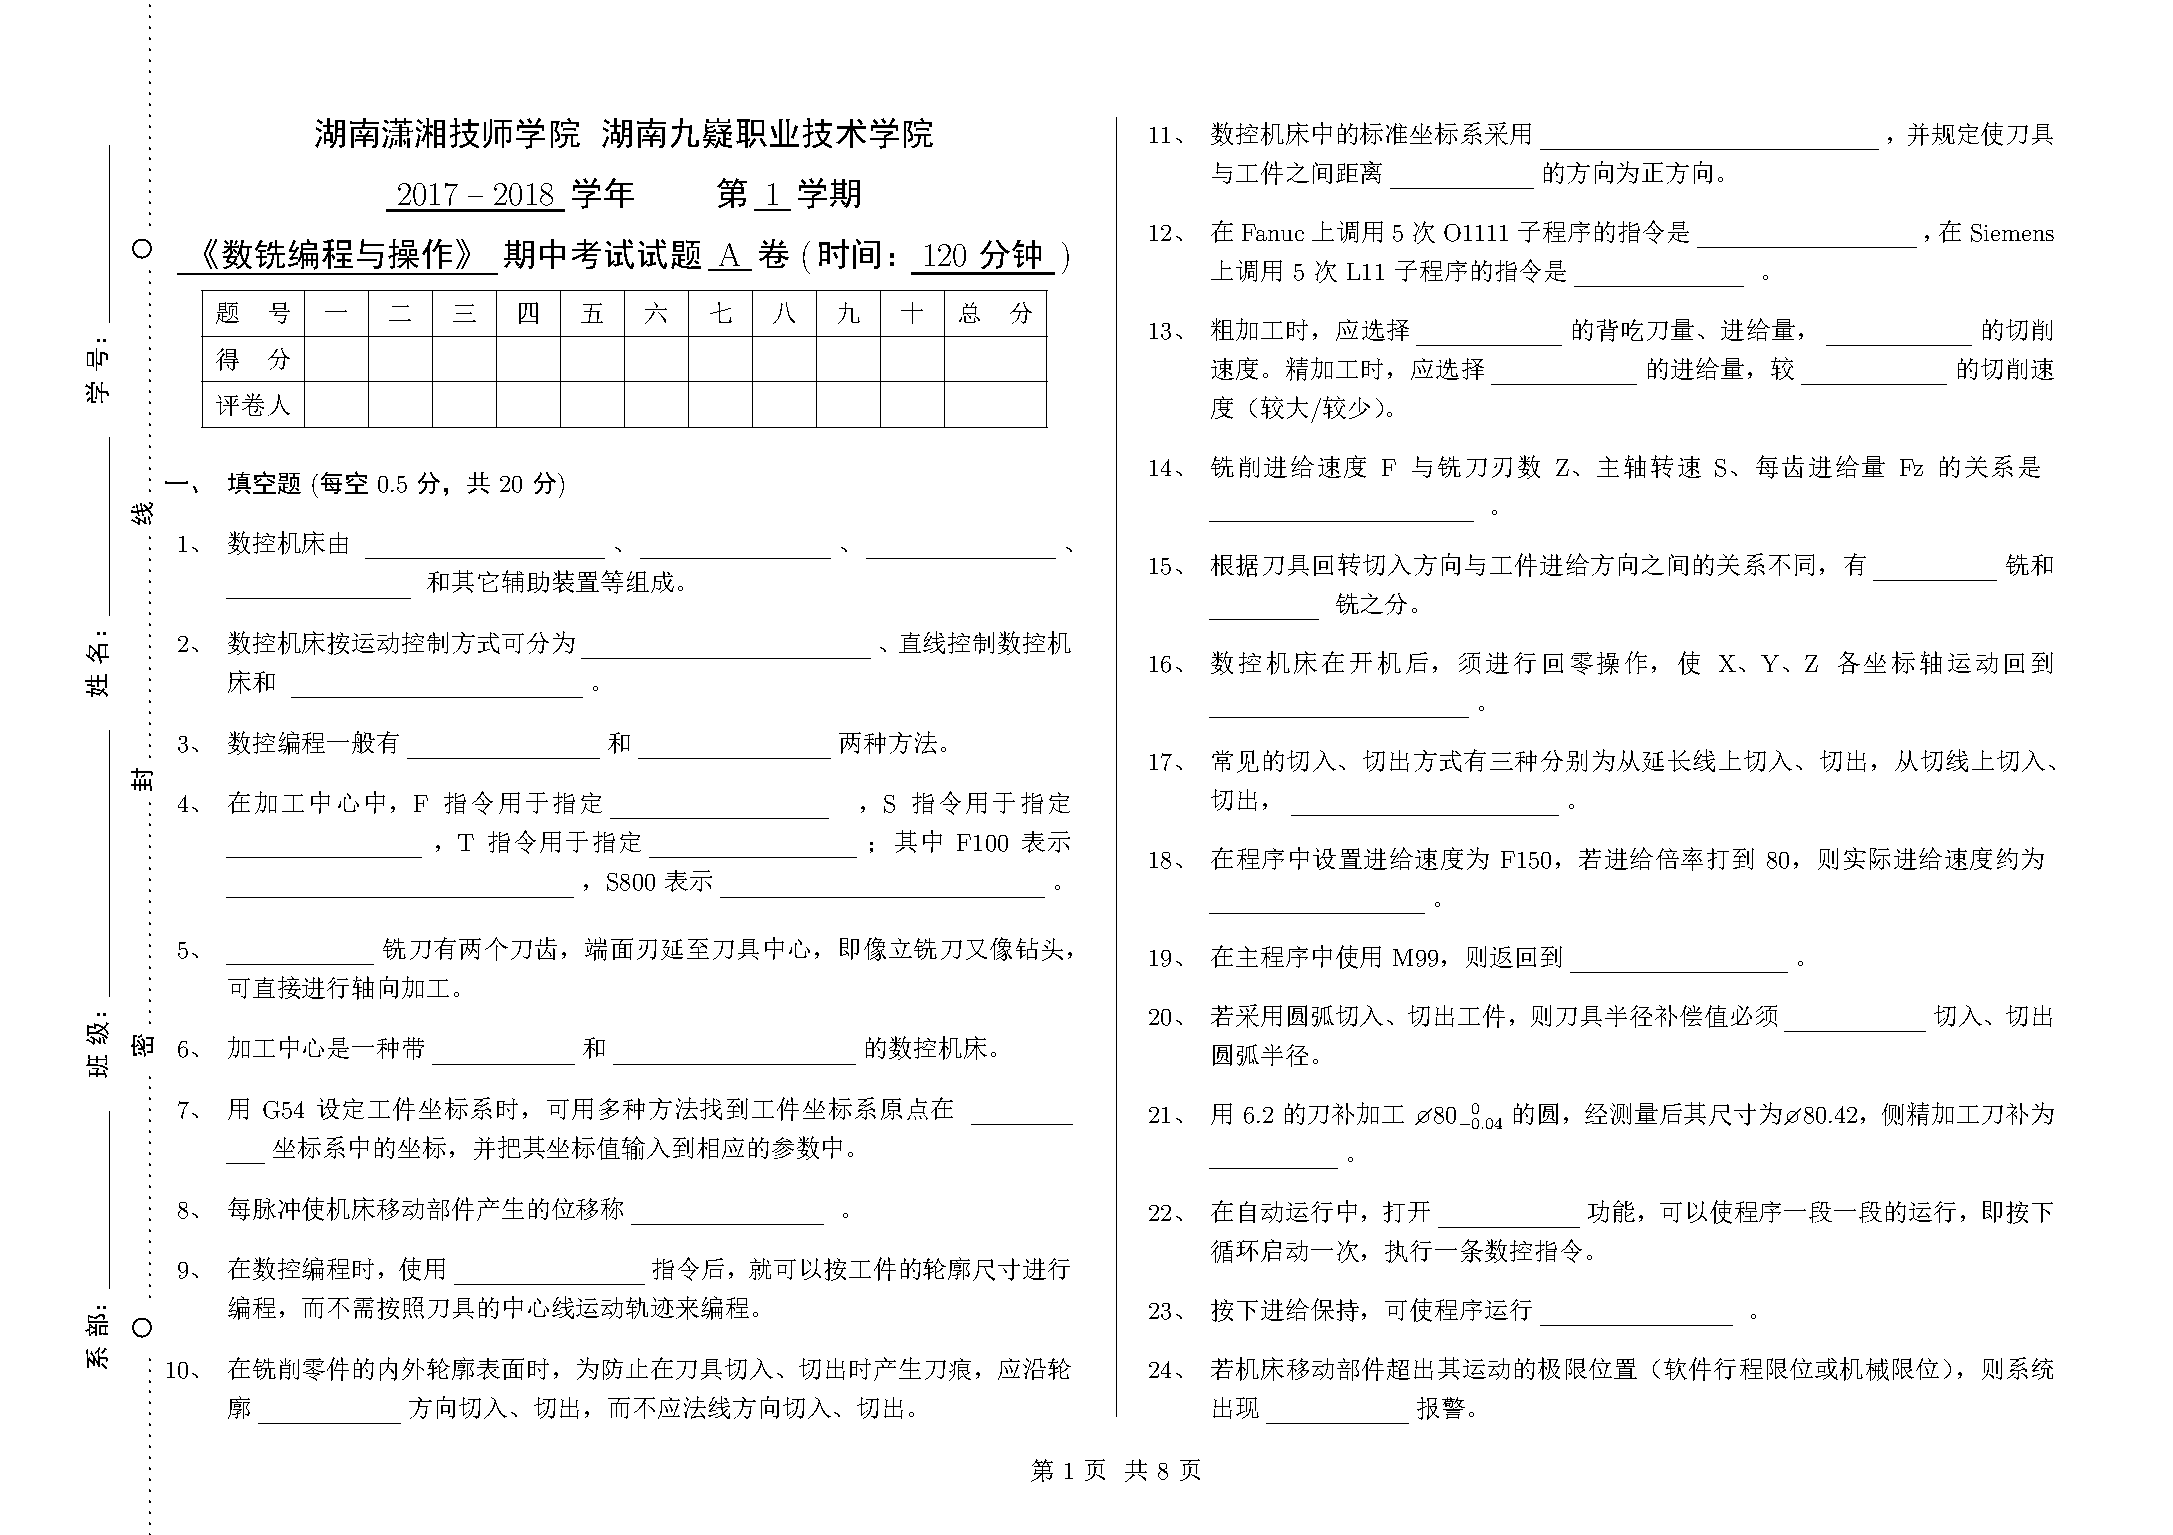
\includepdf[pages={-},landscape=true]{shijuan.pdf}
%\jxhj{%教学后记
	}
\skrq{%授课日期
	2017年10月19日 4-5节}
\ktmq{%课题名称
	 子程序的XY向分层}
\jxmb{%教学目标,每行前面要加 \item
	\item 掌握子程序指令的使用;
	\item 掌握用子程序编程;
	\item 掌握用子程序及刀补实现XY向分层;
	\item 掌握子程序的嵌套调用。 }	
\jxzd{%教学重点,每行前面要加 \item
	\item 用子程序及刀补实现XY向分层;
	\item 子程序的嵌套调用。 }
\jxnd{%教学难点,每行前面要加 \item
	\item 用子程序及刀补实现XY向分层。 }
\jjff{%教学方法
	通过讲述、举例、演示法来说明;}

\makeshouye %制作教案首页

%%%%教学内容
\subsection{组织教学}
\begin{enumerate}[\hspace{2em}1、]
	\item 集中学生注意力;
	\item 清查学生人数;
	\item 维持课堂纪律;
\end{enumerate}
\subsection{复习导入及主要内容}
\begin{enumerate}[1、]
	\item 子程序的概念;
\item 子程序的组成;
\item 子程序的调用;
\item 子程序的使用。
\end{enumerate}


\subsection{教学内容及过程}

\subsubsection{加工实例分析}

如图\ref{fig:11-1}所示:加工凸台零件,高12mm。

\begin{figure}[h]
	\centering
	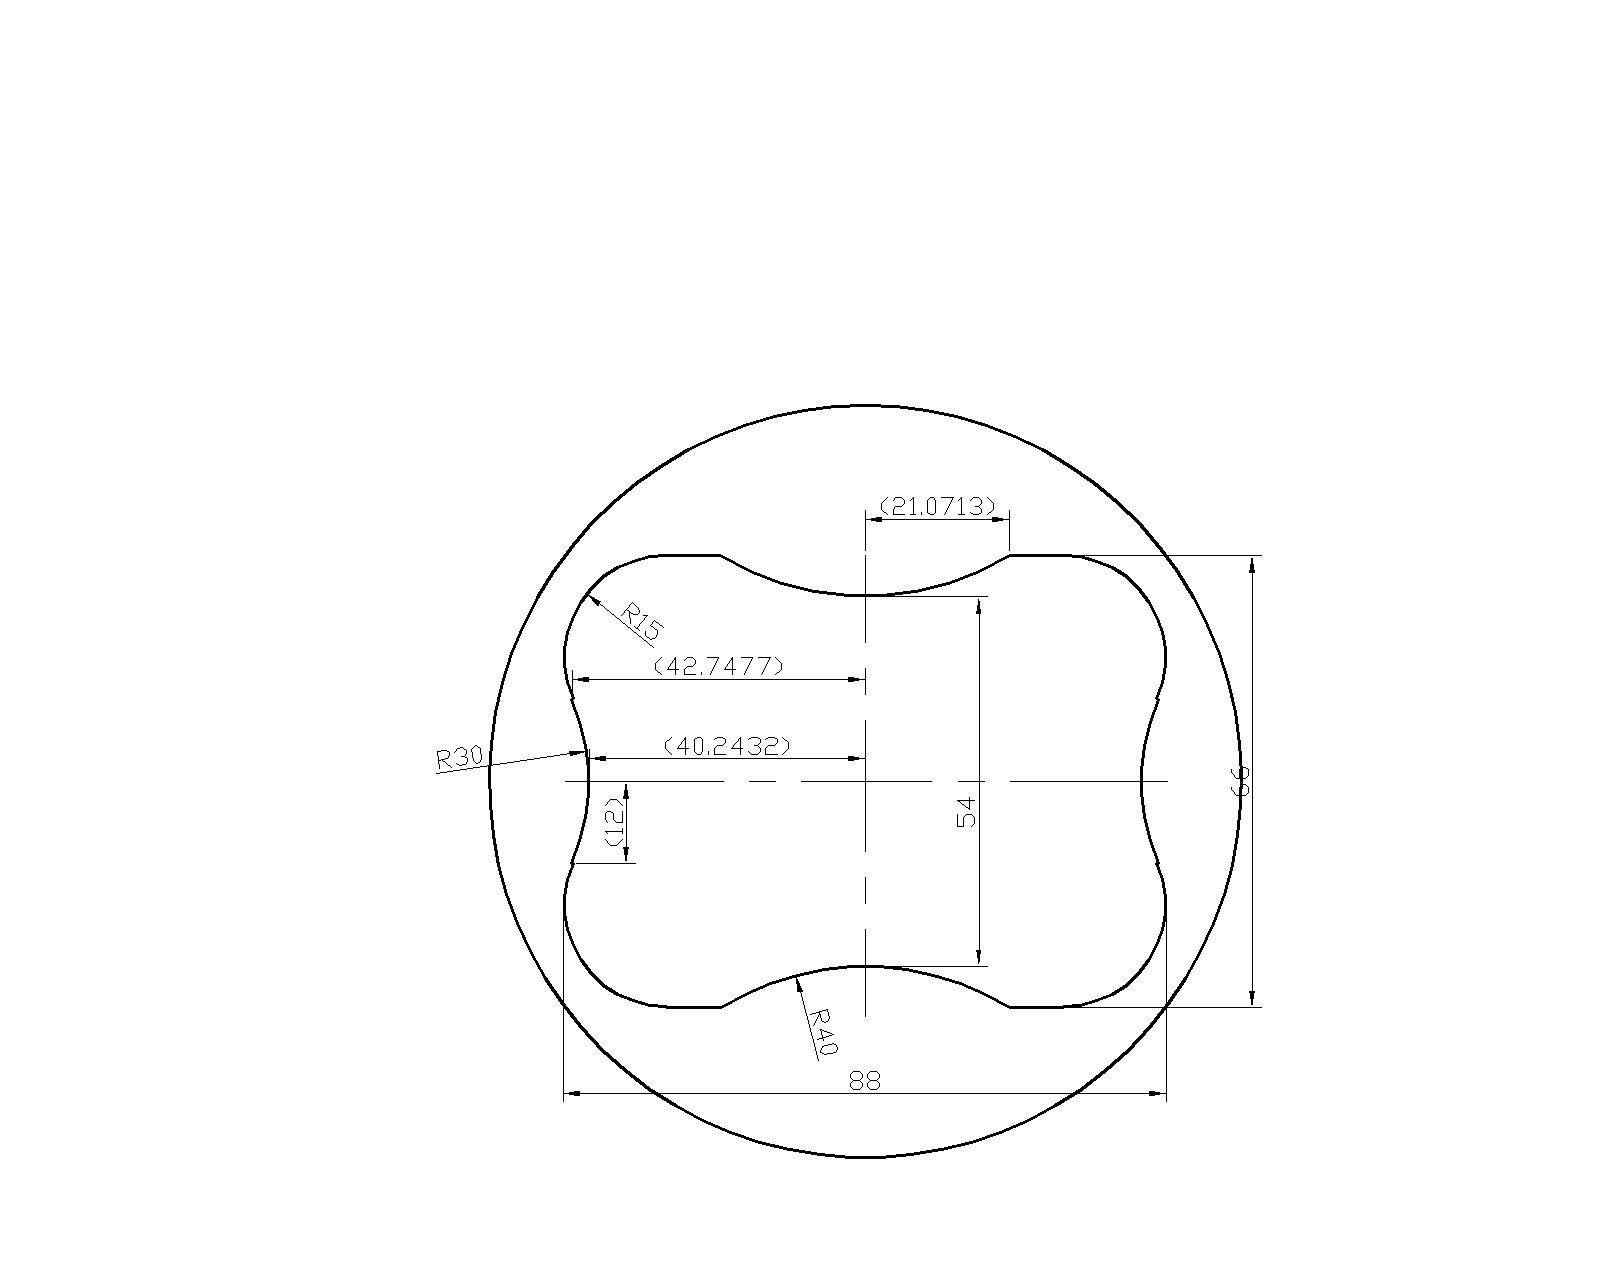
\includegraphics[width=0.7\linewidth,trim=250 50 150  250,clip]{data/image/11-1.jpg}
	\caption{刀补实例}
	\label{fig:11-1}
\end{figure}

毛坯:\diameter 110*35

刀具:\diameter 12立铣刀

1、Z向分层加工:

高12mm     3mm*4次     深度等分下刀

用G91 G01 Z-3.0 F300; Z方向要先定好位

是Z方向

2、XY向分层,平面上的等分铣削:

方法:用不同的刀具半径值:

A、刀具补偿值的确定:(由小到大确定)

大=较大+B

较大=小+B

小=D/2+(0.2-0.6)

B=50-80\% *D 

判断是否把多余材料去完

B、切入/切出圆弧半径:

R>最大的刀补值

C、XY平面内的定位

第一次铣削后,刀具位置应回到原来位置

3、参考程序:

主程序:


\begin{lstlisting}
O0001
G54 G17 G40 G49 G90
M03 S300
G01 X0 Y75.0 F800
Z0
M98 P40002
G01 Z30.0
M05
M30
\end{lstlisting}

下刀子程序
\begin{lstlisting}
O0002
G91 G01 Z-3.0 
G90
D1 M98 P3
D2 M98 P3
D3 M98 P4
M99
\end{lstlisting}
轮廓子程序
\begin{lstlisting}
O0003
G41 G01 X-40.0 Y67.0
G03 X21.071 Y33.0 R40.0
G1 X39
G03 X42.748 Y12.0 R15.0
G02 Y-12.0 R30.0
G03 X39 Y-33.0 R15.0
G01 X21.071
G03 X-21.071 R40.0
G01 X-39.0
G03 X-42.748 Y-12.0 R15.0
G02 Y12.0 R30.0
G03 X-39.0 Y33.0 R15.0
G01 X-21.071 
G03 X40.0 Y67.0 R40.0
G40 G01 X0 Y75.0
M99
\end{lstlisting}

\subsubsection{使用子程序的场合}
1、同一零件上有重复加工的部位

2、批量加工,一次加工多个相同的工件

3、同一个零件上有多个不同形状的加工轮廓

可使程序看起来方便,简单

不使用的场合:

自动编程不用子程序:

1、多程序传输不方便

2、自动编程子程序完成后,修改的内容多。

\subsection{课堂小结}
\begin{enumerate}[1、]
	\item 子程序Z向分层;
	\item 子程序XY向分层;
	\item 子程序的应用。	
\end{enumerate}

\vfill
\subsection{布置作业}
\begin{enumerate}[1、]
	\item 用子程序编写一个Z向分层+XY向分层的程序。 
\end{enumerate}
\vfill
%\jxhj{%教学后记
	}
\skrq{%授课日期
	2017年10月24日 4-5节}
\ktmq{%课题名称
	 siemens编程应用}
\jxmb{%教学目标,每行前面要加 \item
	\item 掌握孔系的宏程序加工方法;
	\item 掌握孔系的编程思路;
	\item 掌握循环嵌套的使用;
	\item 分清Fanuc与Siemens的指令格式。 }
\jxzd{%教学重点,每行前面要加 \item
	\item 孔系的宏程序;
	\item 孔系的编程思路。 }
\jxnd{%教学难点,每行前面要加 \item
	\item 孔系的编程思路。 }
\jjff{%教学方法
	通过讲述、举例、演示法来说明;}

\makeshouye %制作教案首页

%%%%教学内容
\subsection{组织教学}
\begin{enumerate}[\hspace{2em}1、]
	\item 集中学生注意力;
	\item 清查学生人数;
	\item 维持课堂纪律;
\end{enumerate}
\subsection{复习导入及主要内容}
\begin{enumerate}[1、]
	\item 加工轮廓的处理;
	\item 极坐标;
	\item 加工工序。
\end{enumerate}


\subsection{教学内容及过程}


\subsubsection{在Fanuc上用G91+K来实现孔系加工}

\begin{lstlisting}[language=C]
O0001
G54G17G40G49G90
M3S500
G1Z30.F2000
X0Y0
G99G81X20.Y20.Z-20.R5.F80 K6
G1Z30.F2000
M5
M30
\end{lstlisting}

\subsubsection{宏程序来实现}

\begin{lstlisting}[language=C]
#24=  圆周圆心的X坐标绝对值
#25=  圆周圆心的Y坐标绝对值 
#26=  孔深Z坐标绝对值 
#18=  快速趋近点R坐标
#9=   切削进给速度F
#4=   圆半径1
#1=   第一孔的角度
#2=   增量角B
#11=  孔数H
G54G17G40G49G90
M3S800
G52 X#24 Y#25
G1 Z30.F2000
#8=1
WHILE[#8LE#11] DO1
#5=#4*COS[#1+[#8-1]*#2]
#5=#4*SIN[#1+[#8-1]*#2]
G99G81X#5Y#6Z#26R#18F#9
#8=#8+1
END1;
G1Z30.F2000
G52 X0 Y0
M5
M30
\end{lstlisting}


\subsubsection{方形阵列孔加工}

\begin{lstlisting}[language=C]
#1= 矩阵孔群横向中心连线与X轴的夹角
#2= 矩阵孔群横向中心与纵向中心连线角度
#3= 矩阵横向孔中心距
#4= 矩阵纵向孔中心距
#5= 矩阵横向孔数
#6= 矩阵纵向孔数
#9= 切削进给速度 Feed
#18= 固定循环中快速走近R点Z坐标
#24= 圆心X坐标
#25= 圆心Y坐标
#26= 孔深
G54G17G40G49G90
M3S500
G1Z30.F2000
G52 X#24 Y#25
G68 X0 Y0 R#1
#10=1
WHILE[#10LE#6]DO1
#11=1 
WHILE[#11LE#6]DO2
IF [[#10AND1]EQ0] GOTO1
#12=#3*[#11-1]+#4*COS[#2]*[#10-1]
#13=#4*SIN[#2]*[#10-1]
GOTO5
N1 #12=#3*[#5-#11]+#4*COS[#2]*[#10-1]
#13=#4*SIN[#2]*[#10-1]
N5 G99 G81 X#12 Y#13 Z#26 r#18 F#9
#11=#11+1
END2
#10=#10+1
END1
G80G1Z30.F2000
G69
G52 X0 Y0
M5
M30
\end{lstlisting}

\subsubsection{圆形阵列孔加工}

\begin{lstlisting}[language=C]
O0001
#1=40
#2=45
#3=8
#4=10
#5=5
S1000M3
G54G90  G1 X0 Y0 Z30
G16
#6=1
WHILE[#6LE#3]DO1
#7=1
WHILE[#7LE#5]DO2
#8=#1/2+[#7-1]*#4
#9=[#6-1]*#2
G99G81 X#8 Y#9 Z-6 R1 F80
#7=#7+1
END2
#6=#6+1
END1
G80G1Z30.F2000
G15
M5
M30
\end{lstlisting}

\subsubsection{混合孔的加工}

略



\subsection{课堂小结}
\begin{enumerate}[1、]
	\item 在Fanuc上用G91+K来实现孔系加工;
	\item 宏程序来实现;
	\item 方形阵列孔加工;
	\item 圆形阵列孔加工;
	\item 混合孔的加工。
\end{enumerate}

\vfill
\subsection{布置作业}
\begin{enumerate}[1、]
	\item 写出上面的程序;
	\item 从习题集上选做一个。
\end{enumerate}
\vfill
%\jxhj{%教学后记
	}
\skrq{%授课日期
	2017年5月22日 4-5节}
\ktmq{%课题名称
	 变量周边倒圆角}
\jxmb{%教学目标,每行前面要加 \item
	\item 掌握简单零件的倒圆;
	\item 掌握相关数学处理;
	\item 掌握循环的几个特点;
	\item 掌握简单零件的倒角。 }
\jxzd{%教学重点,每行前面要加 \item
	\item 掌握简单零件的倒圆;
	\item 掌握简单零件的倒角。 }
\jxnd{%教学难点,每行前面要加 \item
	\item 相关数学处理。 }
\jjff{%教学方法
	通过讲述、举例、演示法来说明;}

\makeshouye %制作教案首页

%%%%教学内容
\subsection{组织教学}
\begin{enumerate}[\hspace{2em}1、]
	\item 集中学生注意力;
	\item 清查学生人数;
	\item 维持课堂纪律;
\end{enumerate}
\subsection{复习导入及主要内容}
\begin{enumerate}[1、]
	\item 加工轮廓的处理;
	\item 极坐标;
	\item 加工工序。
\end{enumerate}


\subsection{教学内容及过程}

\subsubsection{简单零件的倒角}
如图\ref{园锥}所示:
\begin{figure}[!hbtp]
	\centering	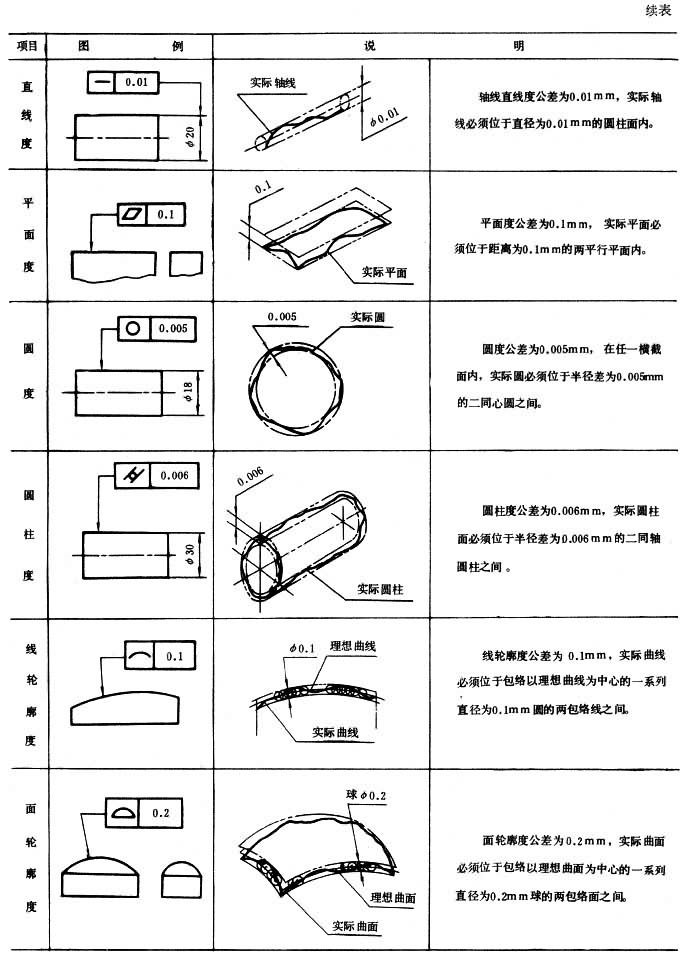
\includegraphics[width=0.4\textwidth]{images/13-1.jpg}
	\caption{圆锥} \label{圆锥}
\end{figure}
参考程序:
\begin{lstlisting}
O0001
#101=50
#102=20
#103=15
#104=8
#105=0.1
G54G17G40G49G90
M3S500
G1Z30.F2000
X-[#101/2+#104]Y0
Z5.0
Z-#102F200
#120=#102
WHILE[#120 GT 0]DO1
#120=#120-#105
G1Z-#120
#121=#101/2-[#102-#120]*TAN[#103]
X-[#121+#104] Y0
G2 I[#121+#104]
END1
G1 Z30.F2000
M5
M30
\end{lstlisting}
\subsubsection{写出如图\ref{圆角}所示零件的宏程序}
\begin{figure}[!hbtp]
	\centering	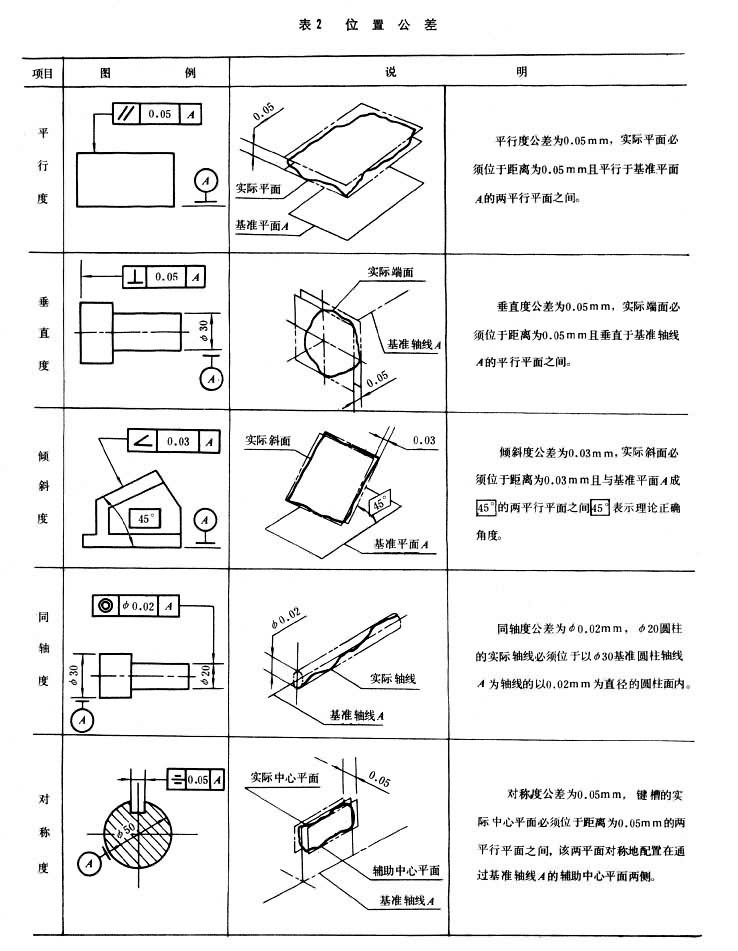
\includegraphics[width=0.4\textwidth]{images/13-2.jpg}
	\caption{圆角} \label{圆角}
\end{figure}
刀具半径: \#103

加工精度: \#104

Z向分层(用角度控制)

初始值: \#120=0

终止值: 90

\verb|#121=#102-#102*sin[#120]|

\verb|#122=#101/2-[#102-#102*cos[#120]]|

参考程序:
\begin{lstlisting}
O0001
#101----#104
G54G17G40G49G90
M3S500
G1Z30.F2000
X-[#101/2+#103+1]Y0
Z5.0
Z-#102F200
#120=0
WHILE[#120LT90]DO1
#120=#120+#104
#121=#102-#102*sin[#120]
G1Z-#121
#122=#101/2-[#102-#102*cos[#120]]
G1X-[#122+#103]Y0
G2I[#122+#103]
END1
G1Z30.F2000
M5
M30
\end{lstlisting}
\subsubsection{写出如图\ref{圆角:圆锥}所示零件的宏程序}:
\begin{figure}[!hbtp]
	\centering	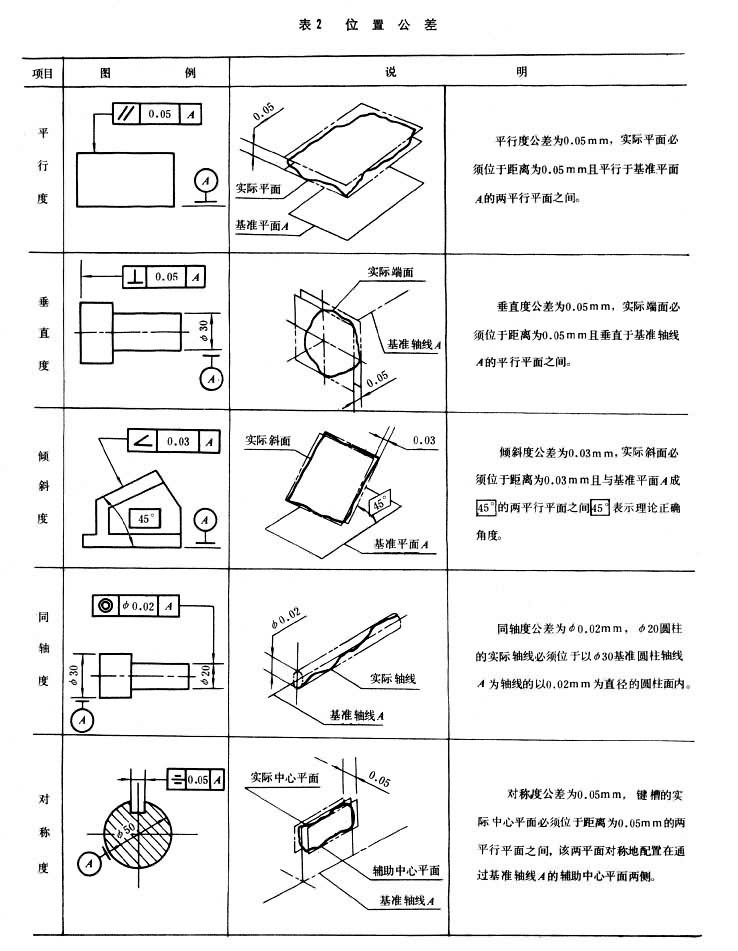
\includegraphics[width=0.4\textwidth]{images/13-2.jpg}
	\caption{圆角:圆锥} \label{圆角:圆锥}
\end{figure}
刀具:\#105

加工精度: \#106

角度精度: \#107

斜度:

Z向分层: 用长度控制

初始值: \#121=\#102

终止值为: \#102-\#131

\#131=\#102-\#103+\#103*SIN[\#104]

\#122=\#101-[\#102-\#121]*TAN[\#121]

圆角:

Z向分层:用角度控制

初始值: \#120=\#104

终止值: 90

\#121=\#103-\#103*sin[\#120]

\#122=\#132+\#103*cos[\#120]

\#132=\#103-\#131*tan[\#103]-\#102*cos[\#103]

参考程序:

\begin{lstlisting}
O0001
#101----#107
G54G17G40G49G90
M3S500
G1Z30.F2000
X-[#101+#105+2] Y0
Z5.0
Z-#102F200
#121=#102
#131=#102-#103+#103*SIN[#104]
WHILE[#121GT#131]DO1
#121=#121-#106
IF[#121LT#131]THEN#121=#131
G1Z-#121
#122=#101-[#102-#121]*TAN[#121]
X-[#122+#105]Y0
G2I[#122+#105]
END1
#132=#103-#131*tan[#103]-#102*cos[#103]
#120=#104
WHILE[#120LT90]DO1
#120=#120+#107
IF[#120GT90]THEN#120=90
#121=#103-#103*SIN[#120]
#122=#132+#103*COS[#120]
G1Z-#121
X-[#122+#105]Y0
G2I[#122+#105]
END1
G1Z30.F2000
M5
M30
\end{lstlisting}

\subsection{课堂小结}
\begin{enumerate}[1、]
	\item 简单零件的倒角;
	\item 宏程序实例1;
	\item 宏程序实例2。
\end{enumerate}

\vfill
\subsection{布置作业}
\begin{enumerate}[1、]
	\item 写出上面的程序;
	\item 从习题集上选做一个。
\end{enumerate}
\vfill
%\jxhj{%教学后记
	}
\skrq{%授课日期
	2017年10月31日 4-5节}
\ktmq{%课题名称
	 外轮廓加工}
\jxmb{%教学目标,每行前面要加 \item
	\item 掌握增加刀路去残料的思路;
	\item 掌握增加刀路的方法;
	\item 掌握相关点的计算;
	\item 会合理的增加刀路	。 }
\jxzd{%教学重点,每行前面要加 \item
	\item 增加刀路去残料的思路;
	\item 增加刀路的方法。 }
\jxnd{%教学难点,每行前面要加 \item
	\item 相关点的计算。 }
\jjff{%教学方法
	通过讲述、举例、演示法来说明;}

\makeshouye %制作教案首页

%%%%教学内容
\subsection{组织教学}
\begin{enumerate}[\hspace{2em}1、]
	\item 集中学生注意力;
	\item 清查学生人数;
	\item 维持课堂纪律;
\end{enumerate}

\subsection{复习导入及主要内容}
\begin{enumerate}[1、]
\item 平面的加工工工艺;
\item 斜面的加工工艺;
\item 形位公差;
\item 编程实例。
\end{enumerate}

\subsection{教学内容及过程}
\subsubsection{加工实例}
在数控机床上加工如图\ref{fig:14-1}所示的零件,试完成加工工艺的分析与加工程序的编写,并完加成零件的加工。

\begin{figure}[h]
	\centering
	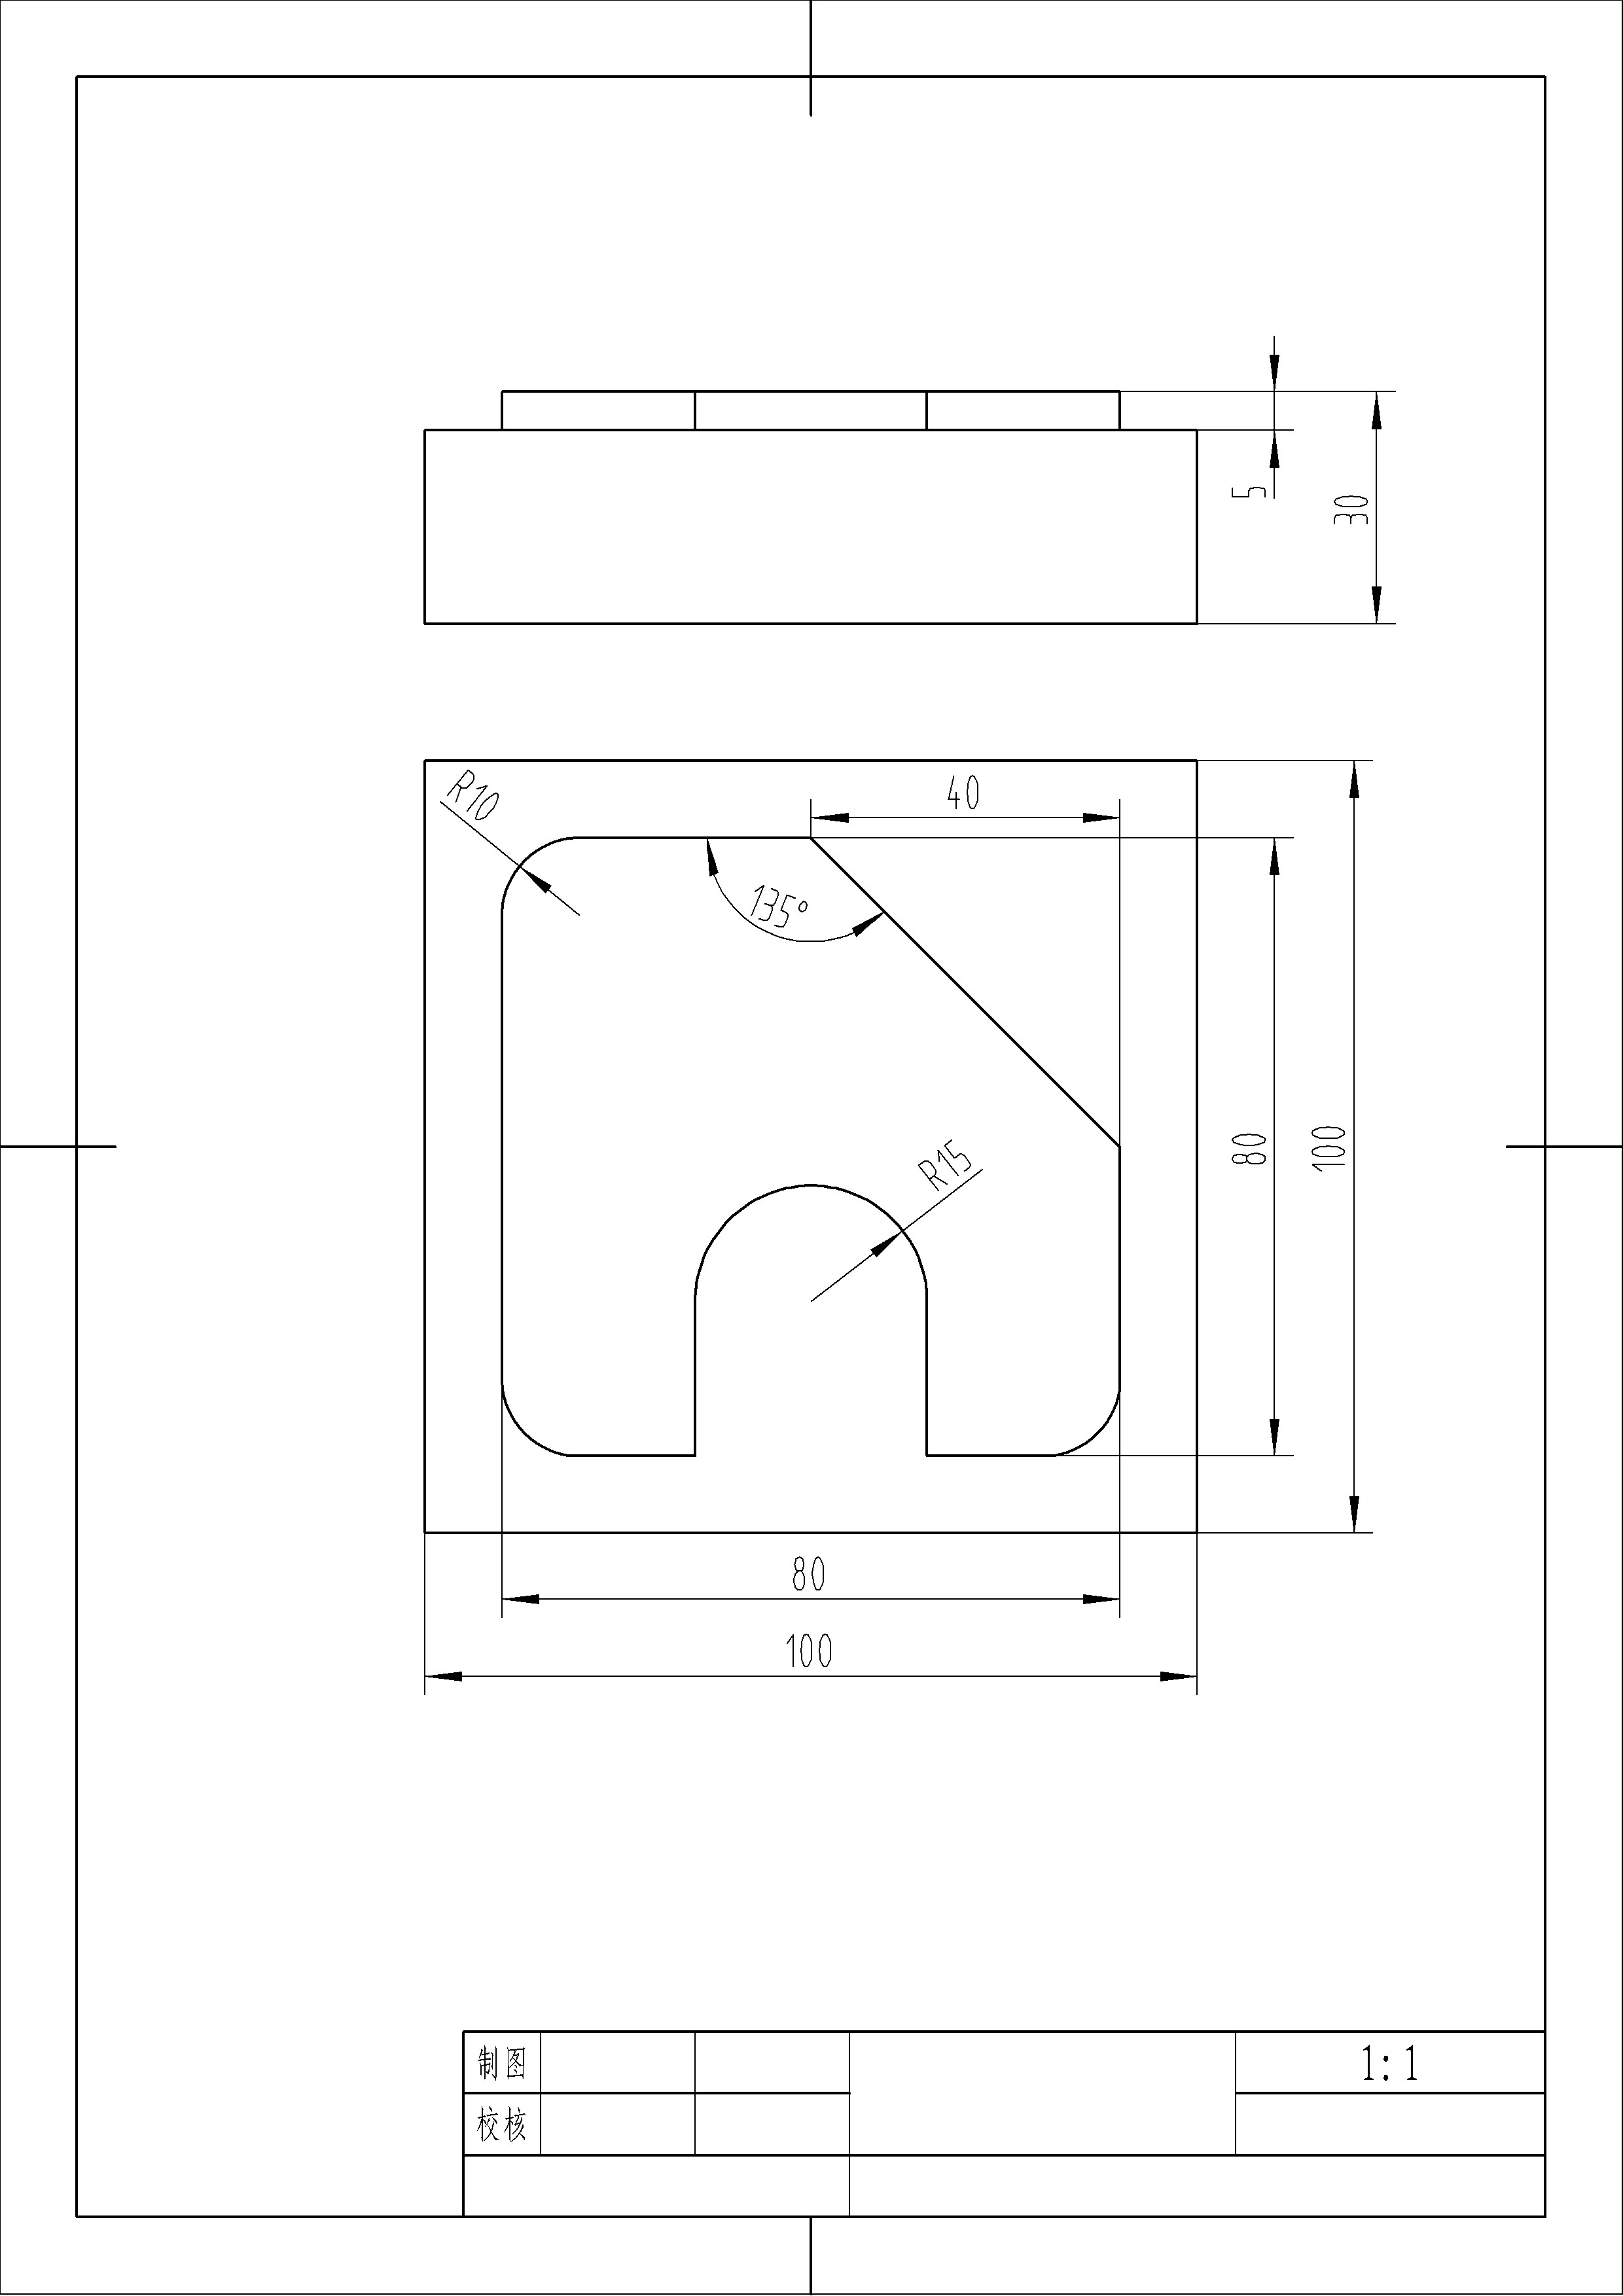
\includegraphics[width=0.8\linewidth,trim=130 200 80  120,clip]{data/image/14-1.jpg}
	\caption{刀补实例}
	\label{fig:14-1}
\end{figure}

1、残料计算:

三个角处的残料为 $20\sqrt{2}-10=18.28$

大角处的残料为  $50\sqrt{2}-20\sqrt{2}=30\sqrt{2}=42.42$

则无论用多大的刀具,此处的残料都不能用刀具半径补偿功能进行去残料。

2、增加刀路去残料:

适合所有类型的去残料,

难点:刀路怎么设计,相关点的计算

基本要求:不能过切,粗加工后能把所有残料去完

自动编程软件:自动计算:

平行往复走刀

沿部件平行环切

沿毛坯平行环切

螺旋高速切削

手工编程:选计算较简单的方法

常用去残料刀路设计:


角

大圆

3、刀路设计:

刀具:铣平面及粗加工:\diameter 12立铣刀

加工宽度10mm

精加工\diameter 10立铣刀

去残料刀路:

角点坐标:

R10--R16.5(粗加工)--R26.5($18.5-16.5=2$)残料去完--改成直线(切线)

$20\sqrt{2}-26.5=2.32$

两边的长:$2.32\sqrt{2} =3.28$

点A(50,-46.)  B(46,-50)

其余根据对称点进行计算

G1 X50. Y-46. 

X46. Y-50.

中间下面的半圆槽:

直线:$C(0,-60) D(0,-20)$


大角:   

$28.28+6.5$ (粗加工) 

$28.28+16.5=44.78$(相当于刀补16.5)

坐标 $ X=50-(70.7-44.78)\sqrt{2} 
=13.349$

$28.28+26.5=54.78 $(相当于刀补26.5)

$X=50-(70.7-54.78)\sqrt{2} 
=27.489$

$28.28+36.6=64.78$(相当于刀补36.5)$+6=42.5$去完

$X=50-(70.7-64.78) \sqrt{2}
=41.629$

G1 X50 Y50

X41.629

X50 Y41.629

Y27.489

X27.489Y50

X13.349

X50 Y13.349

4、程序编写
\begin{lstlisting}

O1(粗加工主程序)
G54G17G40G49G90
M3S500
G1Z20.F2000
X70.Y70.
Z3.0
Z-5. F200
M98P2(去残料)
Z5.0
X0Y60.
Z-5.0
D1M98P3
G1Z30.F2000
M5 
M30
\end{lstlisting}

\begin{lstlisting}
O2(去残料子程序)
N1 G1 X50 Y50
X41.629
X50 Y41.629
Y27.489
X27.489Y50
X13.349
X50 Y13.349
X60.
N2 Y-46.
X50.
X46.Y-50.
Y-60
N3X-46.
Y-50.
X-50.Y-46.
Y-60.
N4 Y46.
X-50
X-46.Y50.
Y60.
M99;
\end{lstlisting}

\begin{lstlisting}
O3(轮廓子程序)
G1X-10.Y50.
G3X0Y40.R10.
G1X40.Y0
G1Y-30.
...

...

\end{lstlisting}












\begin{lstlisting}
O4(精加工主程序)
G54G17G40G49G90
M3S800
G1Z20.F2000
X0.Y60.
Z3.0
Z-5. F200
Z-5.0
D1M98P3
G1Z30.F2000
M5 
M30
\end{lstlisting}




\subsection{课堂小结}
\begin{enumerate}[1、]
	\item 增加刀路去残料;
	\item 加工实例;
	\item 相关计算。
\end{enumerate}

\vfill
\subsection{布置作业}
\begin{enumerate}[1、]
	\item 编写上面的程序。
\end{enumerate}
\vfill
%\jxhj{%教学后记
	}
\skrq{%授课日期
	2017年6月5日 4-5节}
\ktmq{%课题名称
	 综合加工}
\jxmb{%教学目标,每行前面要加 \item
	\item 掌握二维图的绘制;
	\item 掌握挖槽加工参数的设置;
	\item 掌握孔加工参数的设置。}
\jxzd{%教学重点,每行前面要加 \item
	\item 二维图的绘制;
	\item 挖槽加工参数的设置。}
\jxnd{%教学难点,每行前面要加 \item
	\item 挖槽加工参数的设置。}
\jjff{%教学方法
	通过讲述、举例、演示法来说明;}

\makeshouye %制作教案首页

%%%%教学内容
\subsection{组织教学}
\begin{enumerate}[\hspace{2em}1、]
	\item 集中学生注意力;
	\item 清查学生人数;
	\item 维持课堂纪律;
\end{enumerate}
\subsection{复习导入及主要内容}
\begin{enumerate}[1、]
	\item 数据线的接法;
	\item 传输过程;
	\item DNC 在线加工。
\end{enumerate}


\subsection{教学内容及过程}

\subsubsection{绘制图形}
如图\ref{二维图}所示:(数铣的第四个课题图)
\begin{figure}[!hbtp]
	\centering	\includegraphics[width=0.95\textwidth]{images/15-1}
	\caption{二维图} \label{二维图}
\end{figure}

绘图工具的使用

1、	圆弧、圆\par
2、	直线、垂直线、水平线的绘制(与cad不一样)\par
3、	图形的修剪与延伸(分割物体、三个物体修剪、两个物体修剪、一个物体修剪、点修剪)延伸与打断\par
4、	倒圆角(修剪与不修剪)\par
5、	单体补正、串联补正(注意补正的方向,最好标注一下)\par
6、	尺寸的标注,(目的是进行检查)\par
7、	图层的操作(显示与关闭、图素图层的更改)\par
\subsubsection{面铣加工}
如图\ref{面铣加工}所示:
\begin{figure}[!hbtp]
	\centering	\includegraphics[width=0.95\textwidth]{images/15-2}
	\caption{面铣加工} \label{面铣加工}
\end{figure}

1、	机床的选择(三轴立式铣床)\par
2、	机床参数的设定(刀具、毛坯等)\par
3、	面铣操作\par
图素的选择\par
刀具的选择及参数的设定\par
刀具过滤器、刀具号、补偿号、切削用量等\par
切削参数:\par
加工方向:单向、双向、一刀式、动态\par
对刀位置:刀尖、中心\par
两切削间位移方式:\par
底面预留量:\par
参考高度、安全高度、进给下刀位置、工件表面、深度\par
\subsubsection{外形加工}
如图\ref{外形加工}所示:
\begin{figure}[!hbtp]
	\centering	\includegraphics[width=0.95\textwidth]{images/15-3}
	\caption{外形加工} \label{外形加工}
\end{figure}
1、图素的选择\par
2刀具的选择及参数的设定\par
刀具过滤器、刀具号、补偿号、切削用量等\par
3、切削参数:\par
补正方式\par
补正方向\par
刀具在转角处走圆角\par
外形切削方式\par
壁边预留量\par
底边预留量\par
4、参考高度、安全高度、进给下刀位置、工件表面、深度\par
5、Z向分层加工\par
6、XY向分层加工\par
7、切入切出的设定\par
8、切入切出点的设定\par
9、加工方向补偿方向的改变。\par
\subsubsection{刀路的检查与模拟}
1、	二维图形模拟\par
刀具的显示\par
着色显示\par
Z向坐标显示\par
2、	实体验证\par
如图\ref{实体验证}所示:
\begin{figure}[!hbtp]
	\centering	\includegraphics[width=0.95\textwidth]{images/15-4}
	\caption{实体验证} \label{实体验证}
\end{figure}
\subsubsection{应用、完成零件加工、后处理、生成加工程序}
如图\ref{完成零件}所示:
\begin{figure}[!hbtp]
	\centering	\includegraphics[width=0.95\textwidth]{images/15-4}
	\caption{完成零件} \label{完成零件}
\end{figure}	
\subsubsection{其他图形的练习}

自己练习










\subsection{课堂小结}
\begin{enumerate}[1、]
	\item 绘制图形;
	\item 面铣加工;
	\item 外形加工。
\end{enumerate}

\vfill
\subsection{布置作业}
\begin{enumerate}[1、]
	\item 自选图,完成简单零件的自动加工。
\end{enumerate}
\vfill
\biaoti{实习}%标题头
%重新设定目录
%\titlecontents{section}[0pt]{\addvspace{5pt}\filright}
%{ 实习  \thecontentslabel \hspace{0.5em} }
%{}{\titlerule*[8pt]{.} \contentspage}
%\jxhj{%教学后记
	}
\skrq{%授课日期
	2017年6月12日 4-5节}
\ktmq{%课题名称
	 复习}
\jxmb{%教学目标,每行前面要加 \item
	\item 复习相关知识;
	\item 巩固相关知识。}
\jxzd{%教学重点,每行前面要加 \item
	\item 复习相关知识;
	\item 巩固相关知识。}
\jxnd{%教学难点,每行前面要加 \item
	\item 巩固相关知识。}
\jjff{%教学方法
	通过讲述、举例、演示法来说明;}

\makeshouye %制作教案首页

%%%%教学内容
\subsection{组织教学}
\begin{enumerate}[\hspace{2em}1、]
	\item 集中学生注意力;
	\item 清查学生人数;
	\item 维持课堂纪律;
\end{enumerate}
\subsection{复习导入及主要内容}
\begin{enumerate}[1、]
	\item 绘制图形;
	\item 面铣加工;
	\item 外形加工。
\end{enumerate}


\subsection{教学内容及过程}
\subsubsection{小结}
本学期教学工作上的总结,学生学习上的总结,学生作业完成上的总结,学生实习操作上的总结,学生实习报告上的总结,及总体评介,肯定其优点,并指出不足。
\subsubsection{期终考试相关知识}
选择、判断、填空、问答、编程、作图、改错。
\subsubsection{复习基本指令}
G指令\par
G0 G1 G2 G3\par
G17 G18 G19\par
G9 G61 G62 G63 G64\par
G4 \par
G20 G21\par
G40 G41 G42 \par
G43 G44 G49\par
G90 G91\par
G98 G99\par
G81 G82 G83 G84 G85 G86 G87 G88 G89 G80 G73 G74 G76\par
M指令\par
M0 M1 M2 M30\par
M3 M4 M5 M19\par
M6 M7 M8 M9\par
M98 M99\par
其它指令\par
\subsubsection{复习相关知识}
数控加工工艺学\par
数学知识\par
刀具、量具的选择及使用\par
热处理、\par
计算机知识\par
CAD/CAM\par
\subsubsection{复习机床操作知识}\par
操作方式:回零、手动、手轮、MDI、自动、快速、编辑\par
开机\par
手动回参考点\par
手动返回\par
输入程序\par
参数设定\par
程序检查及测试\par
自动加工\par
测量\par
安全:\par
\subsubsection{复习编程思路}
平面\par
外轮廓\par
挖槽(岛屿)\par
孔、\par
凸轮槽\par
薄壁\par
复杂零件\par
配合零件\par
CAD/CAM\par
宏程序\par

\subsection{课堂小结}
\begin{enumerate}[1、]
	\item 小结;
	\item 基本指令;
	\item 相关知识
	\item 机床操作
	\item 编程思路。
\end{enumerate}

\vfill
\subsection{布置作业}
\begin{enumerate}[1、]
	\item 自我复习。
\end{enumerate}
\vfill

\setcounter{section}{0}%重新计数
\ctexset {
	section = {
		name = {实习},
	}
}

\jxhj{%教学后记
}
\skrq{%授课日期
2017~~|~~9.5~~|~~1-3节}
\ktmq{%课题名称
安全操作及机床面板认识}
\jxmb{%教学目标,每行前面要加\item 
\item 明确数控铣/加工中心的文明生产及安全操作规程;
\item 掌握数控铣床/加工中心的组成及坐标系的判定;
\item 明确数控铣床/加工中心MDI面板按键的作用;
\item 掌握回零操作、轴移动操作及开/关机的步骤。}
\jxzd{%教学重点,每行前面要加\item 
\item 明确数控铣床/加工中心MDI面板按键的作用;
\item 掌握回零操作、轴移动操作及开/关机的步骤。}
\jxnd{%教学难点,每行前面要加\item 
\item 掌握回零操作、轴移动操作及开/关机的步骤;}
\jjff{%教学方法
通过讲述、举例、演示法来说明;}

\makeshouye%制作教案首页

%%%%教学内容
\subsection{实习教学要求}
\begin{compactenum}[1、]
\item 明确数控铣/加工中心的文明生产及安全操作规程;
\item 掌握数控铣床/加工中心的组成及坐标系的判定;
\item 明确数控铣床/加工中心MDI面板按键的作用;
\item 掌握回零操作、轴移动操作及开/关机的步骤。
\end{compactenum}

\subsection{相关工艺}
\subsubsection{文明安全生产要求}
\begin{compactenum}[1、]
\item 精神饱满、文明交流;
\item 统一工作服;
\item 操作台只站一个人、在规定的区域里活动;
\item 工件、量具等摆放整齐有序;
\item 精密量具放在盒子里;
\item 爱护机床卫生、保持车间整洁;
\item 严格按机床安全操作规程操作;
\item 禁止修改系统参数;
\item 实行“一人一机上机操作”;
\item 穿合适的工作服,禁止戴手套、穿拖鞋;
\item 女生盘好头发;
\item 加工中禁止离机。
\end{compactenum}


\subsubsection{安全操作规程}\marginpar{具体后面讲解}
\begin{compactenum}[1、]
\item 开机;
\item 程序调试;
\item 加工中;
\item 关机。
\end{compactenum}

\subsubsection{数控铣/加工中心的组成}
\begin{compactenum}[1、]
\item 主轴箱主轴;
\item 控制面板;
\item 电气柜;
\item 立柱床身;
\item 工作台;
\item 冷却液箱;
\item 刀库。
\end{compactenum}

\subsubsection{机床面板及数控系统界面}
\begin{compactenum}[1、]
\item 加工方式:手动、MDI、自动、编辑、回零、DNC等;
\item 进给倍率、快速倍率、主轴倍率;
\item 复位、进给保持、循环启动;
\item 轴移动、主轴正转/反转/停止、切削液开/关、刀库正/反转;
\item 跳段、单段、选择停、空运行、机床锁住、Z轴锁住、M功能锁住;
\item 急停、手轮;
\item 地址键:OPGR……;
\item 数据键:1234……;
\item 功能键:POS、PROG、OFFSETSETING、SYSTEM、MESSAGE、GRAPH;
\item 编辑键:SHIFT、CAN、INPUT、ALTER、INSERT、DELETE、EOB;
\item 坐标显示:绝对、相对、总和等;
\item 程序编辑与管理:程序显示、程序信息、背景编程;
\item 加工参数设定:半径、长度、工件坐标系;
\item 图形模拟;
\item 帮助及报警。
\end{compactenum}

\subsubsection{机床基本操作}
\begin{compactenum}[1、]
\item 开机:开机前检查——外部电源——机床电源——取消急停——复位;
\item 回零:回零方式——调节快速倍率——Z+——X+——Y+——各轴指示灯亮;
\item 手动移动:手动方式——调节进给倍率——X/Y/Z轴;
\item 手轮移动:手轮方式——选择轴——选择倍率——手摇手轮;
\item 快速移动:快速方式——调节快速倍率——X/Y/Z轴。
\end{compactenum}
\textbf{注意:}
\begin{compactenum}[1、]
\item 开机中禁止按任何按键;
\item 开机后确认显示正常、无报警、风扇电机转动正常;
\item 禁止在零点附近回零;
\item 转动手轮不能过快,以不超过5r/s为宜;
\item 手轮倍率应以X100、X10、X1的顺序操作;
\item 移动轴时应先确认好刀具的移动方向;
\item 超程时解除超程。
\end{compactenum}

\subsection{实习内容及过程}

\subsubsection{集合、组织实习}
1、清查学生人数

2、文明安全生产讲解

3、实习内容说明
\subsubsection{开机15分钟}
1、由组长记录机床相关问题

2、开机前检查仔细

3、空转几分钟预热
\subsubsection{机床操作及编程}
1、教师演示基本操作

2、组长安排2人员操作机床(1人操作,1个指导)

3、其他人员自选图形编程

4、每人操作时间不得超过2小时

5、教师巡回指导
\subsubsection{操作点评及工件检测}
1、学生操作感想说明及自评

2、教师提问及点评

3、学生对工件自测

4、教师检测及评分
\subsubsection{准备下课}
1、清洁数控机床

2、正常关机

3、集合教师点评

\subsection{练习题及作业}
\begin{compactenum}[1、]
\item 写出你所操作的机床的主要技术参数。
\item 按X+、Y+工作台向什么方向称动,与坐标系有什么关系,为什么?
\item 数控铣床开机之后为什么要执行回机床参考点的操作?如何操作?
\item 在启动数控铣床前,操作者要做哪些检查?
\item 什么叫“超程”?如何解除超程报警?
\item 在数控铣床运行过程中,当出现异常情况时如何处理
\end{compactenum}

\vfill
\subsection{加工准备与加工要求}
\subsubsection{加工准备}
\begin{enumerate}[1、]
\item 设备:数控铣床、加工中心。
\item 材料:45圆钢(Ф82*50)。
\item  工具:活动扳手,平行垫铁,百分表,其它常用辅具。
\item  
量具:外径千分尺(0~25、100~125,0.01),深度千分尺(0~25,0.01),R规。
\item  刀具:Ф10、Ф16、Ф14立铣刀、Ф64面铣刀。
\item  夹具:三爪自定心卡盘、螺杆压板、平口钳。
\end{enumerate}
\subsubsection{课题评分表}

{\noindent
\begin{figure}[!hbtp]
%\centering
\footnotesize
\hspace{-3.4ex}\renewcommand\arraystretch{1.9}
\begin{tabu}to0.45\textwidth{|cc|c|c|c|c|c|c|}
\hline
\multicolumn{2}{|c|}{工件编号}&\multicolumn{2}{c}{}&
\multicolumn{2}{|c}{总得分}&\multicolumn{2}{|c|}{}\\
\hline
\multicolumn{2}{|c|}{项目与配分}&\parbox{2ex}{序号}&技术要求&配分
&评分标准&\parbox{4ex}{检测记录}&得分\\
\hline
\multicolumn{2}{|c|}{\multirow{2}{*}{\parbox{10ex}{文明生产
			(20\%)}}}&1&工作服&8&未穿禁止进车间并全扣&&\\
\cline{3-8}
&&2&工具、量具摆放整齐&8&不整齐有序全扣&&\\ \cline{3-8}
&&3&其它&4&不守纪律全扣&&\\
\hline

\multicolumn{2}{|c|}{\multirow{1}{*}{\parbox{10ex}{安全操作规程
			(20\%)}}}&4&操作安全&20&酌情扣分&&\\[.3cm] \hline

\multicolumn{2}{|c|}{\multirow{1}{*}{\parbox{10ex}{加工中心组成
			(10\%)}}}&5&说出各部分名称&10&出错一处扣2分&&\\[.3cm]  \hline

\multicolumn{2}{|c|}{\multirow{2}{*}{\parbox{10ex}{面板系统界面
			(20\%)}}}&6&操作面板&10&出错一处扣2分&&\\ \cline{3-8}
&&7&系统界面的认识	&10&出错一处扣2分&&\\ \hline

\multicolumn{2}{|c|}{\multirow{4}{*}{\parbox{10ex}{机床操作
			(30\%)}}}&8&手动、手轮、快速&10&出错一处扣2分&&\\ \cline{3-8}
&&9&点的定位&10&出错一处扣2分&&\\ \cline{3-8}		
&&10&机床操作规范&5&出错一处扣2分&&\\ \cline{3-8}		
&&11&工件刀具装夹	&5&出错一处扣2分&&\\ \hline	

\multicolumn{2}{|c|}{\multirow{2}{*}{\parbox{10ex}{安全文明生产
(倒扣分)}
}}&12&安全操作&倒扣&
\multirow{2}{*}{\parbox{14ex}{安全事故停止操作或酌情扣分}}&&\\
\cline{3-5}\cline{7-8}
&&13&机床整理&倒扣&&&\\
\hline
\end{tabu}
\end{figure}}
\jxhj{%教学后记
	}
\skrq{%授课日期
	2017年 | 3月14日|3月21日|3月28日|4月4日 | 1-3节}
\ktmq{%课题名称
	 六面圆槽加工}
\jxmb{%教学目标,每行前面要加 \item
	\item 掌握槽的下刀方式;
	\item 掌握六面圆槽的加工工艺;
	\item  掌握圆槽的宏程序。}
\jxzd{%教学重点,每行前面要加 \item
	\item 圆槽的宏程序;
	\item 六面圆槽的加工工艺。}
\jxnd{%教学难点,每行前面要加 \item
	\item 圆槽的宏程序。}
\jjff{%教学方法
	通过讲述、举例、演示法来说明;}

\makeshouye %制作教案首页

%%%%教学内容
\subsection{实习教学要求}
\begin{compactenum}[\hspace{2em}1、]
		\item 掌握槽的下刀方式;
	\item 掌握六面圆槽的加工工艺;
	\item  掌握圆槽的宏程序。
\end{compactenum}

\subsection{相关工艺}
\subsubsection{课题内容}
在上一个课题加工的50*50*50的正方体上,每面加工$\phi  45$、$\phi  
35$、$\phi  25$ 的圆槽,深度为5mm。

\subsubsection{平面程序编写}

\begin{lstlisting}
O2
T1M6
#1=0 (初始高度)
#2=5(终止高度)
#3=45-5.5(圆的半径)
G54G17G40G49G90
G1Z30.F2000
X-5Y0
Z5
 F400
N10 #1=#1+0.5
G3X-5Y0I5J0Z-#1
IF[#1LT#2]GOTO10
#3=5
N20#3=#3+0.5
GIX-#3Y0
G3I#3
IF[#3LT#4]GOTO20
G1Z30.F2000
M5
M30
\end{lstlisting}



\subsubsection{平面加工工艺}
\paragraph{加工顺序}
粗加工顺序

精加工顺序
\paragraph{装夹方式}

\paragraph{切削用量}


\subsection{实习内容及过程}

\subsubsection{集合、组织实习}
1、清查学生人数

2、文明安全生产讲解

3、实习内容说明
\subsubsection{开机15分钟}
1、由组长记录机床相关问题

2、开机前检查仔细

3、空转几分钟预热
\subsubsection{机床操作及编程}
1、教师演示基本操作

2、组长安排2人员操作机床(1人操作,1个指导)

3、其他人员自选图形编程

4、每人操作时间不得超过2小时

5、教师巡回指导
\subsubsection{操作点评及工件检测}
1、学生操作感想说明及自评

2、教师提问及点评

3、学生对工件自测

4、教师检测及评分
\subsubsection{准备下课}
1、清洁数控机床

2、正常关机

3、集合教师点评

\subsection{练习题及作业}
\begin{compactenum}[1、]
	\item 小结;
	\item 基本指令;
	\item 相关知识
	\item 机床操作
	\item 编程思路。
\end{compactenum}

\vfill
\subsection{加工准备与加工要求}
\subsubsection{加工准备}
\begin{enumerate}[1、]
	\item 设备:数控铣床、加工中心。
	\item 材料:45圆钢(Ф82*50)。
	\item 工具:活动扳手,平行垫铁,百分表,其它常用辅具。
	\item 
	量具:外径千分尺(0~25、100~125,0.01),深度千分尺(0~25,0.01),R规。
	\item 刀具:Ф10、Ф16、Ф14立铣刀、Ф64面铣刀。
	\item 夹具:三爪自定心卡盘、螺杆压板、平口钳。
\end{enumerate}
\subsubsection{课题评分表}

{\noindent
	%\begin{figure}[!hbtp]
	%	\centering	
	\footnotesize
	\hspace{-3ex} \renewcommand\arraystretch{1.9}
	\begin{tabu} to 0.45\textwidth {|cc|c|c|c|c|c|c|}
		\hline  
		\multicolumn{2}{|c|}{工件编号}  &\multicolumn{2}{c}{} & 
		\multicolumn{2}{|c}{总得分}   & \multicolumn{2}{|c|}{ }   \\ 
		\hline 
		\multicolumn{2}{|c|}{项目与配分} &\parbox{2ex}{序号}  & 技术要求 & 配分 
		& 评分标准 &  \parbox{4ex}{检测记录}& 得分 \\ 
		\hline 
		\multirow{6}{*}{ \parbox{4ex}{工件加工 (80)}} 
		&\multicolumn{1}{|c|}{A面}  & 1 &面铣  & 10& 超差全扣 & & \\ 
		\cline{2-8}  
		&\multicolumn{1}{|c|}{B面}   & 2 &面铣  & 10 & 超差全扣 & & \\ 
		\cline{2-8} 
		&\multicolumn{1}{|c|}{C面}  & 3 &面铣  & 10& 超差全扣 & & \\ 
		\cline{2-8} 
		&\multicolumn{1}{|c|}{D面}   & 4&面铣  & 10 & 超差全扣 & & \\ 
		\cline{2-8}  
		&\multicolumn{1}{|c|}{E面}   & 5&面铣  & 10 & 超差全扣 & & \\ 
		\cline{2-8}  
		&\multicolumn{1}{|c|}{F面}   & 6&面铣  & 10 & 超差全扣 & & \\ 
		\hline 
		\multicolumn{2}{|c|}{\multirow{2}{*}{\parbox{10ex}{程序与工艺
					(10\%)} } }&7 &程序正确合理  & 10 & 每错一处扣2分 &  &  \\ 
		\cline{3-8} 
		&&8&加工工序卡  &10 &不合理每处扣2分  &&  \\ 
		\hline 
		\multicolumn{2}{|c|}{\multirow{2}{*}{\parbox{10ex}{机床操作
					(10\%)}
		} } &9 &机床操作规范  & 10& 出错一次扣2分 &  &  \\ 
		\cline{3-8} 
		&&10&工件刀具装夹  &10  &出错一次扣2分&&  \\ 
		\hline 	
		\multicolumn{2}{|c|}{\multirow{2}{*}{\parbox{10ex}{安全文明生产
					(倒扣分)}
		} } &11 &安全操作  & 倒扣 & 
		\multirow{2}{*}{\parbox{14ex}{安全事故停止操作或酌情扣分}}&  &  \\ 
		\cline{3-5} \cline{7-8} 
		&&12&机床整理  &倒扣  &  &  &\\ 
		\hline 	
\end{tabu} }
%\end{figure}



%\jxhj{%教学后记
	}
\skrq{%授课日期
	2017年 | 4月11日 |4月18日|4月25日  | 1-3节}
\ktmq{%课题名称
	 	工件找正、装夹与对刀、调速}
\jxmb{%教学目标,每行前面要加 \item
	\item 熟练使用百分表找正虎钳及工件;
	\item 能正确的向加工中心刀库放入刀具;
	\item 熟练安全地调节主轴转速;
\item 	正确地用“取中法”进行对刀。}
\jxzd{%教学重点,每行前面要加 \item
	\item 熟练使用百分表找正虎钳及工件;
	\item 正确地用“取中法”进行对刀。}
\jxnd{%教学难点,每行前面要加 \item
	\item 正确地用“取中法”进行对刀。}
\jjff{%教学方法
	通过讲述、举例、演示法来说明;}

\makeshouye %制作教案首页

%%%%教学内容
\subsection{实习教学要求}
\begin{compactenum}[\hspace{2em}1、]
\item 熟练使用百分表找正虎钳及工件;
\item 能正确的向加工中心刀库放入刀具;
\item 熟练安全地调节主轴转速;
\item 	正确地用“取中法”进行对刀。;
\end{compactenum}

\subsection{相关工艺}
\subsubsection{虎钳及工件的找正}
虎钳找正:清洁工作台及虎钳——安装好百分表——使百分表的表头与固定钳口接触——移动X轴——调整虎钳——固定拧紧虎钳——再打表检查。

工件找正:清洁工作台及虎钳——安装好百分表——使百分表的表头与工件接触——移动轴检查——调整工件——固定螺钉压板——再打表检查
	
找正上表面:清洁工作台及虎钳——安装好百分表——使百分表的表头与工件上表接触——移动轴检查——调整工件——固定螺钉压板——再打表检查

注意:找正时,其偏差不能超过0.01-0.02,宁紧后工件或工作台会发生移动,必须再次检查。

\subsubsection{常用夹具}

	螺钉压板:利用T形槽螺栓和压板将工件固定在机床工作台上即可。用百分表等直接找正工件

	机用虎钳:适合形状比较规则的的零件铣削,零件夹紧时要注意控制工件变形和一端钳口上翘

	铣床用卡盘:如三爪卡盘、四爪卡盘等,使用时用 T 形槽螺栓将卡盘固定在机床工作台上即可。

工件在夹具中的安装:

	使待加工面充分暴露在外,考虑机床主轴与工作台面之间的最小距离和刀具的装夹长度,确保在主轴的行程范围内能使工件的加工内容全部完成; 

	夹具在机床工作台上的安装位置必须给刀具运动轨迹留有空间,不能和各工步刀具轨迹发生干涉; 

	夹点数量及位置不能影响刚性。

\subsubsection{加工中心手动换刀过程}
确认刀具和刀柄的重量 

清洁刀柄锥面和主轴锥孔; 

将刀柄的键槽对准主轴端面键垂直伸入到主轴内,不可倾斜; 

右手按下换刀按钮,压缩空气从主轴内吹出以清洁主轴和刀柄,按住此按钮,直到刀柄锥面与主轴锥孔完全贴合后,松开按钮,刀柄即被自动夹紧,确认夹紧后方可松手; 

用手转动主轴检查刀柄是否正确装夹; 

卸刀柄时,先用左手握住刀柄,再用右手按换刀按钮,取下刀柄。 

\subsubsection{主轴的转速的调节} 

	用主轴倍率调节

	用S指令调节

	用带轮、变速箱、电机档位来调节



\begin{table}
		\caption{主轴转速的调节}
		\centering
	\begin{tabular}{|c|c|c|c|c|c|c|c|c|}
		\hline 
		&  \multicolumn{4}{c|}{1}& \multicolumn{4}{c|}{1} \\ 
		\hline 
		& 1 & 2 & 3 & 4 & 1 & 2 & 3 & 4 \\ 
		\hline 
		A&  &  &  &  &  &  &  &  \\ 
		\hline 
		B&  &  &  &  &  &  &  &  \\ 
		\hline 
	\end{tabular} 
\end{table}

\subsubsection{工件坐标系的设定及对刀}
设定工件坐标系的方法

用G54/G59来设置工件坐标系;

用G92来设置工件坐标系;

用G52来设置局部工件坐标系。

极坐标系及坐标系的旋转

常用对刀工具:

寻边器

分中棒

Z轴对刀仪

塞尺、量块

基准棒

“取中法”对刀:

X、Y向对刀 

A.	寻边器测头靠近工件的左侧; 


B.	用手轮使测头接触到工件左侧,记下机床坐标系中的X1坐标值; 

C.	抬起寻边器,让测头靠近工件右侧; 

D.	全手轮使测头接触到工件左侧,记下机床坐标系中的X2坐标值; 

E.	计算其设定值 X=(X1+X2)/2 

F.	同理可测得Y的设定值。

Z向对刀 

A.	安装加工刀具

B.	将Z轴设定器(或固定高度的对刀块)放置在工件上; 

C.	移动刀具,使刀具端面靠近 Z 轴设定器上表面; 

D.	用手轮使刀具端面接触到 Z 轴设定器上表面,直到其指针指示到零位; 

E.	记下机床坐标系中的Z1值,

F.	计算设定值Z=Z1-Z轴对刀仪高度      (坐标系设定在上表面上)

将测得的 X 、 Y 、 Z 值输入到机床G54-G59的参数中。

效验工件坐标系:

A.	在MDI方式下,执行: G54G90G1X0Y0F2000;

B.	检查刀具是不是在工件坐标系的正上方

C.	再执行:Z10.0F200;

D.	检查刀具是不是在其正上方10mm

注意:检查Z轴时,进给倍率先设为0,再用手调节并控制。

	用机内测量法简化“取中法”的计算


\subsection{实习内容及过程}

\subsubsection{集合、组织实习}
1、清查学生人数

2、文明安全生产讲解

3、实习内容说明
\subsubsection{开机15分钟}
1、由组长记录机床相关问题

2、开机前检查仔细

3、空转几分钟预热
\subsubsection{机床操作及编程}
1、教师演示基本操作

2、组长安排2人员操作机床(1人操作,1个指导)

3、其他人员自选图形编程

4、每人操作时间不得超过2小时

5、教师巡回指导
\subsubsection{操作点评及工件检测}
1、学生操作感想说明及自评

2、教师提问及点评

3、学生对工件自测

4、教师检测及评分
\subsubsection{准备下课}
1、清洁数控机床

2、正常关机

3、集合教师点评

\subsection{练习题及作业}
\begin{compactenum}[1、]
	\item 小结;
	\item 基本指令;
	\item 相关知识
	\item 机床操作
	\item 编程思路。
\end{compactenum}

\vfill
\subsection{加工准备与加工要求}
\subsubsection{加工准备}
\begin{enumerate}[1、]
\item 设备:数控铣床、加工中心。
\item 材料:45圆钢($\varnothing$110*35)。
\item 工具:活动扳手,平行垫铁,百分表,其它常用辅具。
\item 量具:外径千分尺(0~25、100~125,0.01),深度千分尺(0~25,0.01),R规。
\item 刀具:$\varnothing$10、$\varnothing$16、$\varnothing$14立铣刀、$\varnothing$64面铣刀。
\item 夹具:三爪自定心卡盘、螺杆压板、平口钳。
\end{enumerate}
\subsubsection{课题评分表}

{\noindent
%\begin{figure}[!hbtp]
%	\centering	
\footnotesize
\hspace{-3.9ex} \renewcommand\arraystretch{1.9}
\begin{tabu} to 0.5\textwidth {|cc|c|c|c|c|c|c|}
	\hline 
\multicolumn{2}{|c|}{工件编号}  &\multicolumn{2}{c}{} & \multicolumn{2}{|c}{总得分}   & \multicolumn{2}{|c|}{ }   \\ 
	\hline 
 \multicolumn{2}{|c|}{项目与配分} &\parbox{2ex}{序号}  & 技术要求 & 配分 & 评分标准 &  \parbox{4ex}{检测记录}& 得分 \\ 
	\hline 
	
 \multicolumn{2}{|c|}{\multirow{3}{*}{\parbox{10ex}{  找正
 		(25\%)} } }&1  &百分表的使用  &7 & 出错一处扣2分 &  &  \\ 
	\cline{3-8} 
&&2&虎钳及工件的找正  &9  &操作不正确全扣  &&  \\ \cline{3-8} 
&&3&工件上表面的找正  &9  &操作不正确全扣  &&  \\
	\hline 
	
 \multicolumn{2}{|c|}{\multirow{2}{*}{\parbox{10ex}{刀具的安装
 		(15\%)}
 } } &4 &刀具的安装  & 7 & 出错一次扣2分 &  &  \\ 
\cline{3-8} 
&&5&刀库中刀具的安装  &8  &出错一次扣2分&&  \\ 
\hline 	

 \multicolumn{2}{|c|}{\multirow{2}{*}{\parbox{10ex}{主轴的调速
			(15\%)}
} } &6 &主轴的转向  & 7 & 出错一次扣2分 &  &  \\ 
\cline{3-8} 
&&7&主轴转速的调节  &8  &出错一次扣2分&&  \\ 
\hline 

 \multicolumn{2}{|c|}{\multirow{3}{*}{\parbox{10ex}{  对刀
			(25\%)} } }&8  &XY向“取中法”对刀  &18 & 操作不正确全扣 &  &  \\ 
\cline{3-8} 
&&9&Z向对刀  &10  &操作不正确全扣  &&  \\ \cline{3-8} 
&&10&寻边器、Z轴对刀仪的使用  &7 &出错一处扣2分  &&  \\
\hline 

 \multicolumn{2}{|c|}{\multirow{2}{*}{\parbox{10ex}{机床操作
			(10\%)}
} } &11 &机床操作规范  & 5 & 出错一次扣2分 &  &  \\ 
\cline{3-8} 
&&12&工件刀具装夹  &5  &出错一次扣2分&&  \\ 
\hline 

 \multicolumn{2}{|c|}{\multirow{2}{*}{\parbox{10ex}{安全文明生产
 		(倒扣分)}
 } } &13  &安全操作  & 倒扣 & \multirow{2}{*}{\parbox{14ex}{安全事故停止操作或酌情扣分}}&  &  \\ 
\cline{3-5} \cline{7-8} 
&&14&机床整理  &倒扣  &  &  &\\ 
\hline 	
\end{tabu} }
%\end{figure}
\vfill
%\jxhj{%教学后记
	}
\skrq{%授课日期
	2017年 | 5月9日 |5月16日|5月23日|5月30日|6月7日| 1-3节}
\ktmq{%课题名称
	 面铣及手动铣削}
\jxmb{%教学目标,每行前面要加 \item
	\item 掌握平面加工工艺;
	\item 掌握平加工程序;
	\item 掌握手动铣削;
    \item 掌握“取中法”的对刀过程。}
\jxzd{%教学重点,每行前面要加 \item
	\item 掌握平加工程序;
	\item 掌握平面加工工艺。}
\jxnd{%教学难点,每行前面要加 \item
	\item 掌握平面加工工艺。}
\jjff{%教学方法
	通过讲述、举例、演示法来说明;}

\makeshouye %制作教案首页

%%%%教学内容
\subsection{实习教学要求}
\begin{enumerate}[1、]
\item 掌握平面加工工艺;
\item 掌握平加工程序;
\item 掌握手动铣削;
\item 掌握“取中法”的对刀过程。
\end{enumerate}


\subsection{相关工艺知识与编程}

\subsubsection{相关键和按钮的功能}
单段:按下后,指示灯亮,在自动加工时按一次循环启动执行一条程序段。

跳步:打开后,机床不执行带“/”的程序段。

空运行:打开此功能后,机床以最快的速度移动,用于校验程序。

机床锁住:开开此功能后,机床仅进行脉冲分配,但不输出脉冲到伺服电机上,即位置显示与程序同步,但机床不移动,M、S、T代码执行。

选择停:打开此功能后,在自动运行时,遇到M01,程序晢停,冷却关断,按“循环启动”继续执行下段程序。

辅助功能锁住:在自动运行时,M、S、T指令不执行。

循环启动:启动加工程序。

进给保持:在自动运行状态下,停止进给,即程序晢停,按循环启动程序接着执行。

Siemens、Fanuc、KND都有此功能按键,位置不同。

\subsubsection{自动运行程序}
1、先对刀,输入好程序

2、选择“自动”方式

3、从存储的程序中选择程序

A、按下[PROG]键,显示程序

B、按下地址[O]键

C、输入程序号

D、按下方向键(向下的)

4、设定好各功能按扭、进给速度等

5、按下[循环启动],程序运行,指示灯亮,程序运行结束,指示灯灭。

6、中途停止或者取消自动运行:

A、用[进给保持],程序晢停

B、按键盘上的复位键,程序结束,机床停止

C、按急停键


\subsubsection{铣平面}

几乎所的有零件都要进行平面铣削,故平面铣削是加工的一项主要内容。

1、采用刀具,一般用面铣刀,其直径为40-250mm螺旋角为10度,刀齿数为10-20个。小平面也可采用大直径的立铣刀。

2、切削深度,铣平面要保证去掉毛坯上的凸凹不平,如要提高表面质量,平面可再铣0.2mm。

3、走刀路径:直线单方向,直线往返,走圆形。
切削宽度:刀具直径的60%-80%

4、工件坐标系原点:

毛坯上表面:(后面的程序Z方向不好计算)

加工后上表面:(下刀到Z0)

5、参考程序:

\begin{lstlisting}
Fanuc:
O0001;
G54G17G40 G90G80;
M03 S300;
G0 X-60. Y-60.0;
Z10.0;
G01 Z0 F100.0;
N10 G01 G91 X120.0 F300.0;
Y10.0;
X-120.0;
Y10.0;
#1=#1+1;
IF [#1 < 6 ] GOTO10;(中间没有空隔)
G90 Z10.0;
G00 Z50.0;
X0 Y0;
M05 
M30
\end{lstlisting}
圆形路径自己写。


\subsubsection{编写程序的基本思路}
程序初始化(安全保护)------辅助准备(换刀、主轴启动、切削液开等) ------提刀到安全平面------定位到下刀点------快速下刀------工进下刀------加工轮廓------提刀-------快速提刀到安全平面-----程序结束(换刀、主轴停止、切削液关、程序返回等)


\subsection{实习内容及过程}

\subsubsection{集合、组织实习}
1、清查学生人数

2、文明安全生产讲解

3、实习内容说明
\subsubsection{开机15分钟}
1、由组长记录机床相关问题

2、开机前检查仔细

3、空转几分钟预热
\subsubsection{机床操作及编程}
1、教师演示基本操作

2、组长安排2人员操作机床(1人操作,1个指导)

3、其他人员自选图形编程

4、每人操作时间不得超过2小时

5、教师巡回指导
\subsubsection{操作点评及工件检测}
1、学生操作感想说明及自评

2、教师提问及点评

3、学生对工件自测

4、教师检测及评分
\subsubsection{准备下课}
1、清洁数控机床

2、正常关机

3、集合教师点评


\vfill
\subsection{加工准备与加工要求}
\subsubsection{加工准备}
\begin{enumerate}[1、]
	\item 设备:数控铣床、加工中心。
	\item 材料:45圆钢($\varnothing$110*35)。
	\item 工具:活动扳手,平行垫铁,百分表,其它常用辅具。
	\item 量具:外径千分尺(0~25、100~125,0.01),深度千分尺(0~25,0.01),R规。
	\item 刀具:$\varnothing$10、$\varnothing$16、$\varnothing$14立铣刀、$\varnothing$64面铣刀。
	\item 夹具:三爪自定心卡盘、螺杆压板、平口钳。
\end{enumerate}
\subsubsection{课题评分表}

{\noindent
%\begin{figure}[!hbtp]
%	\centering	
\footnotesize
\hspace{-2.8ex} \renewcommand\arraystretch{1.9}
\begin{tabu} to 0.5\textwidth {|cc|c|c|c|c|c|c|}
	\hline 
	\multicolumn{2}{|c|}{工件编号}  &\multicolumn{2}{c}{} & \multicolumn{2}{|c}{总得分}   & \multicolumn{2}{|c|}{ }   \\ 
	\hline 
	\multicolumn{2}{|c|}{项目与配分} &\parbox{2ex}{序号}  & 技术要求 & 配分 & 评分标准 &  \parbox{4ex}{检测记录}& 得分 \\ 
	\hline 
	\multirow{4}{*}{ \parbox{4ex}{工件加工 (80)}} &\multicolumn{1}{|c|}{上面}  & 1 &面铣  & 4 & 超差全扣 & & \\ 
	\cline{2-8}  
	&\multicolumn{1}{|c|}{上面}   & 2 &尺寸1  & 12 & 超差全扣 & & \\ 
	\cline{2-8} 
	&\multicolumn{1}{|c|}{上面}  & 3 &尺寸2  & 12& 超差全扣 & & \\ 
	\cline{2-8} 
	&\multicolumn{1}{|c|}{上面}   & 4&椭圆  & 30 & 超差全扣 & & \\ 
	\hline 
	\multicolumn{2}{|c|}{\multirow{2}{*}{\parbox{10ex}{程序与工艺
				(10\%)} } }&5  &程序正确合理  & 5 & 每错一处扣2分 &  &  \\ 
	\cline{3-8} 
	&&6&加工工序卡  &5  &不合理每处扣2分  &&  \\ 
	\hline 
	\multicolumn{2}{|c|}{\multirow{2}{*}{\parbox{10ex}{机床操作
				(10\%)}
	} } &7 &机床操作规范  & 5 & 出错一次扣2分 &  &  \\ 
	\cline{3-8} 
	&&8&工件刀具装夹  &5  &出错一次扣2分&&  \\ 
	\hline 	
	\multicolumn{2}{|c|}{\multirow{2}{*}{\parbox{10ex}{安全文明生产
				(倒扣分)}
	} } &9  &安全操作  & 倒扣 & \multirow{2}{*}{\parbox{14ex}{安全事故停止操作或酌情扣分}}&  &  \\ 
	\cline{3-5} \cline{7-8} 
	&&10&机床整理  &倒扣  &  &  &\\ 
	\hline 	
\end{tabu} }
%\end{figure}
\vfill

\newpage
\newgeometry{top=2cm, bottom=2cm, left=2.cm, right=2.cm,includehead,includefoot}
\fancyhead{} 
\chead{ }
\lhead{ } %边框 
\rhead{ }%边框 
\zihao{-4}	

\newpage 
%\begin{figure}[!h]
%	\centering	
%	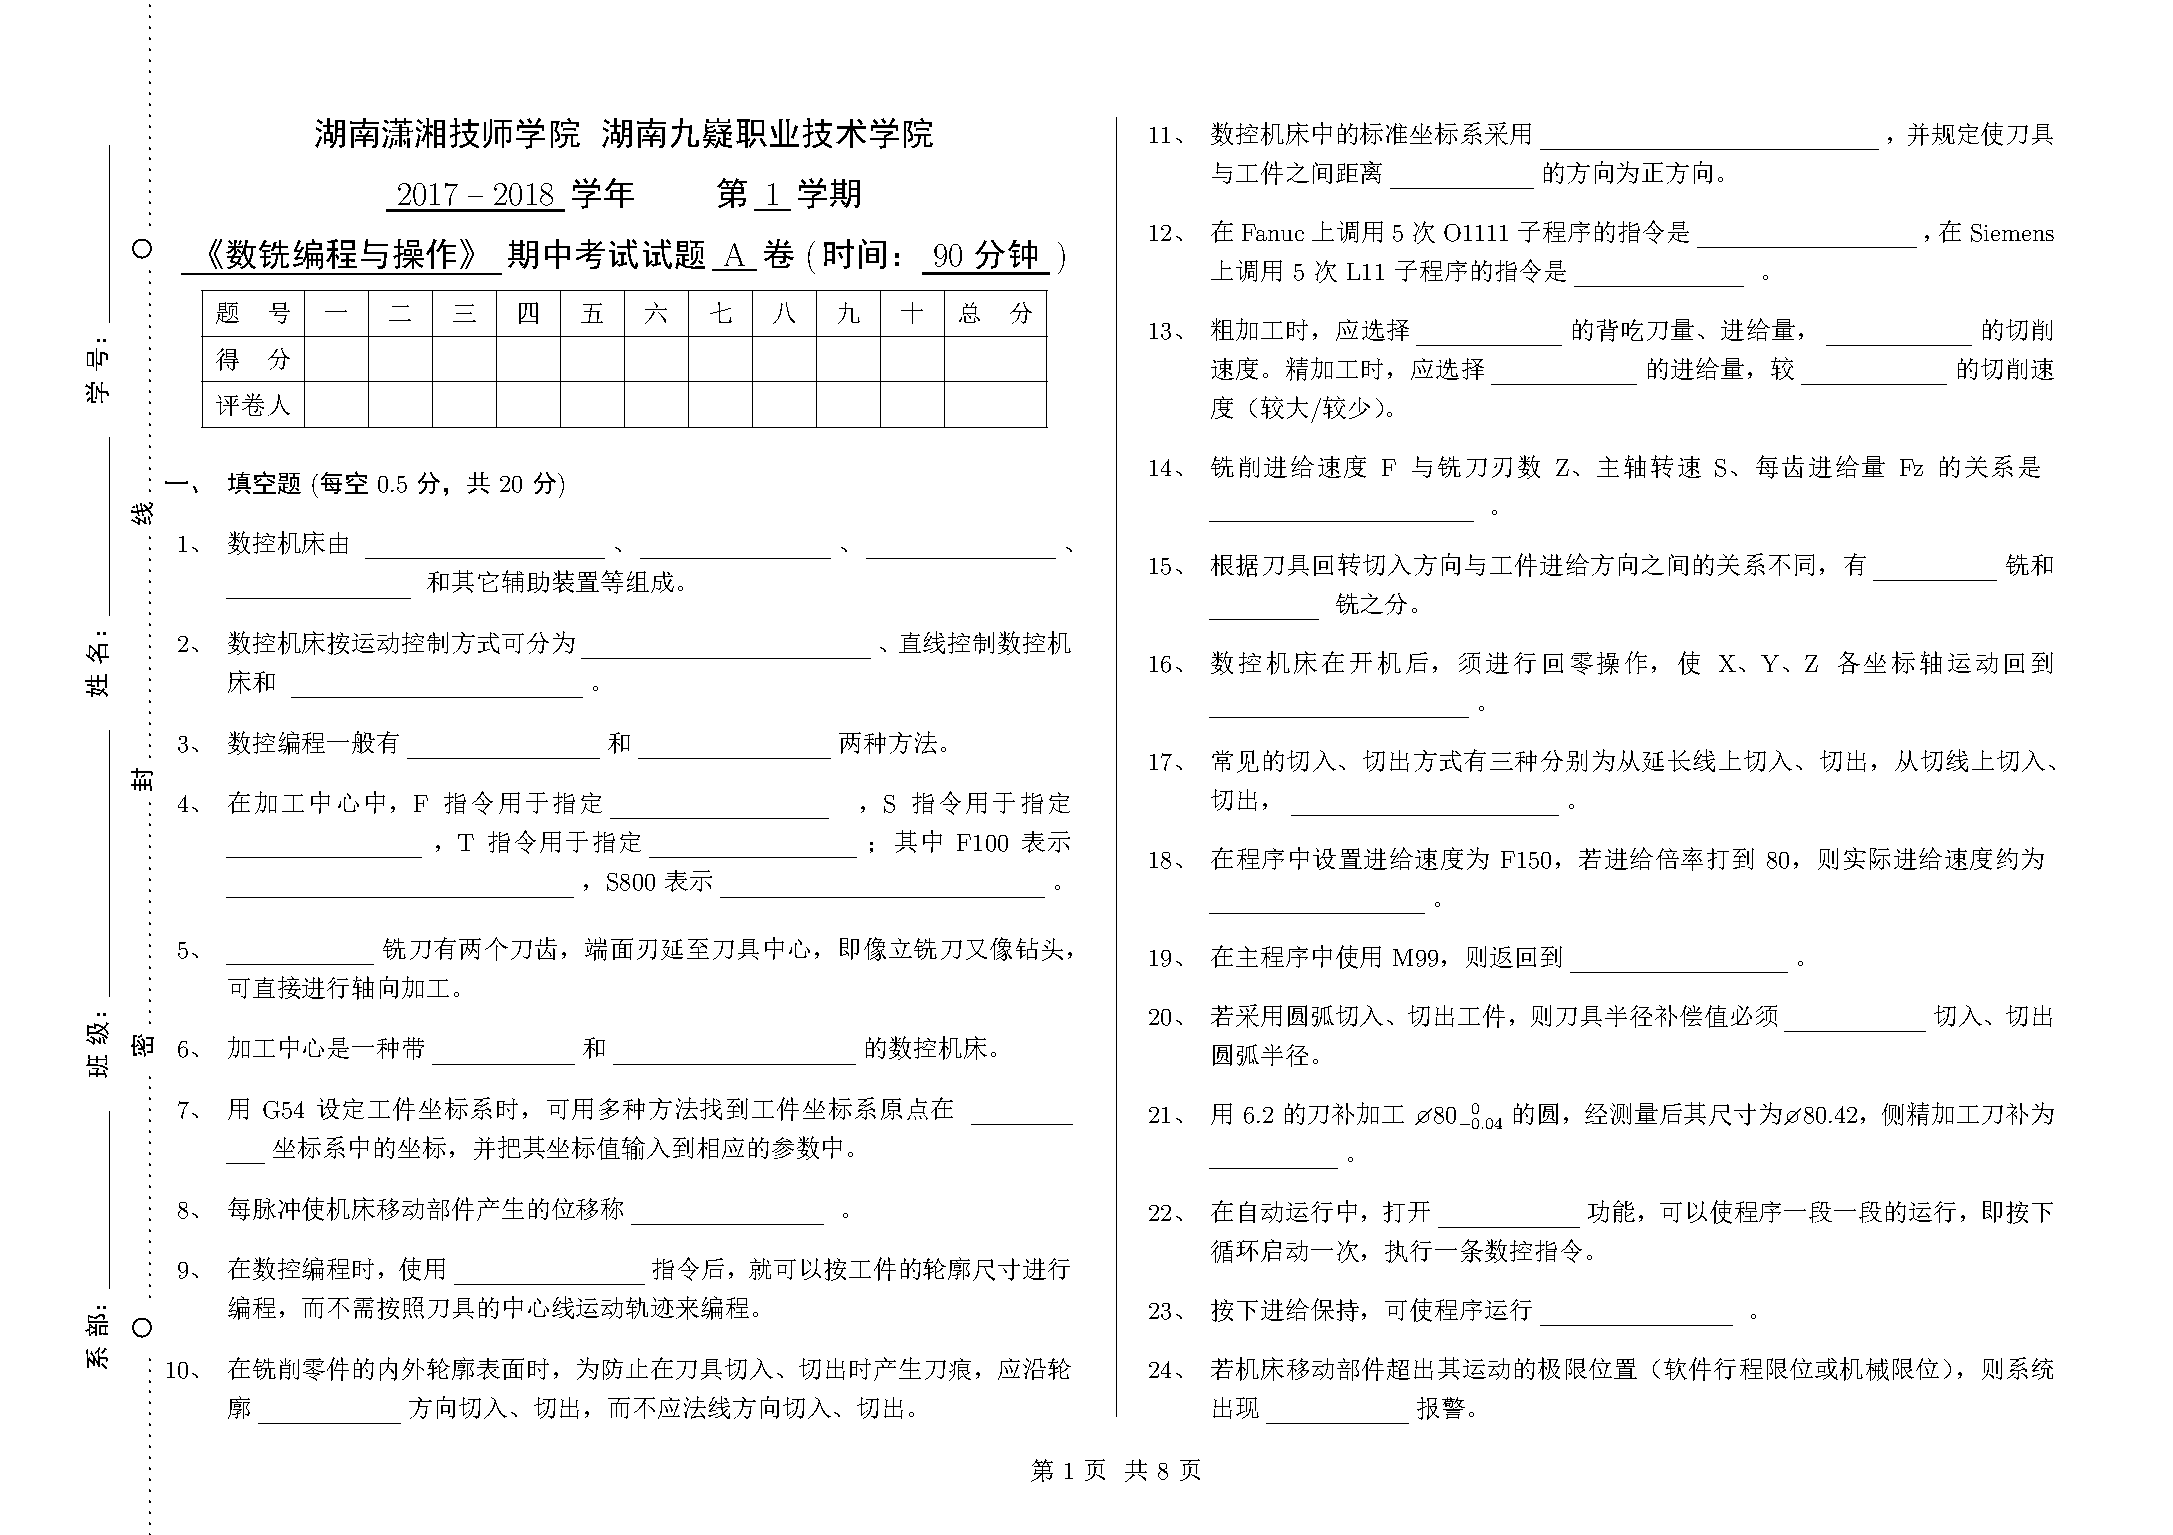
\includegraphics[height=\textwidth,angle=90]{images/shijuan1}
%\end{figure}
%\begin{figure}[!h]
%	\centering	
%	\includegraphics[height=\textwidth,angle=90]{images/shijuan2}
%\end{figure}
%\begin{figure}[!h]
%	\centering	
%	\includegraphics[height=\textwidth,angle=90]{images/shijuan3}
%\end{figure}
%\begin{figure}[!h]
%	\centering	
%	\includegraphics[height=\textwidth,angle=90]{images/shijuan4}
%\end{figure}

%\newpage
%\begin{figure}[!h]
%	\centering	
%	\includegraphics[width=0.9\textwidth,angle=0]{images/fenshu1}
%\end{figure}
%\begin{figure}[!h]
%	\centering	
%	\includegraphics[width=0.9\textwidth,angle=0]{images/fenshu2}
%\end{figure}
%\begin{figure}[!h]
%	\centering	
%	\includegraphics[width=0.9\textwidth,angle=0]{images/fenshu3}
%\end{figure}
%\begin{figure}[!h]
%	\centering	
%	\includegraphics[width=0.9\textwidth,angle=0]{images/fenshu4}
%\end{figure}
%\begin{figure}[!h]
%	\centering	
%	\includegraphics[width=0.9\textwidth,angle=0]{images/fenshu5}
%\end{figure}
%\begin{figure}[!h]
%	\centering	
%	\includegraphics[width=0.9\textwidth,angle=0]{images/fenshu6}
%\end{figure}
%\begin{figure}[!h]
%	\centering	
%	\includegraphics[width=0.9\textwidth,angle=0]{images/fenshu7}
%\end{figure}
%\begin{figure}[!h]
%	\centering	
%	\includegraphics[width=0.9\textwidth,angle=0]{images/fenshu8}
%\end{figure}
%
%\newgeometry{top=2cm, bottom=1.5cm, left=2cm, right=2cm,includefoot}
%\newpage
%%\documentclass[UTF8,zihao=5,linespread=1 ]{ctexart}
%\usepackage[papersize={210mm,276mm},top=2cm, bottom=1cm, left=2cm, right=2cm,includefoot]{geometry}
%\usepackage[utf8]{inputenc}
%\usepackage{amsmath}
%\usepackage{amsfonts}
%\usepackage{amssymb}
%\usepackage{makeidx}
%\usepackage{graphicx}
%\usepackage{tabu}
%\usepackage{tikz}
%
%%\usepackage{colortbl}
%\usepackage{arydshln}
%\usepackage{multirow}
%%\usepackage{multicol}
%
%
%\pagestyle{empty}


%\author{高星}
%\title{试卷分析}
{
\newcommand{\ul}[2]{\underline{\makebox[#1]{\heiti #2}}}
%\newcolumntype{M}[1]{>{\sihao\centering\arraybackslash}m{#1}}
\newcolumntype{N}{@{}m{0pt}@{}}
%\begin{document}
\begin{center}
		{\LARGE \heiti 湖南潇湘技师学院 \hspace{1cm} 考试情况分析表 } \\[0.5cm]
{\scriptsize 
   \begin{tabu} to \textwidth 
   	   {|X[2,c,m]|X[1,c,m]|X[1,c,m]|X[1,c,m]|X[1,c,m]
   		|X[1,c,m]|X[1, l,m]|X[1,c,m]|X[1,c,m]|X[1,c,m]
   		|X[1,c,m]|X[2.8,c,m]|X[1,c,m]|X[2.8,c,m]|X[2.2,l,m]
   		|X[2.2,c,m]|X[2.2,c,m]|N} 
   	\hline 
%    1&2&3&4&5&6&7&8&9&10&11&12&13&14&15&16&17&\\[0.6cm]\hline 
    班级&\multicolumn{3}{c|}{16级大专模具}&学科&\multicolumn{3}{c|}{数铣理论}&\multicolumn{2}{c|}{全班人数}&30&实考人数&30&任课教师&高星&班主任&庄荣&\\[0.5cm]\hline 
    分数段&0-9&10-19&20-29&30-39&40-49&50-59&60-69&70-79&90-89&90-100&\multicolumn{6}{c|}{\multirow{8}{*}{
\begin{tikzpicture}[x=1cm,y=0.5cm]
\draw[xstep=0.5cm,ystep=0.25cm,gray,very thin] (0,0) grid (5,5);
\draw
(0,-0.3) node {0}
(0.5,-0.3) node {1}
(1,-0.3) node {2}
(1.5,-0.3) node {3}
(2,-0.3) node {4}
(2.5,-0.3) node {5}
(3,-0.3) node {6}
(3.5,-0.3) node {7}
(4,-0.3) node {8}
(4.5,-0.3) node {9}
(5,-0.3) node {10}
(5.8,0) node {成绩序号}
(-0.3,0) node {0}
(-0.3,0.5) node {1}
(-0.3,1) node {2}
(-0.3,1.5) node {3}
(-0.3,2) node {4}
(-0.3,2.5) node {5}
(-0.3,3) node {6}
(-0.3,3.5) node {7}
(-0.3,4) node {8}
(-0.3,4.5) node {9}
(-0.3,5) node {10}
(-0.2,5.8) node {人数}
(2.5,6) node {\heiti \normalsize  成~绩~分~布~图}
;
\filldraw (0,0)circle(2pt)--(0.5,0)circle(2pt)--(1,0)circle(2pt)--
(1.5,1)circle(2pt)--(2,1)circle(2pt)--(2.5,2)circle(1pt)--
(3,1.5)circle(2pt)--(3.5,3.5)circle(2pt)--(4,2.5)circle(2pt)--
(4.5,1.5)circle(2pt)--(5,0)circle(2pt);
\end{tikzpicture}
}}&\\[0.6cm]\cline{1-11}
    人数&0&0&0&2&2&3&7&5&3&0&\multicolumn{6}{c|}{}&\\[0.5cm]\cline{1-11}
    \%&8.8&5.9&11.8&11.8&5.9&5.9&5.9&5.9&8.8&26.5&\multicolumn{6}{c|}{}&\\[0.5cm]\cline{1-11}
    人数&&&&&&&&&&&\multicolumn{6}{c|}{}&\\[0.5cm]\cline{1-11}
    \%&&&&&&&&&&&\multicolumn{6}{c|}{}&\\[0.5cm]\cline{1-11}
    人数&&&&&&&&&&&\multicolumn{6}{c|}{}&\\[0.5cm]\cline{1-11}
    \%&&&&&&&&&&&\multicolumn{6}{c|}{}&\\[0.5cm]\cline{1-11}
    平均成绩&\multicolumn{4}{c|}{68}&\multicolumn{2}{c|}{及格率}&\multicolumn{4}{c|}{64.7\%}&\multicolumn{6}{c|}{}&\\[0.5cm]\hline
    题号&\multicolumn{2}{c|}{题型}&\multicolumn{3}{c|}{试题检查目的}&\multicolumn{6}{c|}{学生知识掌握情况}&\multicolumn{2}{c|}{分析原因}&\multicolumn{3}{c|}{改进措施}&\\[0.5cm]\hline
    一&\multicolumn{2}{c|}{图样分析}&\multicolumn{3}{c|}{\multirow{1}{7em}{检查学生三维空间想象的能力,图样公差精度的分析能力。}}&\multicolumn{6}{c|}{\multirow{1}{19.5em}{大部分同学掌握很好,少数同学没有掌握;有些同学没有注意到未注公差。}}&\multicolumn{2}{c|}{\multirow{1}{7em}{有些同学没有掌握,练习少。}}&\multicolumn{3}{c|}{多问,多做题、多思考。}&\\[1.5cm]\hline
    二&\multicolumn{2}{c|}{工艺分析}&\multicolumn{3}{c|}{\multirow{1}{7em}{检查学生工艺知识,工艺分析的能力。}}&\multicolumn{6}{c|}{\multirow{1}{19.5em}{大部分同学掌握很好,少数同学没有掌握。}}&\multicolumn{2}{c|}{\multirow{1}{7em}{有些同学没有掌握,练习少。}}&\multicolumn{3}{c|}{多问,多做题、多思考。}&\\[1.5cm]\hline
    三&\multicolumn{2}{c|}{程序编制}&\multicolumn{3}{c|}{\multirow{1}{7em}{检查学生编程指令的使用,编程思路的合理性。}}&\multicolumn{6}{c|}{\multirow{1}{19.5em}{大部分同学掌握很好,少数同学没有掌握。}}&\multicolumn{2}{c|}{\multirow{1}{7em}{有些同学没有掌握,练习少。}}&\multicolumn{3}{c|}{多问,多做题、多思考。}&\\[1.5cm]\hline
    四&\multicolumn{2}{c|}{零件加工}&\multicolumn{3}{c|}{\multirow{1}{7em}{检查学生机床使用,零件加工的相关知识。}}&\multicolumn{6}{c|}{\multirow{1}{19.5em}{大部分同学掌握很好,少数同学没有掌握。}}&\multicolumn{2}{c|}{\multirow{1}{7em}{有些同学没有掌握,练习少。}}&\multicolumn{3}{c|}{多问,多做题、多思考。}&\\[1.5cm]\hline
    五&\multicolumn{2}{c|}{\multirow{1}{4em}{检验与质量分析}}&\multicolumn{3}{c|}{\multirow{1}{7em}{检查学生量具的使用,零件质量分析的相关知识。}}&\multicolumn{6}{c|}{\multirow{1}{19.5em}{大部分同学掌握很好,少数同学没有掌握。}}&\multicolumn{2}{c|}{\multirow{1}{7em}{有些同学没有掌握,练习少。}}&\multicolumn{3}{c|}{多问,多做题、多思考。}&\\[1.5cm]\hline
    \multicolumn{3}{|c|}{总体评价}&\multicolumn{14}{l|}{2/3的同学掌握了所学的知识,1/3的同学有待加强,达到教学目标。}&\\[1cm]\hline 
   \end{tabu} 
}				
\end{center}
\footnotesize
注:1、不同题号的区别横线由老师加画。

 2、考试结束后一周内由任课老师完成分析,一式两份,一份教师留存,一份由教研组长汇总或由任课教师直接交教务处。
}
%\end{document}
%
%\newpage
%\begin{center}
\large \hei 15~级~中~数~班 ~~平~时~成~绩
\renewcommand\arraystretch{1.9}

\song \scriptsize 
\begin{tabu} to \textwidth {|X[1,c,m]|X[6,c,m]|X[2,c,m]|X[1,c,m]|X[1,c,m]|
		X[1,c,m]|X[1,c,m]|X[1,c,m]|X[1,c,m]|X[1,c,m]|
		X[1,c,m]|X[1,c,m]|X[1,c,m]|X[1,c,m]|X[1,c,m]|
		X[1,c,m]|N}
	\hline
序号&学生学号&学生名称&课题1&课题2
&课题3&课题4&实习报告&考勤&作业
&理论平时成绩&理论期末成绩&理论综合成绩&实习平时成绩&实习期末成绩
&实习综合成绩&\\ \hline
1&4305820150910708&唐文杰&97 &97 &97 &97 &97 &99&99&99 
&99&99 &97&91&94&\\ \hline
3&4305820150910710&周洋&80 &80 &80 &80 &80 &48 &48 &48 &23&38 
&80&44&65&\\ \hline
5&4305820150910712&周庚文&80 &80 &80 &80 &80 &35 &35 &35 
&12&26 &80&44&65&\\ \hline
6&4305820150910713&易合金&97 &97 &97 &97 &97 &95 &95 &95 
&90&93 &97&77&89&\\ \hline
7&4305820150910714&胡琴&96 &96 &96 &96 &96 &95 &95 &95 &90&93 
&96&83&90&\\ \hline
8&4305820150910715&乐旭峰&79 &79 &79 &79 &79 &89 &89 &89 
&80&86 &79&44&65&\\ \hline
9&4305820150910716&唐智杰&88 &88 &88 &88 &88 &93 &93 &93 
&86&90 &88&46&71&\\ \hline
15&4305820150910722&周耀华&79 &79 &79 &79 &79 &77 &77 &77 
&60&70 &79&44&65&\\ \hline
16&4305820150910723&王鹏&90 &90 &90 &90 &90 &74 &74 &74 
&55&66 &90&44&71&\\ \hline
17&4305820150910724&黄引亚&88 &88 &88 &88 &88 &84 &84 &84 
&70&78 &88&44&70&\\ \hline
18&4305820150910725&彭杰&79 &79 &79 &79 &79 &0 &0 &0 &0&0 
&79&44&65&\\ \hline
19&4305820150910726&何紫辉&87 &87 &87 &87 &87 &92 &92 &92 
&85&89 &87&50&72&\\ \hline
21&4305820150910728&唐雅红&97 &97 &97 &97 &97 &96 &96 &96 
&92&94 &97&70&86&\\ \hline
22&4305820150910729&唐志成&90 &90 &90 &90 &90 &79 &79 &79 
&63&73 &90&50&74&\\ \hline
24&4305820150910731&乌国勇&88 &88 &88 &88 &88 &75 &75 &75 
&38&60 &88&50&72\\ \hline
25&4305820150910732&马建新&88 &88 &88 &88 &88 &70 &70 &70 
&44&60 &88&52&73&\\ \hline
28&4305820150910735&匡曾铮&88 &88 &88 &88 &88 &84 &84 &84 
&71&79 &88&60&76&\\ \hline
29&4305820150910736&欧斌&80 &80 &80 &80 &80 &42 &42 &42 
&18&33 &80&44&65&\\ \hline
30&4305820150910737&欧军&79 &79 &79 &79 &79 &48 &48 &48 
&23&38 &79&44&65&\\ \hline
31&4305820150910738&彭弘钢&97 &97 &97 &97 &97 &99 &99 &99 
&99&99 &97&90&94&\\ \hline
32&4305820150910739&唐洋&88 &88 &88 &88 &88 &75 &75 &75 
&41&61 &88&44&70&\\ \hline
33&4305820150910740&杨星星&97 &97 &97 &97 &97 &98 &98 &98 
&97&98 &97&83&91&\\ \hline
34&4305820150910741&谢婷婷&97 &97 &97 &97 &97 &95 &95 &95 
&90&93 &97&77&89&\\ \hline
37&4305820150910744&欧阳旭&88 &88 &88 &88 &88 &73 &73 &73 
&54&66 &88&44&70&\\ \hline
38&4305820150910745&黄志扬&89 &89 &89 &89 &89 &60 &60 &60 
&36&50 &89&60&77&\\ \hline
39&4305820150910746&曾德胜&88 &88 &88 &88 &88 &79 &79 &79 
&63&73 &88&66&79&\\ \hline
40&4305820150910747&吴旭东&89 &89 &89 &89 &89 &47 &47 &47 
&22&37 &89&54&75&\\ \hline
41&4305820150910748&徐依建&96 &96 &96 &96 &96 &95 &95 &95 
&90&93 &96&86&92&\\ \hline
42&4305820150910749&何荣云&89 &89 &89 &89 &89 &28 &28 &28 
&8&20 &89&63&78&\\ \hline
43&4305820150910750&郑云翔&89 &89 &89 &89 &89 &0 &0 &0 &0&0 
&89&50&73&\\ \hline
44&4305820150910751&唐家华&81 &81 &81 &81 &81 &58 &58 &58 
&34&49 &81&44&66&\\ \hline
46&4305820150910753&熊文胜&87 &87 &87 &87 &87 &56 &56 &56 
&31&46 &87&48&71&\\ \hline
50&4305820150910757&朱益明&80 &80 &80 &80 &80 &45 &45 &45 
&20&35 &80&44&65&\\ \hline
52&4305820150910931&高新志&96 &96 &96 &96 &96 &98 &98 &98 
&96&97 &96&87&92&\\ \hline
\end{tabu}

\end{center}
%
%\newpage
%\renewcommand{\baselinestretch}{1.3}
%{
%\begin{center}
%	\huge \hei 教 ~ 学  ~总  ~结
%\end{center}
%
% \large  \setlength{\parindent}{2em} 
% 
%《加工中心编程、仿真与操作》是15级中数班的一门专业课,
% 本课程已在上一学期中,就学习了手工编程的基本知识。
% 本学期主要学习简化编程与宏程序,及常见零件的加工工艺。
% 通过本学期的教学,完成了教学任务,基本达到教学目标,教学效果较好。
%
%本学期实习课共分4个课题,都在计划的时间内完成课题的实施,
%有少同学没有完成课题。通过期末考试,大部分的同学掌握的比较好,
%也就是2/3的同学掌握了所学的知识。实习大部分同学完成了课题,
%达到教学目标,教学效果较好。
%
%本学的仿真课主要学习《MasterCAM》自动编程,
%包括二维绘图,二维加工,三维空间曲线,三维曲面及实体,三维加工,
%以及每个课题的仿真模拟等。完成的全部教学。
%
%本学期在教学过程中主要的所用的教学方法为分析引导,
%通过实例进行讲解,仿真与实习相互融通。在进行宏程序入门教学过程中,
%进行实例设计,引导学生进行学习,效果好,工艺课在教学中要多讨论,
%实习课中要引导学生进行自我总结。
%
%在教学中有部分学生厌学,旷课需要进行一步的提高学生们的兴趣,
%在仿真课上,学生们的自觉性较差时,最好安排课题让学生们做。
%要进一步的加强教学管理,并及时与班主任进行联系,沟通。
%以便取得更好的教学效果。
%
%}
%
%
%\newpage
%\pagestyle{empty}
%\begin{center}
%	\huge \hei 教 ~~学 ~~检 ~~查 ~~记~~ 录
%	
%	\song\normalsize 
%	\begin{tabu} to \textwidth {|X[1,c,m]|X[10,r,m]|N}
%		\hline
%	\multirow{1}{1em}{\large 系部意见}  &\vspace{7cm}  检查人签名(盖章) 
%	\hspace{4cm} \par  二〇 \underline{\hspace{2em}}   
%	年\underline{\hspace{1em}}   月 \underline{\hspace{1em}}  日 
%	\hspace{1cm}  \par &\\ [8cm] \hline
%	\multirow{1}{1em}{\large 教务处意见} & \vspace{7cm}  检查人签名(盖章) 
%	\hspace{4cm} \par  二 〇  \underline{\hspace{2em}} 年  
%	\underline{\hspace{1em}} 月 \underline{\hspace{1em}}  日 \hspace{1cm} 
%	\par & \\[8cm] \hline	
%	\end{tabu}
%\end{center}
%



%中文习惯是设定首行缩进为2em。注意此设置一定要在document环境之中,这可能与setlength 作用范围相关
%\setlength{\parindent}{2em}                    
%
%\title{Xecjk Template Test}
%\author{Xiao Hanyu}
%\maketitle
%
%\tableofcontents
%\listoffigures
%%\listoftablescontent
%
%\section{基本文字测试}
\label{sec:1}
我叫肖晗宇,来自浙江大学计算机学院,热爱开源软件、旅行、摄影,推崇互助共享的精神理念。

My name is Xiao Hanyu, a student from Computer Science and Technology of Zhejiang University, I love open source software, travelling all over the world, photography, and so on. 

我喜欢\LaTeXe,也推荐大家来学习使用\LaTeXe,以下是比较不错的学习资源:

\begin{enumerate}
\item LaTeX companion
\item The TeXbook
\end{enumerate}


\section{图形图像测试}
\subsection{插图测试}
Hand in Hand:\ref{fig:hand_in_hand}
\begin{figure}[htbp]
\centerline{\includegraphics[width=0.6\textwidth]{images/hand_in_hand.png}}
\caption[]{\label{fig:hand_in_hand} 手拉手}
\end{figure}

\subsection{pgf/tikz绘图测试}
图\ref{fig:monotonic_chain}是用pgf/tikz宏包作的图形,用以说明计算几何相关定理。

\begin{figure}
\centering
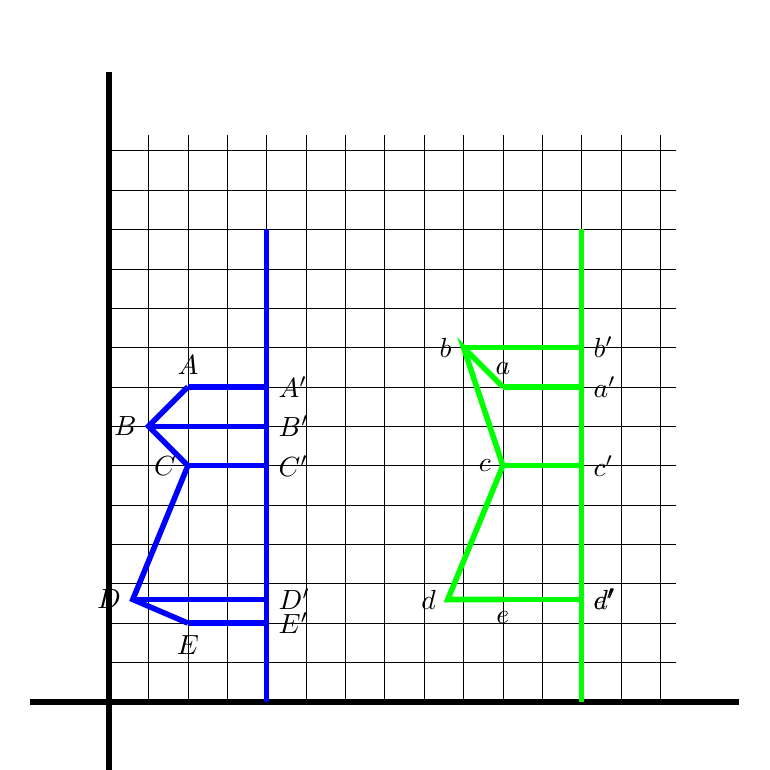
\begin{tikzpicture}[line width=2pt]
\draw (-1,0) -- (8,0);
\draw (0,-1) -- (0,8);
\draw[step=.5cm, very thin] (0,0) grid (7.2,7.2);

\coordinate [label=above:$A$] (A) at (1, 4);
\coordinate [label=left:$B$] (B) at (0.5, 3.5);
\coordinate [label=left:$C$] (C) at (1, 3);
\coordinate [label=left:$D$] (D) at (0.3, 1.3);
\coordinate [label=below:$E$] (E) at (1, 1);

\draw[blue] (A) -- (B) -- (C)  -- (D) -- (E);
\draw[blue] (2, 0) -- (2, 6);

\coordinate [label=right:$A'$] (A') at (2, 4);
\coordinate [label=right:$B'$] (B') at (2, 3.5);
\coordinate [label=right:$C'$] (C') at (2, 3);
\coordinate [label=right:$D'$] (D') at (2, 1.3);
\coordinate [label=right:$E'$] (E') at (2, 1);

\draw[blue] (A) -- (A');
\draw[blue] (B) -- (B');
\draw[blue] (C) -- (C');
\draw[blue] (D) -- (D');
\draw[blue] (E) -- (E');

\coordinate [label=above:$a$] (a) at (5, 4);
\coordinate [label=left:$b$] (b) at (4.5, 4.5);
\coordinate [label=left:$c$] (c) at (5, 3);
\coordinate [label=left:$d$] (d) at (4.3, 1.3);
\coordinate [label=below:$e$] (e) at (5, 1.3);

\draw[green] (a) -- (b) -- (c)  -- (d) -- (e);
\draw[green] (6, 0) -- (6, 6);

\coordinate [label=right:$a'$] (a') at (6, 4);
\coordinate [label=right:$b'$] (b') at (6, 4.5);
\coordinate [label=right:$c'$] (c') at (6, 3);
\coordinate [label=right:$d'$] (d') at (6, 1.3);
\coordinate [label=right:$e'$] (e') at (6, 1.3);

\draw[green] (a) -- (a');
\draw[green] (b) -- (b');
\draw[green] (c) -- (c');
\draw[green] (d) -- (d');
\draw[green] (e) -- (e');
\end{tikzpicture}
\caption{Monotonic polygonal chains}
\label{fig:monotonic_chain}
\end{figure}

\section{表格测试}
\begin{table}[htbp]
  \centering
  \begin{tabular}[htbp]{r|l}
    \toprule
    日期 & 任务 \\
    \midrule
    2011.5 & 完善此份文档 \\
    2011.6 & 完善安装脚本 \\
    \bottomrule
  \end{tabular}
  \caption{表格}
  \label{tab:table1}
\end{table}

\section{源代码高亮测试}

以下是\href{http://acm.zju.edu.cn/onlinejudge/showProblem.do?problemCode=1372}{ZOJ 1372}的解题c++代码:

\begin{lstlisting}[language=c++]
#include <iostream>
#include <string>
using namespace std;
 
const long max_points = 100;
const long infinity = 1000001;
 
int p, r, length, g[max_points][max_points];
bool flag;
 
class vertex
{
public:
    int distance;
    bool visited;
};
 
vertex v[max_points];
 
void initial()
{
    for(int i = 1; i <= p; i++)
        for(int j = 1; j <= p; j++)
            g[i][j] = infinity;
}
 
void prim(int origin)
{
    int temp_min;
    int temp_v = 0;
    int sum = 0;
 
    for(int i = 1; i <= p; i++)
    {
        v[i].distance = g[i][origin];
        v[i].visited = false;
    }
 
    v[origin].distance = 0;
    v[origin].visited = true;
 
    sum++;
 
    while (sum < p)
    {
        temp_min = infinity;
        for(int i = 1; i <= p; i++)
            if(v[i].visited == false && v[i].distance < temp_min)
            {
                temp_min = v[i].distance;
                temp_v = i;
            }
         
        if(temp_min < infinity)
        {
            length += v[temp_v].distance;
            v[temp_v].visited = true;
            sum++;
        }
        else
        {
            flag = true;
            break;
        }
 
        for(int i = 1; i <= p; i++)
        {
            if(v[i].visited == false && v[i].distance > g[i][temp_v])
            {
                v[i].distance = g[i][temp_v];
            }
        }
    }
}
 
int main(int argc, char *argv[])
{
    int a, b, c;
 
    while(cin >> p)
    {
        if(p == 0)
            break;
        cin >> r;
 
        initial();
 
        for(int i = 0; i < r; i++)
        {
            cin >> a >> b >> c;
            if(c < g[a][b])
                g[a][b] = g[b][a] = c;
        }
        length = 0;
        prim(1);
 
        cout << length << endl;
    }
 
    return 0;
} 
\end{lstlisting}

\section{数学公式测试}

著名的爱因斯坦质能方程(\ref{eq:emc2}):

\begin{equation}
  \label{eq:emc2}
  E=mc^2
\end{equation}

计算$f(x)=x^2$的不定积分(\ref{eq:2}):

\begin{equation}
  \label{eq:2}
  \int x^2 dx = \frac{1}{3} x^3
\end{equation}
\section{参考文件测试}
参考文件最好使用bibtex,关于bibtex的使用方法,你可以自行查阅相关文献。

这里是参考文献\cite{c_minigui}

%%%%%%%%%------------------------------------------------------------------------
%%%% 附录

% \appendix    
% \appendixpage
%% 将附录条目添加到contents
% \addappheadtotoc

%%%% 附录结束
%%%%%%%%------------------------------------------------------------------------

%
%%% 加入参考文献支持
%\bibliography{data/main}
%%% 解决目录中没有相应的参考文献的条目问题
%\addcontentsline{toc}{section}{\refname} 
\end{document}
%%%% 正文部分结束
%%%%%%%%------------------------------------------------------------------------
